% Options for packages loaded elsewhere
\PassOptionsToPackage{unicode}{hyperref}
\PassOptionsToPackage{hyphens}{url}
\documentclass[12pt,a4paper]{article}
\usepackage{xcolor}
\usepackage[margin=1in]{geometry}
\usepackage{amsmath,amssymb}
\setcounter{secnumdepth}{3} % remove section numbering
\usepackage{iftex}
\ifPDFTeX
  \usepackage[T1]{fontenc}
  \usepackage[utf8]{inputenc}
  \usepackage{textcomp} % provide euro and other symbols
\else % if luatex or xetex
  \usepackage{unicode-math} % this also loads fontspec
  \defaultfontfeatures{Scale=MatchLowercase}
  \defaultfontfeatures[\rmfamily]{Ligatures=TeX,Scale=1}
\fi
\usepackage{lmodern}
\ifPDFTeX\else
  % xetex/luatex font selection
\fi
% Use upquote if available, for straight quotes in verbatim environments
\IfFileExists{upquote.sty}{\usepackage{upquote}}{}
\IfFileExists{microtype.sty}{% use microtype if available
  \usepackage[]{microtype}
  \UseMicrotypeSet[protrusion]{basicmath} % disable protrusion for tt fonts
}{}
% setspace not available
\makeatletter
\@ifundefined{KOMAClassName}{% if non-KOMA class
  \IfFileExists{parskip.sty}{%
    \usepackage{parskip}
  }{% else
    \setlength{\parindent}{0pt}
    \setlength{\parskip}{6pt plus 2pt minus 1pt}}
}{% if KOMA class
  \KOMAoptions{parskip=half}}
\makeatother
\setlength{\emergencystretch}{3em} % prevent overfull lines
\providecommand{\tightlist}{%
  \setlength{\itemsep}{0pt}\setlength{\parskip}{0pt}}
\usepackage{graphicx}
\graphicspath{{../outputs/figures/}}
\usepackage{booktabs}
\usepackage{float}
% amsmath already loaded
% amssymb already loaded
\usepackage{amsthm}
\usepackage{hyperref}
% xcolor already loaded
\setlength{\parskip}{6pt}
\setlength{\parindent}{0pt}
\tolerance=1000
\emergencystretch=3em
\renewcommand{\abstractname}{Abstract}
\newtheorem{proposition}{Proposition}
\newtheorem{theorem}{Theorem}
\newtheorem{definition}{Definition}
\newtheorem{remark}{Remark}
\usepackage{bookmark}
\IfFileExists{xurl.sty}{\usepackage{xurl}}{} % add URL line breaks if available
\urlstyle{same}
\hypersetup{
  hidelinks,
  pdfcreator={LaTeX via pandoc}}

\author{}
\date{}

\begin{document}

\linespread{1.25}\selectfont
\vspace*{-2.5em}
\begin{center}
{\LARGE\textbf{Pricing Prediction Markets:}}\\[4pt]
{\LARGE\textbf{Risk Premiums, Incomplete Markets, and a Decomposition Framework}}
\vspace{0.4cm}

{\large Yicheng Yang\footnote{University of Illinois Urbana-Champaign. Email: \texttt{yy85@illinois.edu}. I thank Polymarket for making market data publicly available via its Gamma and CLOB APIs. All errors are my own. This paper was developed independently; I welcome comments and suggestions.}}\\[2pt]
University of Illinois Urbana-Champaign\\[6pt]
\textbf{Working Paper} --- March 2026\\[1pt]
{\small This version: April 3, 2026}
\end{center}
\vspace{0.2cm}

\begin{abstract}
\small\noindent Prediction markets---binary contracts on real-world events---lack the pricing infrastructure available to every other major asset class. This paper proposes a three-layer decomposition framework that, to my knowledge, is the first to formally separate physical event probability from a pricing wedge in prediction markets. The framework combines a log-odds state variable, jump-diffusion dynamics in log-odds space, and a Wang (2000) probability distortion: $p^{\text{mkt}} = \Phi(\Phi^{-1}(p^*) + \lambda)$. Because prediction market contracts are structurally equivalent to binary options in \textit{incomplete} markets (Manski, 2006; Harrison and Pliska, 1983), observed prices necessarily embed both event probability and a pricing wedge that no-arbitrage reasoning alone cannot separate. The Wang transform provides a single-parameter decomposition and generates the favorite-longshot bias as a direct mathematical consequence. Calibration on 2,460 resolved Polymarket contracts yields $\hat{\lambda}_{MLE} = 0.176$ ($p < 10^{-10}$), consistent with catastrophe bond markets. Cross-platform validation across $N = 291{,}309$ contracts from Polymarket, Kalshi, Metaculus, Good Judgment Open, INFER, and Manifold confirms a positive, significant $\lambda$ on all real-money platforms (pooled $\hat{\lambda} = 0.183$), while the play-money platform Manifold exhibits $\hat{\lambda} < 0$, consistent with overconfidence absent financial stakes. A stacked panel model reveals that the pricing wedge is time-varying, decaying with a half-life of 33\% of contract lifetime on the 12-day subsample, with slower decay on the full 28-day sample---linking the cross-sectional duration effect to within-contract information arrival.
\end{abstract}
\vspace{0.3em}

\noindent\small\textbf{JEL Classification:} G13, G14, G12, D81
\vspace{2pt}

\noindent\small\textbf{Keywords:} prediction markets, Wang transform,
incomplete markets, binary options, favorite-longshot bias, pricing
wedge, distortion risk measures, Polymarket, Kalshi

\newpage
\newpage

\section{Introduction}\label{introduction}

\subsection{A Market Without a
Model}\label{a-market-without-a-model}

Prediction markets have crossed the threshold from academic curiosity to
consequential financial markets. Polymarket processed over \$3.5 billion
in notional volume during the 2024 U.S. presidential election cycle.
Kalshi, a CFTC-regulated prediction market exchange, won a landmark
federal court ruling in 2024 that legitimized event contracts as
financial instruments. ICE invested \$2 billion in Polymarket at an \$8
billion pre-money valuation in
2025.\footnote{Source: ICE Press Release via BusinessWire, October 7, 2025.}
In early 2026, Cboe announced plans to launch prediction market
contracts packaged as vertical option
spreads.\footnote{Source: Cboe press release, February 2026.}

Despite this institutional validation, prediction markets lack the
theoretical infrastructure that underpins every other major asset class.
Equity options have Black-Scholes (1973) and its descendants. Credit
markets have Merton's structural model and reduced-form intensity
frameworks. Fixed income has Vasicek, CIR, and HJM. Prediction markets
lack a widely accepted pricing framework. Prices are formed by order
flow on CLOBs or by automated market makers (Hanson, 2007), but no
theory connects these prices to a stochastic process, no implied
volatility surface exists, and no formal framework addresses relative
value or risk aggregation.

The absence of a pricing paradigm is not merely an aesthetic concern. It
has concrete consequences:

\begin{enumerate}
\def\labelenumi{\arabic{enumi}.}
\item
  \textbf{No probability decomposition.} Are prediction market prices
  probabilities? Manski (2006) showed, in a formal model of
  heterogeneous beliefs, that they are not in general: observed prices
  embed both beliefs \emph{and} risk preferences, and the equilibrium
  price need not equal the mean belief. But without a model, there is no
  way to separate the two.
\item
  \textbf{No relative value.} Contracts on different events cannot be
  compared on a risk-adjusted basis. Is a Greenland acquisition contract
  at \(p = 0.10\) cheap relative to a Fed rate cut contract at
  \(p = 0.05\)? No metric exists.
\item
  \textbf{No risk management.} Portfolio risk across multiple event
  contracts cannot be aggregated without a model of co-movement.
\item
  \textbf{No explanation of systematic biases.} The favorite-longshot
  bias (FLB)---documented across 300,000+ Kalshi contracts by Bürgi,
  Deng, and Whelan (2025)---shows that low-probability events are
  systematically overpriced, but no structural pricing model explains
  \emph{why}.
\end{enumerate}

\subsection{What Practitioners Currently
Use}\label{what-practitioners-currently-use}

The absence of a paradigm does not mean the absence of trading.
Susquehanna (SIG) became Kalshi's first institutional market maker in
2024; Jump Trading reportedly negotiated small equity stakes in both
platforms in exchange for liquidity provision, though finalization was
not independently confirmed at the time of
writing.\footnote{Source: Bloomberg, February 2026.} Over 30\% of
Polymarket wallets now employ AI-based trading agents, according to an
estimate reported by the on-chain analytics platform LayerHub; the
underlying methodology has not, to my knowledge, been independently
validated.\footnote{Source: LayerHub via CoinDesk, March 2026.}

What these firms use is an \emph{ad hoc} assembly of tools from adjacent
domains:

\begin{itemize}
\item
  \textbf{Fair value}: The Black-Scholes cash-or-nothing formula
  \(F = e^{-r\tau}\Phi(d_2)\), applied directly to event contracts. The
  critical input is \(\sigma\)---but there is no established method for
  calibrating it. Each firm uses proprietary models.
\item
  \textbf{Quote management}: Avellaneda-Stoikov (2008) optimal market
  making, with spreads scaled by binary option greeks. No formal
  adaptation to the bounded probability domain has been published.
\item
  \textbf{Position sizing}: Kelly criterion for binary payoffs,
  \(f^* = (bp - q)/b\), typically run at 25--50\% fractional Kelly.
\end{itemize}

The critical gap is that prediction markets lack a standardized,
continuously updated fair-value signal---the kind of pricing
infrastructure that every other major asset class takes for granted.
This paper proposes a framework that fills this gap.

\subsection{Contributions}\label{contributions}

This paper proposes an integrated pricing and decomposition framework
for prediction markets and validates it empirically across 291,309
contracts from eight data sources spanning six platforms and eleven
years.

\textbf{Framework architecture.} The pricing model has three layers.
\textit{Layer 1}: a log-odds state variable that maps bounded prices to
\(\mathbb{R}\), yielding a natural domain for stochastic modeling
(Section 3.2). \textit{Layer 2}: a jump-diffusion dynamics specification
in log-odds space, following Dalen (2025), under which the pricing
formula reduces to the Black-Scholes binary option formula (Section
3.2). \textit{Layer 3}: the Wang (2000) probability distortion
operator---originally developed for catastrophe bond
pricing---decomposes observed prices into physical probability and a
pricing wedge: \(p^{\text{mkt}} = \Phi(\Phi^{-1}(p^*) + \lambda)\). No
prior work has applied the Wang transform to prediction markets. The
decomposition operationalizes the Manski (2006) critique by providing a
specific, estimable functional form for the distortion that separates
event probability from the pricing wedge parameter \(\lambda\) (Section
3).

\begin{enumerate}
\item \textit{FLB as a structural consequence.} $\lambda > 0$ generates the favorite-longshot bias as a direct mathematical consequence: longshots are proportionally more overpriced than favorites (Section 3.3). Contract-level calibration against 2,460 resolved Polymarket contracts yields $\hat{\lambda}_{MLE} = 0.176$ ($p < 10^{-10}$) (Section 5).

\item \textit{Cross-platform spread interpretation.} The framework interprets Polymarket--Kalshi price differences as reflecting different pricing wedge loadings ($\lambda_K \neq \lambda_P$), providing structural content to the price discovery finding independently documented by Ng et al.\ (2026) (Section 5.5).

\item \textit{Cross-platform and temporal validation.} I validate the framework on $N = 291{,}309$ contracts from eight data sources across six platforms (Polymarket, Kalshi, Metaculus, Good Judgment Open, INFER, Manifold) spanning 2015--2026, confirming that $\lambda > 0$ is a robust feature of real-money prediction markets. The play-money platform Manifold exhibits $\lambda < 0$ (overconfidence), providing a natural control. Kalshi year-by-year estimates demonstrate temporal stability of $\lambda \in [0.14, 0.29]$ over 2022--2026 (Section 6).

\item \textit{Log-odds stylized facts.} Building on the log-odds state variable used concurrently by Dalen (2025), I document that log-odds levels of prediction market contracts exhibit the same stylized facts as equity log-prices---random-walk behavior (unit root in $x_t$), fat tails (kurtosis 6--12 in increments), and volatility clustering---supporting a diffusion-based modeling approach (Section 4).

\item \textit{Incompleteness formalization.} Drawing on the Second Fundamental Theorem of Asset Pricing (Harrison and Pliska, 1983) and the Manski (2006) critique, I formalize the observation that prediction market contracts are structurally equivalent to cash-or-nothing binary options operating in incomplete markets, where the risk-neutral measure is non-unique and prices embed both probability and a pricing wedge (Section 3). This motivates the need for the decomposition framework.
\end{enumerate}

The remainder of the paper is organized as follows. Section 2 positions
this work within the relevant literatures. Section 3 develops the
theoretical framework: the incompleteness of prediction markets, the
log-odds state variable, the Wang transform decomposition, and assembles
the complete pricing model (Section 3.5). Section 4 describes the data
and documents stylized facts supporting the log-odds framework. Section
5 presents the empirical results, including robustness checks and Monte
Carlo validation (Section 5.6). Section 6 validates the framework across
eight data sources spanning six platforms and \(N = 291{,}309\)
contracts (2015--2026). Section 7 discusses extensions. Section 8
concludes.

\begin{center}\rule{0.5\linewidth}{0.5pt}\end{center}

\section{Related Literature}\label{related-literature}

This paper sits at the intersection of four literatures: stochastic
modeling of prediction markets, the interpretation of prediction market
prices, the favorite-longshot bias, and applications of the Wang
transform.

\textbf{Stochastic modeling.} Dalen (2025) proposes a logit
jump-diffusion in risk-neutral (\(\mathbb{Q}\)) space with a martingale
drift constraint, calibration pipeline, and belief-volatility surface.
Dalen's contribution and mine are complementary and address different
problems. Dalen works entirely within the risk-neutral measure, taking
\(\mathbb{Q}\) as given and building a market-making kernel; this paper
asks \emph{which} \(\mathbb{Q}\) the market selects and \emph{how} it
relates to the physical measure \(P\). The Wang transform provides the
\(P\)-to-\(\mathbb{Q}\) bridge. In principle, one could use Dalen's
logit jump-diffusion for the dynamics and the Wang transform for the
measure change, combining both frameworks. Earlier, Archak and Ipeirotis
(2009) modeled InTrade prices using Itô diffusions for latent ability
processes, deriving contract price volatility as a function of current
price and time to expiry.

\textbf{Probability interpretation.} Manski (2006) showed that
interpreting prediction market prices directly as probabilities lacks
formal justification: equilibrium price reflects a quantile of the
belief distribution and only partially identifies the mean belief.
Wolfers and Zitzewitz (2006) showed prices approximate mean beliefs
under log utility and that broader model classes often yield similar
results; Gjerstad (2004) proved the sufficiency of the log-utility
condition. This paper operationalizes the Manski critique by providing a
specific functional form for the distortion.

\textbf{Favorite-longshot bias.} The FLB has been documented in horse
racing (Griffith, 1949; Snowberg and Wolfers, 2010), sports betting
(Whelan, 2024), and prediction markets (Bürgi, Deng, and Whelan, 2025).
Explanations include risk-loving preferences (Ali, 1977), probability
weighting (Barberis and Huang, 2008), adverse selection (Shin, 1991,
1993), and noise (Ottaviani and Sorensen, 2010). Jullien and Salanié
(2000) estimated expected utility, rank-dependent, and cumulative
prospect theory models on racetrack data, finding that inverse-S shaped
probability weighting---overweighting of small probabilities and
underweighting of large ones---was a key driver of FLB, with cumulative
prospect theory providing the best fit. The Wang transform provides a
parametric complement to these nonparametric estimates. The Wang
transform provides a unifying structural mechanism that nests the
risk-averse market maker explanation (Whelan, 2024).

\textbf{Wang transform applications.} Wang (2000, 2004) applied the
transform to catastrophe bond pricing (\(\hat{\lambda} \approx 0.45\))
and proposed it as a universal pricing framework for financial and
insurance risks. Kijima and Muromachi (2008) derived the transform from
Bühlmann's economic premium principle, establishing an equilibrium
foundation. Hamada and Sherris (2003) showed it recovers the
Black-Scholes formula in the lognormal case and related the distortion
parameter to systematic risk. Pelsser (2008) showed that the Wang
transform is not consistent with arbitrage-free pricing for general
stochastic processes, implying it is not a universal pricing framework;
the present application to incomplete markets sidesteps this critique.
Huang, Sun, and Zhang (2024) recently generalized the transform to
flexible probability weighting functions for lottery-like equities,
embedding it within the Pi-CAPM framework. The present paper appears to
be the first to apply the Wang transform to prediction markets or to
derive the favorite-longshot bias as a consequence of the transform.

\textbf{Prediction market design and calibration.} Wolfers and Zitzewitz
(2004) provide the standard survey on prediction market contract design
and information aggregation. Servan-Schreiber, Wolfers, Pennock, and
Galebach (2004) compare real-money and play-money prediction markets,
finding similar forecasting accuracy---a result relevant to the
interpretation of the Manifold play-money control in Section 6. Le
(2026) argues that prediction market calibration is structured by
horizon, domain, and trade size, complementing the heterogeneity
analysis in Sections 5.3 and 5.6. Ostrovsky (2012) proves that in
dynamic trading with separable securities, prices converge to the
pooled-information posterior---a result relevant to the time-varying
\(\lambda\) decay documented in Section 5.4. Gneiting, Balabdaoui, and
Raftery (2007) provide the foundational treatment of probabilistic
calibration, against which the Wang transform can be understood as a
parametric recalibration map.

\textbf{Bayesian approaches.} Madrigal-Cianci, Monsalve Maya, and
Breakey (2026) recast prediction markets as Bayesian inverse problems in
log-odds space, providing posterior uncertainty quantification on
probability estimates.

\begin{center}\rule{0.5\linewidth}{0.5pt}\end{center}

\section{Theoretical Framework}\label{theoretical-framework}

\subsection{Prediction Markets as Incomplete-Market Binary
Options}\label{prediction-markets-as-incomplete-market-binary-options}

A prediction market contract pays \$1 if event \(E\) occurs at or before
time \(T\), and \$0 otherwise. This is the payoff of a cash-or-nothing
binary option (Rubinstein and Reiner, 1991):

\[\text{Payoff} = \$1 \cdot \mathbf{1}_{\{E \text{ occurs}\}}\]

In standard options theory, the Black-Scholes price of a cash-or-nothing
binary call is:

\[C_{\text{binary}} = e^{-rT}\,\Phi(d_2), \quad d_2 = \frac{\ln(S/K) + (r - \tfrac{1}{2}\sigma^2)T}{\sigma\sqrt{T}}\]

The contract price \(p_t\) is the risk-neutral probability of the event:

\[p_t = e^{-r\tau}\,\mathbb{E}^{\mathbb{Q}}\!\big[\mathbf{1}_{\{E\}} \mid \mathcal{F}_t\big]\]

For the short maturities typical of prediction markets (days to months),
\(e^{-r\tau} \approx 1\), so
\(p_t \approx \mathbb{E}^{\mathbb{Q}}[\mathbf{1}_E \mid \mathcal{F}_t]\).
The structural equivalence tells us \emph{what} to price. But standard
tools cannot tell us \emph{how}, because the market is incomplete.

\textbf{Terminology.} Throughout this paper, I use the following terms
consistently. The \textit{physical probability} \(p^*\) denotes the
objective likelihood of event \(E\) under the data-generating measure
\(P\). The \textit{market price} \(p^{\text{mkt}}\) denotes the observed
contract price. The \textit{risk-adjusted probability}
\(\hat{p}^* = \Phi(\Phi^{-1}(p^{\text{mkt}}) - \hat{\lambda})\) denotes
the estimated physical probability after stripping the pricing wedge. I
avoid the terms
\texttt{true\ probability,\textquotesingle{}\textquotesingle{}}fair
value,'\,' and ``actuarially fair value'\,' except where context
requires them, as they can conflate distinct concepts.

For precision, I state the incompleteness argument in a discounted finite-state model; the economic conclusion is the standard one: if the event payoff is not spanned by traded claims, no-arbitrage leaves an interval of admissible prices rather than a unique price.

\begin{proposition}[Unattainable event claims imply incompleteness and a price interval]
Work in discounted units on a finite terminal state space
\[
\Omega=\{\omega_1,\dots,\omega_n\}.
\]
Let $\mathcal{M}_T \subset \mathbb{R}^n$ denote the linear space of all terminal discounted claims attainable by admissible self-financing strategies with arbitrary initial capital. Let $\pi_0:\mathcal{M}_T \to \mathbb{R}$ be the time-0 pricing functional on attainable claims. Assume the discounted market is arbitrage-free, so that the set of equivalent martingale measures
\[
\mathcal{Q}
:=
\left\{
q\in \Delta_{++}^{n-1} :
\pi_0(X)=E_q[X]\ \text{for all }X\in\mathcal{M}_T
\right\}
\]
is nonempty, where
\[
\Delta_{++}^{n-1}:=\left\{q\in \mathbb{R}_{++}^n:\sum_{i=1}^n q_i=1\right\}.
\]

Let
\[
H:=\mathbf{1}_E\in\mathbb{R}^n
\]
be the discounted payoff of the binary event claim. If
\[
H\notin \mathcal{M}_T,
\]
then:

\begin{enumerate}
\item $H$ is unattainable.
\item The market is incomplete.
\item $\mathcal{Q}$ contains at least two distinct equivalent martingale measures.
\item The set of arbitrage-free prices for $H$ is
\[
\Pi(H):=\{E_q[H]:q\in\mathcal{Q}\},
\]
and $\Pi(H)$ is a nondegenerate compact interval:
\[
\Pi(H)=[\underline{\pi}(H),\overline{\pi}(H)],
\qquad
\underline{\pi}(H)<\overline{\pi}(H),
\]
with
\[
\underline{\pi}(H):=\min_{q\in\mathcal{Q}}E_q[H],
\qquad
\overline{\pi}(H):=\max_{q\in\mathcal{Q}}E_q[H].
\]
\end{enumerate}
\end{proposition}

\begin{proof}
Since $H\notin \mathcal{M}_T$, the claim is not attainable by definition. This proves (1).

Because $\mathcal{M}_T\neq \mathbb{R}^n$, not every contingent claim is attainable. Hence the market is incomplete. This proves (2).

To prove (3), let $P_{\mathcal{M}_T}H$ denote the orthogonal projection of $H$ onto $\mathcal{M}_T$, and define
\[
y:=H-P_{\mathcal{M}_T}H.
\]
Then $y\in \mathcal{M}_T^\perp$. Since $H\notin \mathcal{M}_T$, we have $y\neq 0$. Moreover,
\[
y\cdot H
=
y\cdot(P_{\mathcal{M}_T}H+y)
=
\|y\|^2
>
0,
\]
because $P_{\mathcal{M}_T}H\in\mathcal{M}_T$ and $y\perp \mathcal{M}_T$.

Fix any $q^\ast\in\mathcal{Q}$, which exists by arbitrage-freeness. Since each component of $q^\ast$ is strictly positive, there exists $\bar\varepsilon>0$ such that
\[
q_i^\ast \pm \varepsilon y_i >0
\quad\text{for all }i
\]
whenever $0<\varepsilon<\bar\varepsilon$.

Because constant discounted claims are attainable, $\mathbf{1}\in\mathcal{M}_T$. Since $y\in\mathcal{M}_T^\perp$,
\[
\sum_{i=1}^n y_i
=
y\cdot \mathbf{1}
=
0.
\]
Hence for $0<\varepsilon<\bar\varepsilon$, the vectors
\[
q^\pm:=q^\ast\pm \varepsilon y
\]
belong to $\Delta_{++}^{n-1}$.

Now let $X\in\mathcal{M}_T$. Since $y\perp \mathcal{M}_T$,
\[
E_{q^\pm}[X]
=
E_{q^\ast}[X]\pm \varepsilon\, y\cdot X
=
E_{q^\ast}[X]
=
\pi_0(X).
\]
Therefore $q^\pm\in\mathcal{Q}$. Since $y\neq 0$, we have $q^+\neq q^-$. Thus $\mathcal{Q}$ contains at least two distinct elements. This proves (3).

Finally,
\[
E_{q^\pm}[H]
=
E_{q^\ast}[H]\pm \varepsilon\, y\cdot H
=
E_{q^\ast}[H]\pm \varepsilon \|y\|^2.
\]
Hence
\[
E_{q^+}[H]\neq E_{q^-}[H],
\]
so $\Pi(H)$ contains at least two distinct prices.

It remains to show that $\Pi(H)$ is a compact interval. The set $\mathcal{Q}$ is the intersection of the simplex $\Delta_{++}^{n-1}$ with an affine subspace defined by the linear pricing restrictions
\[
E_q[X]=\pi_0(X), \qquad X\in\mathcal{M}_T.
\]
Equivalently, replacing $\Delta_{++}^{n-1}$ by its closure $\Delta_+^{n-1}$ does not change compactness, and $\mathcal{Q}$ is a convex subset of a compact set, hence bounded; the pricing restrictions define a closed affine set. Thus the closure of $\mathcal{Q}$ is compact and convex, and because $q\mapsto E_q[H]$ is linear, its image is a compact interval in $\mathbb{R}$. Since $\Pi(H)$ contains at least two distinct values, this interval is nondegenerate. Therefore
\[
\Pi(H)=[\underline{\pi}(H),\overline{\pi}(H)]
\quad\text{with}\quad
\underline{\pi}(H)<\overline{\pi}(H).
\]
This proves (4).
\end{proof}

Non-perfect correlation with traded assets is neither necessary nor sufficient for non-attainability; the relevant condition is failure of spanning of the event payoff by the marketed subspace.

\begin{remark}[Continuous-time analogue]
In a standard semimartingale model satisfying NFLVR, the arbitrage-free prices of a bounded claim $H$ are given by
\[
\{E_Q[H]:Q\in\mathcal{M}_e\},
\]
where $\mathcal{M}_e$ is the set of equivalent local martingale measures. If $H$ is unattainable, the market is incomplete and the arbitrage-free price is generally not unique. Proposition 1 states the same spanning logic in a finite-state discounted setting, where the proof is fully explicit.
\end{remark}

\textbf{Why this matters.} Proposition 1 shows that the prediction-market event claim is priced in an incomplete market whenever its payoff is not spanned by traded claims. In that case, no-arbitrage does not pin down a unique pricing measure or a unique price; it delivers a \emph{set} of admissible pricing measures and an interval of admissible prices. The interpretation problem identified by Manski (2006) therefore has a precise asset-pricing counterpart: the observed market price need not equal the physical event probability, because it is generated under some admissible pricing measure rather than directly under the physical measure. A tractable structural pricing model must therefore impose an additional \emph{selection rule} within the no-arbitrage set. Section 3.3 proposes such a selection rule.

\begin{remark}[Comparison to incomplete-market pricing approaches]
Several frameworks exist for pricing in incomplete markets: good-deal bounds (Cochrane and Saa-Requejo, 2000), the minimal entropy martingale measure (Frittelli, 2000), and utility-based pricing. The Wang transform offers a complementary approach with a key advantage: it is a single-parameter model with an economically interpretable parameter ($\lambda$ = pricing wedge), which facilitates cross-sectional estimation and comparative analysis. Its axiomatic foundations in the theory of distortion risk measures (Wang, Young, and Panjer, 1997; Yaari, 1987) provide rigorous justification.
\end{remark}

\subsection{The Log-Odds State
Variable}\label{the-log-odds-state-variable}

Before decomposing prices, we need a state variable in which standard
stochastic tools apply. The contract price \(p_t \in (0,1)\) is bounded,
violating the support assumptions of standard diffusion models. The
resolution is the log-odds (logit) transformation:

\[x_t = \ln\!\left(\frac{p_t}{1 - p_t}\right) = \text{logit}(p_t), \quad x_t \in \mathbb{R}\]

with inverse \(p_t = \sigma(x_t) = (1 + e^{-x_t})^{-1}\).

This is the prediction market analog of the log-price transformation
\(y_t = \ln S_t\) in equity option pricing: just as \(\ln S_t\) maps
\((0, \infty) \to \mathbb{R}\) and yields geometric Brownian motion as
the simplest tractable model, \(\text{logit}(p_t)\) maps
\((0,1) \to \mathbb{R}\) and yields a ``logistic diffusion'' as the
natural baseline.

\textbf{Why log-odds is natural.} The claim rests on two theoretical
arguments. First, an \emph{Itô's lemma argument}: if \(p_t\) follows a
bounded diffusion with volatility \(\sigma_p(p_t, t)\), the Jacobian
\(g'(p) = 1/(p(1-p))\) of the logit automatically compensates for
boundary compression. If \(\sigma_p(p) = \sigma \cdot p(1-p)\) (the
martingale-consistent form), then \(x_t\) has constant diffusion
coefficient \(\sigma\)---the simplest possible dynamics. The full Itô
expansion of \(x_t = \text{logit}(p_t)\) yields
\(dx_t = [\mu_p/(p(1-p)) + \frac{1}{2}\sigma^2(2p-1)]dt + \sigma\,dW_t\),
confirming that the logit transformation produces a constant diffusion
coefficient \(\sigma\) while introducing a state-dependent drift. The
baseline pricing formula assumes the simplified case where the drift
contribution is negligible relative to the diffusion term. Second, a
\emph{statistical argument}: the logit is the canonical link function
for the Bernoulli exponential family in generalized linear models
(McCullagh and Nelder, 1989); prediction market contracts \emph{are}
binary outcomes, so the logit is the information-theoretically natural
parameterization. The empirical validation of these arguments is
presented in Section 4.2.

Based on the empirical support, I posit a jump-diffusion in log-odds
space, following the specification of Dalen (2025):

\[dx_t = \mu(x_t, t)\,dt + \sigma_b(x_t, t)\,dW_t + J_t\,dN_t\]

where \(\sigma_b\) is the \emph{belief volatility}, \(J_t\) is the jump
amplitude, and \(N_t\) is a Poisson process with intensity \(\eta\). To
derive the baseline pricing formula, I introduce a latent information
state \(S_t\) that summarizes all available information about event
\(E\). Under the physical measure \(P\), the terminal state follows
\(S_T \mid S_t \sim N(S_t, \sigma^2\tau)\) in the constant-volatility,
no-jump case. The event occurs if and only if \(S_T > 0\). The physical
probability of the event is therefore:

\[p_t^* = P(S_T > 0 \mid S_t) = \Phi\!\left(\frac{S_t}{\sigma\sqrt{\tau}}\right)\]

This is the prediction market analog of the Black-Scholes derivation:
just as the equity option formula arises from log-normal terminal stock
prices, the binary contract formula arises from Gaussian terminal
information states. In practice, \(S_t\) is not directly observed; the
log-odds \(x_t = \text{logit}(p_t)\) serves as the empirical proxy. The
logit and probit functions are approximately proportional
(\(\text{logit}(p) \approx (\pi/\sqrt{3}) \cdot \Phi^{-1}(p)\)), so the
qualitative properties documented in Section 4 carry over.

\subsection{The Wang Transform as a Maintained Selection Rule}\label{the-wang-transform-selection-rule}

Proposition 1 shows that if the event payoff $H=\mathbf{1}_E$ is not spanned by traded claims, then no-arbitrage leaves a \emph{set} $\mathcal Q$ of admissible pricing measures rather than a unique one. The remaining problem is therefore a \emph{selection problem}: which pricing measure within $\mathcal Q$ maps the physical event probability into the observed market price?

I do not claim that no-arbitrage or market completeness uniquely selects the Wang transform. Instead, I impose a one-factor Gaussian selection family within the incomplete-market set of admissible pricing measures. Under this maintained family, the Wang transform arises exactly.

\textbf{Latent threshold representation.} Let the event occur if and only if a latent terminal information index crosses a threshold:
\[
E=\{Y_T\ge 0\}.
\]
Assume that under the physical measure $P$,
\[
Y_T = m_t + \Sigma_{t,T} Z_{t,T},
\qquad
Z_{t,T}\mid \mathcal F_t \sim N(0,1),
\]
where $m_t\in\mathbb R$ and $\Sigma_{t,T}>0$ are $\mathcal F_t$-measurable.

Then the physical event probability is
\[
p_t^*
=
P(E\mid\mathcal F_t)
=
P\!\left(Z_{t,T}\ge -\frac{m_t}{\Sigma_{t,T}} \,\middle|\, \mathcal F_t\right)
=
\Phi\!\left(\frac{m_t}{\Sigma_{t,T}}\right).
\]

\begin{proposition}[Exact Wang pricing under a Gaussian selection rule]
Suppose the event admits the latent threshold representation above. Assume further that, within the incomplete-market set of admissible pricing measures, the market selects the one-parameter family $\{Q^\lambda\}_{\lambda\in\mathbb R}$ defined by
\[
\frac{dQ^\lambda}{dP}\Big|_{\mathcal F_T}
=
\exp\!\left(\lambda Z_{t,T}-\frac{1}{2}\lambda^2\right).
\]
Then the observed market price of the binary event claim is
\[
p_t^{\mathrm{mkt}}
=
Q^\lambda(E\mid \mathcal F_t)
=
\Phi\!\left(\Phi^{-1}(p_t^*)+\lambda\right).
\tag{1}
\]
\end{proposition}

\begin{proof}
By construction,
\[
p_t^*
=
P(E\mid\mathcal F_t)
=
P\!\left(Y_T\ge 0\mid\mathcal F_t\right)
=
P\!\left(Z_{t,T}\ge -\frac{m_t}{\Sigma_{t,T}} \,\middle|\, \mathcal F_t\right)
=
\Phi\!\left(\frac{m_t}{\Sigma_{t,T}}\right).
\]
Hence
\[
\Phi^{-1}(p_t^*)=\frac{m_t}{\Sigma_{t,T}}.
\]

Under the exponential tilt
\[
\frac{dQ^\lambda}{dP}\Big|_{\mathcal F_T}
=
\exp\!\left(\lambda Z_{t,T}-\frac{1}{2}\lambda^2\right),
\]
the standard normal factor is shifted from $N(0,1)$ to $N(\lambda,1)$. Therefore
\[
p_t^{\mathrm{mkt}}
=
Q^\lambda(E\mid\mathcal F_t)
=
Q^\lambda\!\left(Z_{t,T}\ge -\frac{m_t}{\Sigma_{t,T}} \,\middle|\, \mathcal F_t\right)
=
\Phi\!\left(\frac{m_t}{\Sigma_{t,T}}+\lambda\right).
\]
Substituting $\Phi^{-1}(p_t^*)=m_t/\Sigma_{t,T}$ yields
\[
p_t^{\mathrm{mkt}}
=
\Phi\!\left(\Phi^{-1}(p_t^*)+\lambda\right).
\qedhere
\]
\end{proof}

\begin{remark}[Generalized probit-linear family]
The Wang transform is the variance-preserving special case of a broader Gaussian family. If the selected pricing measure changes both the conditional mean and variance of the latent index so that
\[
Y_T\mid \mathcal F_t \sim N(m_t+\delta_t,\tilde\Sigma_{t,T}^2),
\]
then
\[
p_t^{\mathrm{mkt}}
=
\Phi\!\left(\frac{m_t+\delta_t}{\tilde\Sigma_{t,T}}\right)
=
\Phi\!\left(\alpha_t+\beta_t\Phi^{-1}(p_t^*)\right),
\]
where
\[
\alpha_t:=\frac{\delta_t}{\tilde\Sigma_{t,T}},
\qquad
\beta_t:=\frac{\Sigma_{t,T}}{\tilde\Sigma_{t,T}}.
\]
The Wang transform is the exact restriction $\beta_t=1$, i.e.\ the selected pricing measure shifts the latent mean but preserves conditional variance.
\end{remark}

\begin{remark}[When jumps break exact Wang]
If the latent terminal index contains an additional jump component,
\[
Y_T = m_t + \Sigma_{t,T} Z_{t,T} + J_{t,T},
\]
then under the same Gaussian tilt of $Z_{t,T}$,
\[
p_t^{\mathrm{mkt}}
=
E\!\left[
\Phi\!\left(\frac{m_t+J_{t,T}}{\Sigma_{t,T}}+\lambda\right)
\middle| \mathcal F_t
\right].
\]
This is generally a mixture of Wang curves rather than a single Wang transform of $p_t^*$. Exact Wang therefore requires the conditional Gaussian latent-index specification or another restriction that preserves the probit-linear family.
\end{remark}

\textbf{Axiomatic background.} The Wang transform is not chosen arbitrarily. It is a standard distortion operator in the theory of distortion risk measures (Wang, Young, and Panjer, 1997; Yaari, 1987; Denneberg, 1994) and can be justified from multiple directions: as a probability distortion satisfying the usual monotonicity and boundary conditions, as the variance-preserving member of the Gaussian probit-linear family, and as the survival-function representation induced by an exponential tilt of a latent normal factor. For present purposes, the key point is narrower: in an incomplete market, Wang is not forced by no-arbitrage, but it is a tractable, economically interpretable, and exactly derived selection rule under the maintained Gaussian specification. A detailed axiomatic treatment is provided in Appendix~A.

\textbf{Measure-change interpretation.} In the maintained one-factor Gaussian setting above, the selected pricing family is generated by an exponential tilt of the latent standardized event factor:
\[
\frac{dQ^\lambda}{dP}\Big|_{\mathcal F_T}
=
\exp\!\left(\lambda Z_{t,T}-\frac{1}{2}\lambda^2\right).
\]
This is the single-factor Gaussian analogue of a Girsanov shift: it changes the conditional mean of the latent event factor while preserving its variance. The Wang transform is therefore exact \emph{within this maintained family}. I do not claim that arbitrary continuous-time incomplete-market models imply Wang, nor that the Wang transform is the unique arbitrage-free pricing rule outside this specification. Pelsser (2008) showed that the Wang transform is not consistent with arbitrage-free pricing for general stochastic processes; that critique targets dynamic replication in complete markets and does not apply to the static, incomplete-market setting of this paper.

\textbf{Consistency with financial theory.} Kijima and Muromachi (2008)
showed that the Wang transform can be derived from Bühlmann's economic
premium principle, establishing an equilibrium foundation for risks
correlated with the aggregate economy. The parameter \(\lambda\) is
economically interpretable: under the Bühlmann benchmark, it equals the
product of aggregate risk aversion and the standard deviation of
aggregate risk (Section 3.6). For prediction market events that are
largely uncorrelated with aggregate risk, \(\lambda\) is better
interpreted as a reduced-form pricing wedge whose structural sources are
examined empirically in Sections 5.3--5.4.

\begin{corollary}[Pricing wedge properties]
Under
\[
p^{\mathrm{mkt}}=\Phi(\Phi^{-1}(p^*)+\lambda),
\qquad \lambda>0,
\]
the following hold:
\begin{enumerate}
\item $p^{\mathrm{mkt}}>p^*$ for all $p^*\in(0,1)$.
\item The level overpricing $\Delta(p^*)=p^{\mathrm{mkt}}-p^*$ is maximized at
\[
p^*=\Phi(-\lambda/2).
\]
\item The ratio $R(p^*)=p^{\mathrm{mkt}}/p^*$ is strictly decreasing in $p^*$.
\end{enumerate}
This overpricing-ratio pattern is qualitatively consistent with the \textbf{favorite-longshot bias} documented by Bürgi, Deng, and Whelan (2025) across 300,000+ Kalshi contracts and by Snowberg and Wolfers (2010) across 6.4 million horse racing starts.
\end{corollary}

\begin{proof}
Let $z=\Phi^{-1}(p^*)$. Then $p^{\mathrm{mkt}}=\Phi(z+\lambda)$.
Part (1) follows immediately from the strict monotonicity of $\Phi$.

For part (2), define
\[
\Delta(z)=\Phi(z+\lambda)-\Phi(z).
\]
Then
\[
\Delta'(z)=\phi(z+\lambda)-\phi(z).
\]
Setting $\Delta'(z)=0$ yields
\[
\phi(z+\lambda)=\phi(z)
\quad\Longleftrightarrow\quad
(z+\lambda)^2=z^2
\quad\Longleftrightarrow\quad
z=-\lambda/2.
\]
Hence the maximizer is $p^*=\Phi(-\lambda/2)$.

For part (3), define
\[
R(z)=\frac{\Phi(z+\lambda)}{\Phi(z)}.
\]
Then
\[
R'(z)
=
\frac{\phi(z+\lambda)\Phi(z)-\Phi(z+\lambda)\phi(z)}{\Phi(z)^2}.
\]
Since the inverse Mills ratio $h(z):=\phi(z)/\Phi(z)$ is strictly decreasing in $z$ and $z+\lambda>z$, we have
\[
\frac{\phi(z+\lambda)}{\Phi(z+\lambda)}<\frac{\phi(z)}{\Phi(z)},
\]
which implies $R'(z)<0$. Since $p^*=\Phi(z)$ is increasing in $z$, $R(p^*)$ is strictly decreasing in $p^*$.
\end{proof}

The monotonicity of the overpricing ratio is a known property
of concave probability distortion functions (Yaari, 1987); the
contribution here is that under the maintained Gaussian selection rule,
this pattern emerges with a single interpretable parameter $\lambda$.

\begin{remark}[Relation to alternative FLB explanations]
The FLB has been attributed to risk-loving preferences (Ali, 1977), probability misperceptions via prospect theory (Snowberg and Wolfers, 2010), adverse selection among informed bettors (Shin, 1991, 1993), and noise-to-signal ratios (Ottaviani and Sorensen, 2010). The Wang transform explanation is complementary: it provides a structural, risk-premium-based mechanism through the supply side. Whelan's (2024) competitive bookmaker model, in which FLB arises from risk-averse market makers, is the closest analog---$\lambda$ in the Wang transform can be interpreted as the aggregate risk aversion of market makers.
\end{remark}

\begin{remark}[Complement Invariance, Unified Order Books, and Contract Architecture]
The Wang transform specification in equation (1) is not framing-invariant: relabeling event $E$ as $\neg E$ transforms $\lambda$ to $-\lambda$. This is a known property of directional distortion operators (Denneberg, 1994). However, the framing concern presupposes that YES and NO are economically distinct positions requiring separate pricing---a premise that prediction market architecture directly contradicts.

Both Kalshi and Polymarket implement \textit{unified order books}: buying YES at price $p$ and selling NO at price $1-p$ are computationally identical operations executed against the same book. On Kalshi, a YES buyer paying \$c is matched with a NO buyer paying \$(1-c), and the combined \$1 is held by the clearinghouse until settlement. On Polymarket, the \texttt{splitPosition()} smart contract mints exactly one YES token and one NO token per 1 USDC deposited; \texttt{mergePositions()} reverses the operation. These mechanisms ensure $p_{YES} + p_{NO} \equiv 1$ not as an equilibrium condition or an arbitrage result, but as a \textit{mathematical property of the contract creation mechanism}---the identity cannot be violated even instantaneously.

This architecture means the observed market price is a single scalar $p \in (0,1)$ without inherent directional content: the label ``YES'' is a naming convention, not an economic primitive. The framing non-invariance of the Wang transform is therefore primarily an artifact of parameterization choice rather than a fundamental economic limitation, though residual framing effects---arising from trader cognition, interface design, or liquidity asymmetries between YES and NO order books---cannot be fully ruled out on theoretical grounds. The complement-invariant specification in Section 5.6 provides an empirical assessment of the magnitude of such effects.

Note that executable quotes (best ask for YES plus best ask for NO) \textit{can} exceed 1 due to the bid-ask spread. The spread compensates market makers for immediacy provision---a liquidity premium that is economically and empirically distinct from the mid-price probability distortion captured by $\lambda$.
\end{remark}

\subsection{Testable Predictions}\label{testable-predictions}

The framework generates two testable predictions and a set of
quantitative benchmarks.

\textbf{Prediction 1: Favorite-longshot bias.} If \(\lambda > 0\),
the Corollary predicts that market prices systematically overstate event
probabilities, with the overpricing ratio decreasing in \(p^*\). This is
testable by comparing market prices to realized resolution frequencies.

\textbf{Prediction 2: Cross-platform spread.} If two platforms have
different pricing wedge loadings (\(\lambda_K \neq \lambda_P\)), then
systematic price differences arise:
\(p_K - p_P = \Phi(\Phi^{-1}(p^*) + \lambda_K) - \Phi(\Phi^{-1}(p^*) + \lambda_P)\).
This is testable using aligned Polymarket-Kalshi data.

\textbf{Numerical benchmarks.} To build intuition, Table
\ref{tab:wang_benchmarks} shows the Wang transform for several values of
\(\lambda\).

\begin{table}[H]
\centering
\begin{tabular}{ccccc}
\toprule
True prob.\ $p^*$ & $\lambda = 0$ & $\lambda = 0.1$ & $\lambda = 0.3$ & $\lambda = 0.5$ \\
\midrule
0.05 & 0.050 & 0.061 & 0.089 & 0.126 \\
0.10 & 0.100 & 0.119 & 0.163 & 0.217 \\
0.20 & 0.200 & 0.229 & 0.294 & 0.366 \\
0.30 & 0.300 & 0.336 & 0.411 & 0.490 \\
0.50 & 0.500 & 0.540 & 0.618 & 0.691 \\
0.70 & 0.700 & 0.734 & 0.795 & 0.847 \\
0.90 & 0.900 & 0.916 & 0.943 & 0.963 \\
0.95 & 0.950 & 0.959 & 0.974 & 0.984 \\
\bottomrule
\end{tabular}
\caption{Wang-distorted probabilities $\tilde{p} = \Phi(\Phi^{-1}(p^*) + \lambda)$. The distortion is strongest at low probabilities and weakest at high probabilities, generating the FLB pattern.}
\label{tab:wang_benchmarks}
\end{table}

\subsection{The Complete Pricing
Model}\label{the-complete-pricing-model}

The framework has three conceptually distinct layers: an observed quote representation, a latent physical event model, and a maintained pricing-measure selection rule.

\begin{definition}[Prediction market pricing model]
Let $p_t^{\mathrm{mkt}}\in(0,1)$ denote the observed market price of a binary contract on event $E$ with time-to-expiry $\tau=T-t$.

\textbf{Layer 1 --- Observation space.}
Observed quotes live on the bounded interval $(0,1)$. For empirical time-series analysis, I map them into log-odds space:
\[
x_t^{\mathrm{mkt}}=\logit(p_t^{\mathrm{mkt}})
=\ln\!\left(\frac{p_t^{\mathrm{mkt}}}{1-p_t^{\mathrm{mkt}}}\right).
\]
This transformation is useful for descriptive dynamics and empirical stylized facts, but it is not the primitive object from which the Wang pricing equation is derived.

\textbf{Layer 2 --- Physical event model.}
The event is generated by a latent threshold factor:
\[
E=\{Y_T\ge 0\},
\qquad
Y_T=m_t+\Sigma_{t,T}Z_{t,T},
\qquad
Z_{t,T}\mid\mathcal F_t\sim N(0,1).
\]
Hence the physical event probability is
\[
p_t^*
=
P(E\mid\mathcal F_t)
=
\Phi\!\left(\frac{m_t}{\Sigma_{t,T}}\right).
\]

\textbf{Layer 3 --- Pricing-measure selection rule.}
Because the event claim is unattainable, no-arbitrage leaves a non-singleton set of admissible pricing measures. I impose the maintained one-parameter family
\[
\frac{dQ^\lambda}{dP}\Big|_{\mathcal F_T}
=
\exp\!\left(\lambda Z_{t,T}-\frac{1}{2}\lambda^2\right),
\]
which yields the observed market price
\[
p_t^{\mathrm{mkt}}
=
Q^\lambda(E\mid\mathcal F_t)
=
\Phi\!\left(\Phi^{-1}(p_t^*)+\lambda\right).
\]
Thus uniqueness holds only \emph{conditional on the maintained family}: the Wang transform is not the unique arbitrage-free price system, but the unique variance-preserving member of the Gaussian probit-linear selection family.
\end{definition}

\textbf{Forward pricing.}
Given a physical probability estimate $\hat p_t^*$ and a calibrated pricing-wedge parameter $\hat\lambda$,
\[
\hat p_t^{\mathrm{mkt}}
=
\Phi\!\left(\Phi^{-1}(\hat p_t^*)+\hat\lambda\right).
\]

\textbf{Inverse mapping.}
Given an observed market price $p_t^{\mathrm{mkt}}$ and a calibrated $\hat\lambda$,
\[
\hat p_t^*
=
\Phi\!\left(\Phi^{-1}(p_t^{\mathrm{mkt}})-\hat\lambda\right).
\]

\textbf{Calibration.}
The parameter $\lambda$ is estimated from a cross-section of resolved contracts $(p_i^{\mathrm{mkt}},y_i)$, where $y_i\in\{0,1\}$ is the resolution outcome:
\[
\hat\lambda_{\mathrm{MLE}}
=
\arg\max_\lambda
\sum_{i=1}^N
\left[
y_i\ln \Phi\!\left(\Phi^{-1}(p_i^{\mathrm{mkt}})-\lambda\right)
+
(1-y_i)\ln\!\left(1-\Phi\!\left(\Phi^{-1}(p_i^{\mathrm{mkt}})-\lambda\right)\right)
\right].
\]

Standard errors are computed from the observed Fisher information
(numerical Hessian). The likelihood ratio test against
$H_0: \lambda = 0$ (prices are perfectly calibrated probabilities) has
one degree of freedom.

\textbf{Model sensitivities.} The Wang transform implies analytic
sensitivities of the market price to model inputs:

\begin{itemize}
\tightlist
\item
  \textit{Lambda sensitivity}:
  \(\displaystyle\frac{\partial p^{\text{mkt}}}{\partial \lambda} = \phi\!\left(\Phi^{-1}(p^*) + \lambda\right) > 0\).
  The market price is monotonically increasing in the pricing wedge,
  with maximum sensitivity at \(p^* \approx 0.5\).
\item
  \textit{Probability sensitivity}:
  \(\displaystyle\frac{\partial p^{\text{mkt}}}{\partial p^*} = \frac{\phi(\Phi^{-1}(p^*) + \lambda)}{\phi(\Phi^{-1}(p^*))}\),
  the local amplification factor of the Wang distortion.
\item
  \textit{Overpricing}: \(\Delta p = p^{\text{mkt}} - p^*\), maximized
  near \(p^* = 0.5\) (Theorem 1).
\end{itemize}

\textbf{Summary.} The complete model reduces prediction market pricing
to three objects: a state variable (\(x_t = \text{logit}(p_t)\)), a
dynamics specification (log-odds diffusion with belief volatility
\(\sigma\)), and a one-parameter risk distortion (\(\lambda\)). It takes
a market price as input and outputs a risk-adjusted probability; or
takes a probability forecast and outputs a model-implied fair price. The
empirical calibration of \(\lambda\) is the subject of Section 5.

\subsection{\texorpdfstring{Economic Interpretation of
\(\lambda\)}{Economic Interpretation of lambda}}\label{economic-interpretation-of-lambda}

The Wang transform decomposition in Section\textasciitilde3.3 is
estimated as a reduced-form pricing model: \(\lambda\) is calibrated
from the cross-section of market prices and resolution outcomes without
imposing a structural model of trader preferences or market equilibrium.
This subsection develops a benchmark economic interpretation of
\(\lambda\) that serves two purposes: (i) it justifies the Wang
transform as the equilibrium pricing rule under specific conditions,
reinforcing the tool choice in Section 3.3; and (ii) it generates a
puzzle---the benchmark predicts \(\lambda \approx 0\) for most
prediction market events, motivating the empirical investigation of
\(\lambda\)'s cross-sectional and time-series variation in Sections
5.3--5.4 as evidence for alternative structural mechanisms.

\medskip

\noindent\textbf{Benchmark setup.} Section\textasciitilde3.3 established
that the Wang transform is axiomatically distinguished among distortion
functions. This subsection provides an independent, equilibrium-based
justification through two complementary derivations.

\medskip

\noindent\textbf{Derivation 1: Bühlmann exchange economy.} Wang (2003)
derives the Wang transform from Bühlmann's (1980) pure risk exchange
economy. Consider \(n\) agents with exponential utility
\(u_i(x) = -\exp(-a_i x)\), where \(a_i > 0\) is agent \(i\)'s
coefficient of absolute risk aversion. Agents trade risks in competitive
equilibrium. The equilibrium pricing kernel (stochastic discount factor)
is: \[m = \frac{\exp(-a \cdot Z)}{E[\exp(-a \cdot Z)]}\] where \(Z\) is
aggregate risk and \(a = \left(\sum_{i=1}^n 1/a_i\right)^{-1}\) is the
aggregate (harmonic-mean) risk aversion coefficient. When \(Z\) is
normally distributed, applying this pricing kernel to any jointly normal
payoff produces a pure location shift in its distribution, preserving
variances. Wang (2003) shows that when this equilibrium pricing rule is
expressed as a distortion of survival functions, it takes the form
\(g(u) = \Phi(\Phi^{-1}(u) + \lambda)\) with
\(\lambda = a \cdot \sigma_Z\), where \(\sigma_Z\) is the standard
deviation of aggregate risk. The Wang transform thus emerges as the
equilibrium pricing rule in a Gaussian exchange economy with
exponential-utility agents. This derivation applies to risks correlated
with the aggregate economy; Derivation 2 below shows that for largely
unspanned prediction market events, the Bühlmann benchmark predicts
\(|\lambda| \approx 0\), motivating the empirical investigation of
alternative sources of positive \(\hat{\lambda}\) in Sections 5.3--5.4.

\medskip

\noindent\textbf{Derivation 2: CARA-normal representative agent.} As a
special case, consider a single representative agent with constant
absolute risk aversion \(a > 0\) pricing a binary event claim. The
agent's information about event \(E\) comes from a Gaussian signal:
\(\mathbb{1}_E = \mathbb{1}\{Z > 0\}\) where
\(Z \sim N(\mu_Z, \sigma_Z^2)\) under \(P\), so
\(p^* = \Phi(\mu_Z / \sigma_Z)\). In this CARA-normal setting, the
equilibrium pricing kernel from Derivation 1 (with a single agent)
produces a Wang-form valuation of the binary payoff, where the magnitude
of \(\lambda\) is proportional to \(a \cdot \tilde{\sigma}\)
(\(\tilde{\sigma}\) = residual event uncertainty), following the
exponential-SDF framework of Johnston (2007). Specifically, applying the
pricing kernel \(m \propto \exp(-a Z)\) to the binary payoff
\(\mathbf{1}_{\{Z > 0\}}\) tilts the distribution of \(Z\) to
\(N(\mu_Z - a\sigma_Z^2, \sigma_Z^2)\), yielding:
\[p^{\mathbb{Q}} = \Phi\!\left(\Phi^{-1}(p^*) - a\sigma_Z\right)\] which
corresponds to equation\textasciitilde(1) with
\(\lambda = -a\sigma_Z < 0\). The negative sign reflects that, in this
benchmark, the event \(\{Z > 0\}\) pays in ``good states'\,' (high
\(Z\)), which the risk-averse agent discounts. More generally, the sign
of \(\lambda\) depends on how the event payoff loads on the pricing
agent's marginal utility: if the event tends to pay in states where
marginal utility is high (bad states), then \(\lambda > 0\); if it pays
in good states, \(\lambda < 0\). For prediction market events that are
largely unspanned---bearing little systematic relationship to the
pricing agent's wealth or aggregate consumption---this benchmark
predicts \(|\lambda| \approx 0\).

\medskip

\noindent\textbf{The puzzle: why is $\hat{\lambda} > 0$?} The
CARA-normal benchmark does not, by itself, explain why
\(\hat{\lambda} > 0\) on real-money prediction market platforms: most
prediction market events are unspanned, so Derivation 2 predicts
\(\lambda \approx 0\). This gap between theory and evidence is not a
failure of the framework---it is the central empirical puzzle that the
framework reveals. Multiple structural models predict probability
compression toward 0.5 in binary markets through mechanisms that do not
require correlation with aggregate consumption: market-maker inventory
risk (Whelan, 2024; Avellaneda and Stoikov, 2008), adverse selection
(Shin, 1991), intermediary capital constraints (He and Krishnamurthy,
2013), capital lockup opportunity costs (Page and Clemen, 2013), and
ambiguity aversion (Gilboa and Schmeidler, 1989). Each produces a
distinct functional form, but all generate qualitatively the same
compression pattern that the Wang transform captures with a single
parameter.

\medskip

\noindent\textbf{$\lambda$ as a measurement framework.} The Wang
transform therefore serves as a \textit{measurement framework} for the
pricing wedge in prediction markets, analogous to the role of implied
volatility in option markets or the Sharpe ratio in portfolio
management. Like implied volatility, \(\lambda\) is a reduced-form
quantity that aggregates multiple underlying economic forces into a
single, estimable, and cross-sectionally comparable parameter. The
axiomatic foundations of Wang, Young, and Panjer (1997) ensure the
measurement framework is theoretically principled; the equilibrium
derivations above provide structural interpretations under specific
conditions; and the empirical patterns documented in Sections 5--6
confirm that the estimated \(\hat{\lambda}\) behaves as multiple
independent structural models predict. Specifically:

First, the time-varying decay documented in
Section\textasciitilde5.4---where the pricing wedge declines from
\(\hat{\lambda}(0.05) = 0.173\) at market opening to
\(\hat{\lambda}(0.80) = 0.037\) near resolution---is predicted by all
uncertainty-based models: as information arrives over the contract's
lifetime, residual event uncertainty \(\tilde{\sigma}\) decreases,
reducing \(|\lambda|\) regardless of its structural source. This
interpretation is consistent with Ostrovsky (2012), who proves that in
dynamic trading with separable securities, prices converge to the
pooled-information posterior.

Second, the negative coefficient on \(\ln(\text{Volume})\) in the
hierarchical model (Table\textasciitilde5) is predicted by
market-structure models---market-maker inventory risk (Whelan, 2024),
adverse selection (Shin, 1991), and intermediary capital constraints (He
and Krishnamurthy, 2013)---but is \textit{not} predicted by pure
cognitive bias explanations (prospect-theoretic probability weighting),
which imply that \(\lambda\) should be invariant to market liquidity.
The volume effect therefore provides suggestive evidence for
market-structure mechanisms over pure behavioral accounts, though volume
is endogenous and correlated with other market characteristics.

Third, the category heterogeneity documented in Section 6---where sports
and politics markets (\(\hat{\lambda} \approx 0.05\)--\(0.07\),
insignificant) show near-zero pricing wedges while thinner categories
(crypto, science/tech) exhibit large significant wedges
(\(\hat{\lambda} \approx 0.25\)--\(0.28\))---reinforces this
interpretation: the pricing wedge is competed away in liquid,
well-followed markets but persists where risk-bearing capacity is
scarce.

Fourth, the play-money sign reversal (\(\hat{\lambda} = -0.22\) on
Manifold vs.~\(\hat{\lambda} > 0\) on all real-money platforms) provides
a natural control: removing financial stakes eliminates the risk-bearing
cost channel while preserving cognitive biases. The sign flip can be
interpreted through a decomposition-like lens in which risk-bearing
forces and cognitive forces load with opposite signs: on real-money
platforms, risk-bearing costs (\(> 0\)) dominate overconfidence
(\(< 0\)), yielding \(\hat{\lambda} > 0\); on play-money platforms, only
cognitive forces remain, yielding \(\hat{\lambda} < 0\).

\medskip

\noindent\textbf{Scope and limitations.} Several caveats are essential.
First, the benchmark assumes CARA utility, Gaussian uncertainty, and a
representative agent. Prediction markets feature heterogeneous beliefs,
non-Gaussian information arrivals (jumps), and diverse participant
types. The benchmark provides a convenient closed-form interpretation,
not a complete description of price formation.

Second, the estimated \(\hat{\lambda}\) from Sections\textasciitilde5--6
is a reduced-form object. It may absorb multiple forces simultaneously:
rational risk compensation by risk-averse market makers, behavioral
probability weighting (Snowberg and Wolfers, 2010; Jullien and
Salani\textquotesingle\{e\}, 2000), and microstructure frictions such as
bid-ask spreads and stale quotes. No single structural model produces
the Wang transform as its equilibrium pricing rule for unspanned binary
events; the Wang transform is best understood as a parsimonious
approximation to the class of concave probability distortions that
multiple independent mechanisms generate. The convergence of empirical
patterns---volume, duration, time decay, category heterogeneity, and the
play-money sign reversal---provides suggestive evidence for the
structural composition of \(\hat{\lambda}\), but a full decomposition
into constituent sources remains a direction for future work.

\begin{center}\rule{0.5\linewidth}{0.5pt}\end{center}

\section{Data and Descriptive
Statistics}\label{data-and-descriptive-statistics}

\subsection{Data Sources and Sample
Construction}\label{data-sources-and-sample-construction}

\textbf{Primary sample (Polymarket).} I collect contract-level data from
Polymarket via its public Gamma API (market metadata) and CLOB API
(hourly price histories). The Gamma API provides market-level attributes
including resolution outcome, trading volume, creation and resolution
timestamps, and contract descriptions. The CLOB API provides hourly
mid-price snapshots for each contract's trading history.

The raw sample consists of 15,525 resolved binary markets from February
24 to March 24, 2026, spanning 28 days. I apply the following filters:
(i) exclude pure randomness markets (e.g., crypto ``up or down'' on
5-minute intervals, esports over/under markets); (ii) require at least 4
hourly price observations to ensure meaningful price dynamics; and (iii)
restrict to \(p \in (0.02, 0.98)\) to avoid boundary artifacts where the
logit transformation amplifies noise. The final Polymarket estimation
sample contains \(N = 13{,}738\) contracts spanning sports, politics,
crypto, economics, and other categories. For each contract, I extract
the \emph{opening price} (first 5\% of the market's lifetime) and the
\emph{resolution outcome} (1 if the event occurred, 0 otherwise). For
the time-varying analysis (Section 5.4), I also extract prices at ten
percentage-of-lifetime horizons and at fixed clock-time intervals before
resolution.

For the cross-platform analysis (Section 5.5), I use a separate dataset:
aligned daily prices for the Greenland acquisition contract on both
Polymarket and Kalshi, collected via their respective APIs.

\textbf{Extended sample (cross-platform).} For the cross-platform
validation (Section 6), I assemble four additional data sources: (i)
Kalshi settled binary markets (\(N = 271{,}699\)) from both the
historical and live API tiers, spanning 2021--2026, filtered to volume
\(\geq 100\) contracts and \(p \in (0.02, 0.98)\); (ii) a Polymarket
2025 sample (\(N = 985\)) from HuggingFace
(LightningRodLabs/outcome-rl-test-dataset), covering February--March
2025; (iii) multi-platform forecasting data (\(N = 4{,}887\)) from
HuggingFace (YuehHanChen/forecasting), covering Metaculus, Good Judgment
Open, INFER (formerly CSET-foretell), Polymarket, and Manifold questions
from 2015--2024; and (iv) the primary Polymarket CLOB sample described
above. The pooled cross-platform sample totals \(N = 291{,}309\)
resolved contracts.

\subsection{Stylized Facts in Log-Odds
Space}\label{stylized-facts-in-log-odds-space}

Before proceeding to the Wang transform calibration, I validate the
log-odds state variable empirically. If log-odds is the correct state
variable, its empirical properties should mirror those of equity
log-returns, which have been extensively documented (Cont, 2001).

Table \ref{tab:distributional} compares distributional properties of raw
price increments \(\Delta p_t\) and log-odds increments \(\Delta x_t\)
for selected contracts.

\begin{table}[H]
\centering
\begin{tabular}{lrrrrr}
\toprule
Contract & $N$ & \multicolumn{2}{c}{Excess Kurtosis} & \multicolumn{2}{c}{Skewness} \\
\cmidrule(lr){3-4} \cmidrule(lr){5-6}
 & & $\Delta p$ & $\Delta x$ & $\Delta p$ & $\Delta x$ \\
\midrule
Fed No Change (hourly) & 628 & 7.0 & 6.0 & $-$0.50 & $-$0.14 \\
Fed Cut 25bps (hourly) & 613 & 11.3 & 6.5 & $-$0.24 & $-$0.26 \\
Greenland Acquisition (daily) & 89 & 16.8 & 12.1 & $-$2.02 & $-$1.04 \\
\bottomrule
\end{tabular}
\caption{Distributional properties of price increments. Log-odds increments have systematically lower excess kurtosis and reduced skewness, moving closer to the Gaussian benchmark.}
\label{tab:distributional}
\end{table}

Table \ref{tab:stylized_facts} confirms the broader correspondence with
equity log-return stylized facts.

\begin{table}[H]
\centering
\begin{tabular}{lp{4.8cm}p{5.2cm}}
\toprule
Stylized Fact & Equity Log-Returns & Prediction Market $\Delta x_t$ \\
\midrule
Random walk & Log-prices: unit root (ADF); returns stationary & Levels $x_t$: unit root (ADF $t = -0.03$ to $-2.23$); $\Delta x_t$ stationary \\[3pt]
Fat tails & Excess kurtosis 3--50 & Excess kurtosis 6--12 \\[3pt]
Vol.\ clustering & $\rho(\Delta r^2_t, \Delta r^2_{t-1}) > 0$ & $\rho(\Delta x^2_t, \Delta x^2_{t-1}) = 0.13$--$0.14$*** \\[3pt]
Negative lag-1 AC & Bid-ask bounce & $\rho_1 = -0.11$ to $-0.17$*** \\[3pt]
Asymmetric vol. & Leverage effect & Event-driven spikes \\
\bottomrule
\end{tabular}
\caption{Stylized facts comparison. *** denotes significance at 1\%. Log-odds increments exhibit the same statistical signature as equity log-returns.}
\label{tab:stylized_facts}
\end{table}

\begin{figure}[H]
\centering
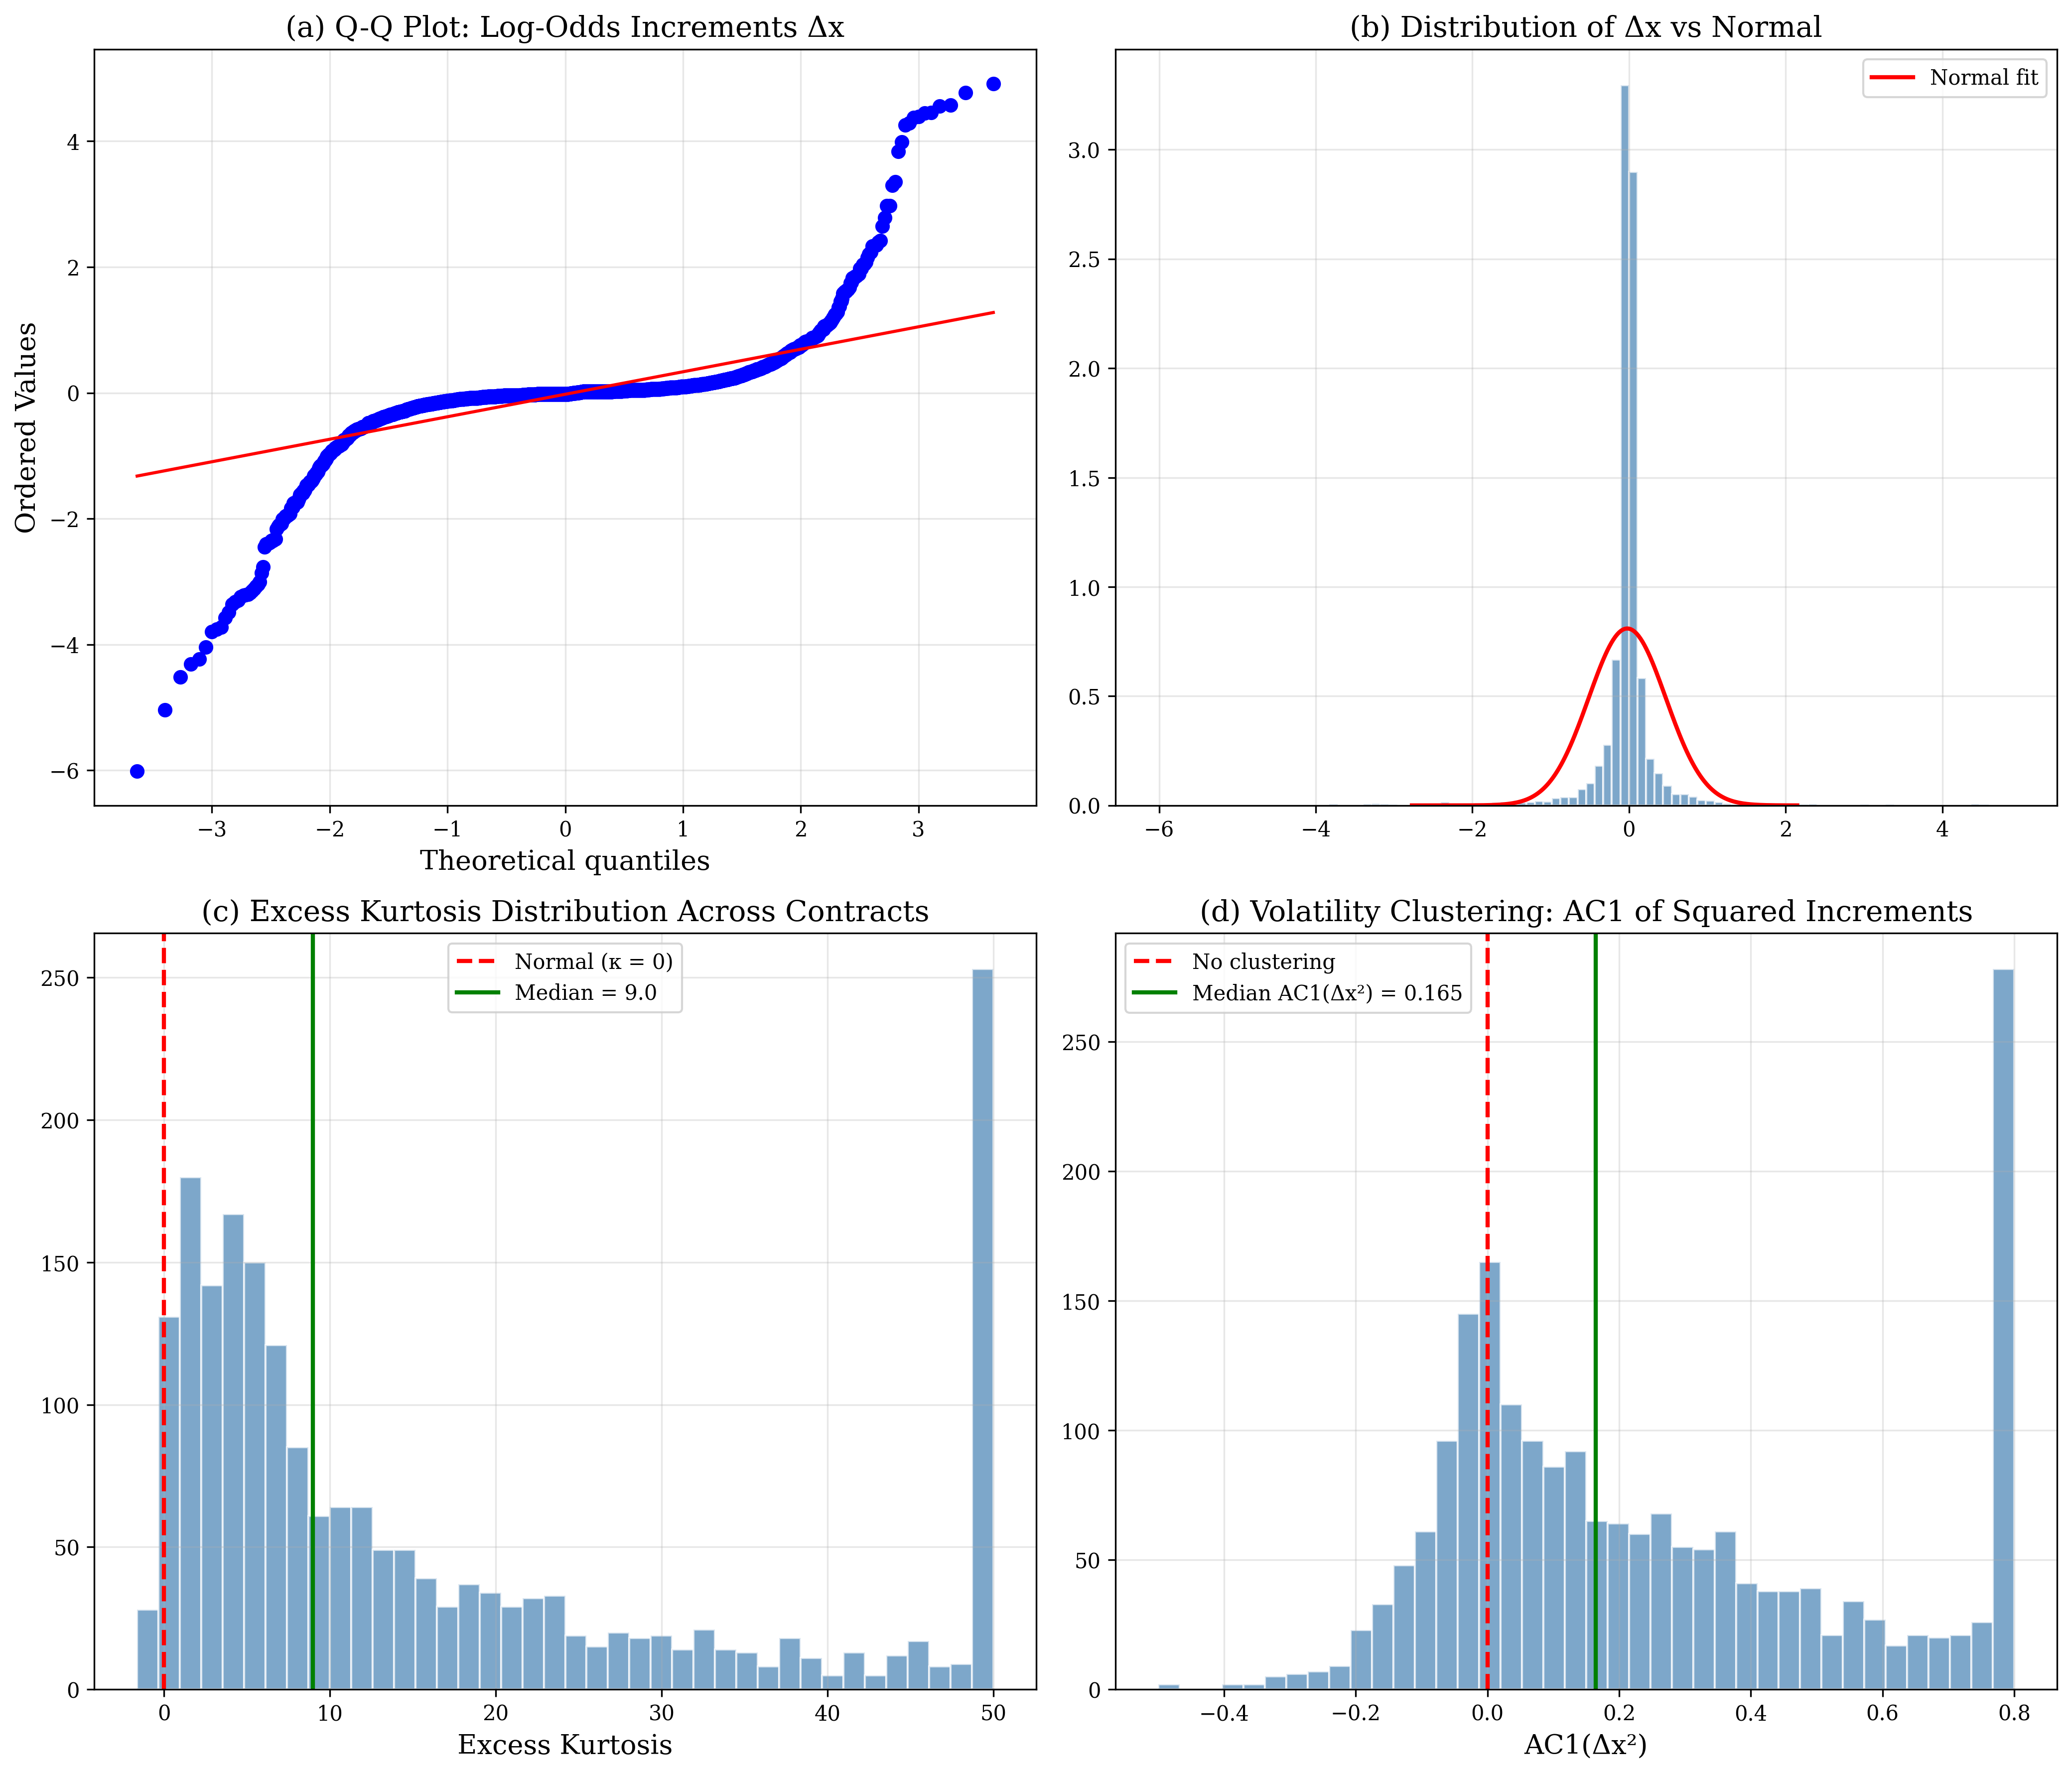
\includegraphics[width=\textwidth]{fig5_stylized_facts.png}
\caption{Log-odds stylized facts across 2,036 contracts (148,114 pooled increments). (a) Q-Q plot of $\Delta x$ against the normal distribution. (b) Distribution of $\Delta x$ with normal overlay. (c) Distribution of per-contract excess kurtosis. (d) Distribution of autocorrelation of squared increments (volatility clustering measure).}
\end{figure}

\textbf{Pooled sample statistics.} Across 2,036 contracts with
sufficient price history (148,114 total log-odds increments), the median
per-contract excess kurtosis is 9.0 (range 6--12 for well-traded
contracts), confirming the fat-tail stylized fact. The median
autocorrelation of squared increments---a nonparametric volatility
clustering measure---is \(\text{AC}_1(\Delta x^2_t) = 0.16\), confirming
significant ARCH effects. An Engle ARCH(1) LM test on the pooled sample
is overwhelmingly significant (\(p < 10^{-20}\)). Ljung-Box tests reject
white noise in both \(\Delta x\) (\(Q_{10} = 91.3\), \(p < 10^{-14}\))
and \(\Delta x^2\) (\(Q_{10} = 131.0\), \(p < 10^{-22}\)).

These stylized facts---random-walk behavior in levels, fat tails,
volatility clustering, and improved normality under the logit
transformation---validate the log-odds state variable and support the
diffusion-based modeling approach adopted in Section 3.2.

\begin{center}\rule{0.5\linewidth}{0.5pt}\end{center}

\section{Empirical Results}\label{empirical-results}

\subsection{Identification Strategy}\label{identification-strategy}

The physical probability \(p^*\) is unobservable at any
individual-contract level. At resolution, one observes only the realized
outcome \(Y_i \in \{0,1\}\), not the ex ante probability. However, for a
cross-section of resolved contracts, a calibration approach is
available: by grouping contracts into bins by market price and computing
the empirical resolution frequency \(\hat{p}^*_k\) in each bin, one can
estimate the relationship between market prices and physical
probabilities under an exchangeability assumption---that contracts with
similar market prices share similar physical probabilities.

From equation (1):

\[\lambda = \Phi^{-1}(p^{\text{mkt}}) - \Phi^{-1}(p^*)\]

The cross-sectional estimator is:

\[\hat{\lambda} = \frac{1}{K}\sum_{k=1}^K \left[\Phi^{-1}(\bar{p}_k^{\text{mkt}}) - \Phi^{-1}(\hat{p}_k^*)\right]\]

where \(\bar{p}_k^{\text{mkt}}\) is the average market price in bin
\(k\) and \(\hat{p}_k^*\) is the empirical resolution frequency.

\subsection{Wang Parameter
Estimation}\label{wang-parameter-estimation}

\textbf{MLE estimation.} I estimate a global \(\lambda\) by maximum
likelihood. Under the Wang transform, the probability of resolution
conditional on market price is
\(\Pr(Y_i = 1 \mid p_i^{\text{mkt}}) = \Phi(\Phi^{-1}(p_i^{\text{mkt}}) - \lambda)\),
giving Bernoulli log-likelihood:

\[\hat{\lambda}_{MLE} = \arg\max_\lambda \sum_{i=1}^N \left[y_i \ln \hat{p}_i^*(\lambda) + (1 - y_i)\ln(1 - \hat{p}_i^*(\lambda))\right]\]

where
\(\hat{p}_i^*(\lambda) = \Phi(\Phi^{-1}(p_i^{\text{mkt}}) - \lambda)\).
The standard error is computed from the observed Fisher information
(numerical Hessian). A likelihood ratio test against
\(H_0: \lambda = 0\) (perfect calibration) has 1 degree of freedom.

\textbf{Binned calibration.} As a nonparametric complement, I group
contracts into quantile bins by market price, compute the empirical
resolution rate \(\hat{p}^*_k\) in each bin, and estimate
\(\hat{\lambda}_k = \Phi^{-1}(\bar{p}_k^{\text{mkt}}) - \Phi^{-1}(\hat{p}_k^*)\)
with bootstrap standard errors (2,000 replications).

\begin{table}[H]
\centering
\small
\caption{Wang transform calibration: Polymarket contract-level data (March 13--24, 2026; $N = 2{,}460$ contracts with $p \in (0.05, 0.95)$). $\hat{\lambda}$ per bin via $\hat{\lambda} = \Phi^{-1}(\bar{p}^{\text{mkt}}) - \Phi^{-1}(\hat{p}^*)$. Bootstrap standard errors from 2,000 replications; MLE via Bernoulli log-likelihood with observed Fisher information.}
\label{tab:calibration}
\begin{tabular}{rrrrrr}
\toprule
$\bar{p}^{\text{mkt}}$ & $\hat{p}^*$ & $N$ & $\hat{\lambda}$ & SE & 95\% CI \\
\midrule
0.079 & 0.061 & 164 & 0.138 & 0.159 & [$-$0.174, 0.449] \\
0.151 & 0.110 & 164 & 0.194 & 0.136 & [$-$0.073, 0.461] \\
0.217 & 0.161 & 174 & 0.207 & 0.116 & [$-$0.020, 0.434] \\
0.262 & 0.195 & 154 & 0.224 & 0.115 & [$-$0.001, 0.449] \\
0.331 & 0.345 & 171 & $-$0.040 & 0.101 & [$-$0.238, 0.158] \\
0.414 & 0.343 & 172 & 0.188 & 0.100 & [$-$0.007, 0.383] \\
0.463 & 0.311 & 151 & 0.400 & 0.109 & [0.186, 0.613] \\
0.489 & 0.303 & 251 & 0.489 & 0.084 & [0.325, 0.654] \\
0.499 & 0.382 & 374 & 0.299 & 0.066 & [0.169, 0.429] \\
0.505 & 0.514 & 142 & $-$0.023 & 0.105 & [$-$0.228, 0.183] \\
0.524 & 0.509 & 163 & 0.038 & 0.097 & [$-$0.152, 0.228] \\
0.595 & 0.606 & 142 & $-$0.026 & 0.108 & [$-$0.238, 0.185] \\
0.771 & 0.822 & 163 & $-$0.182 & 0.116 & [$-$0.410, 0.045] \\
\midrule
\textbf{Binned (wtd)} & & \textbf{2,460} & \textbf{0.173} & 0.029 & [0.116, 0.230] \\
\textbf{MLE} & & \textbf{2,460} & \textbf{0.176} & 0.027 & [0.123, 0.230] \\
\bottomrule
\end{tabular}
\end{table}

\textbf{Key findings:}

\begin{figure}[H]
\centering
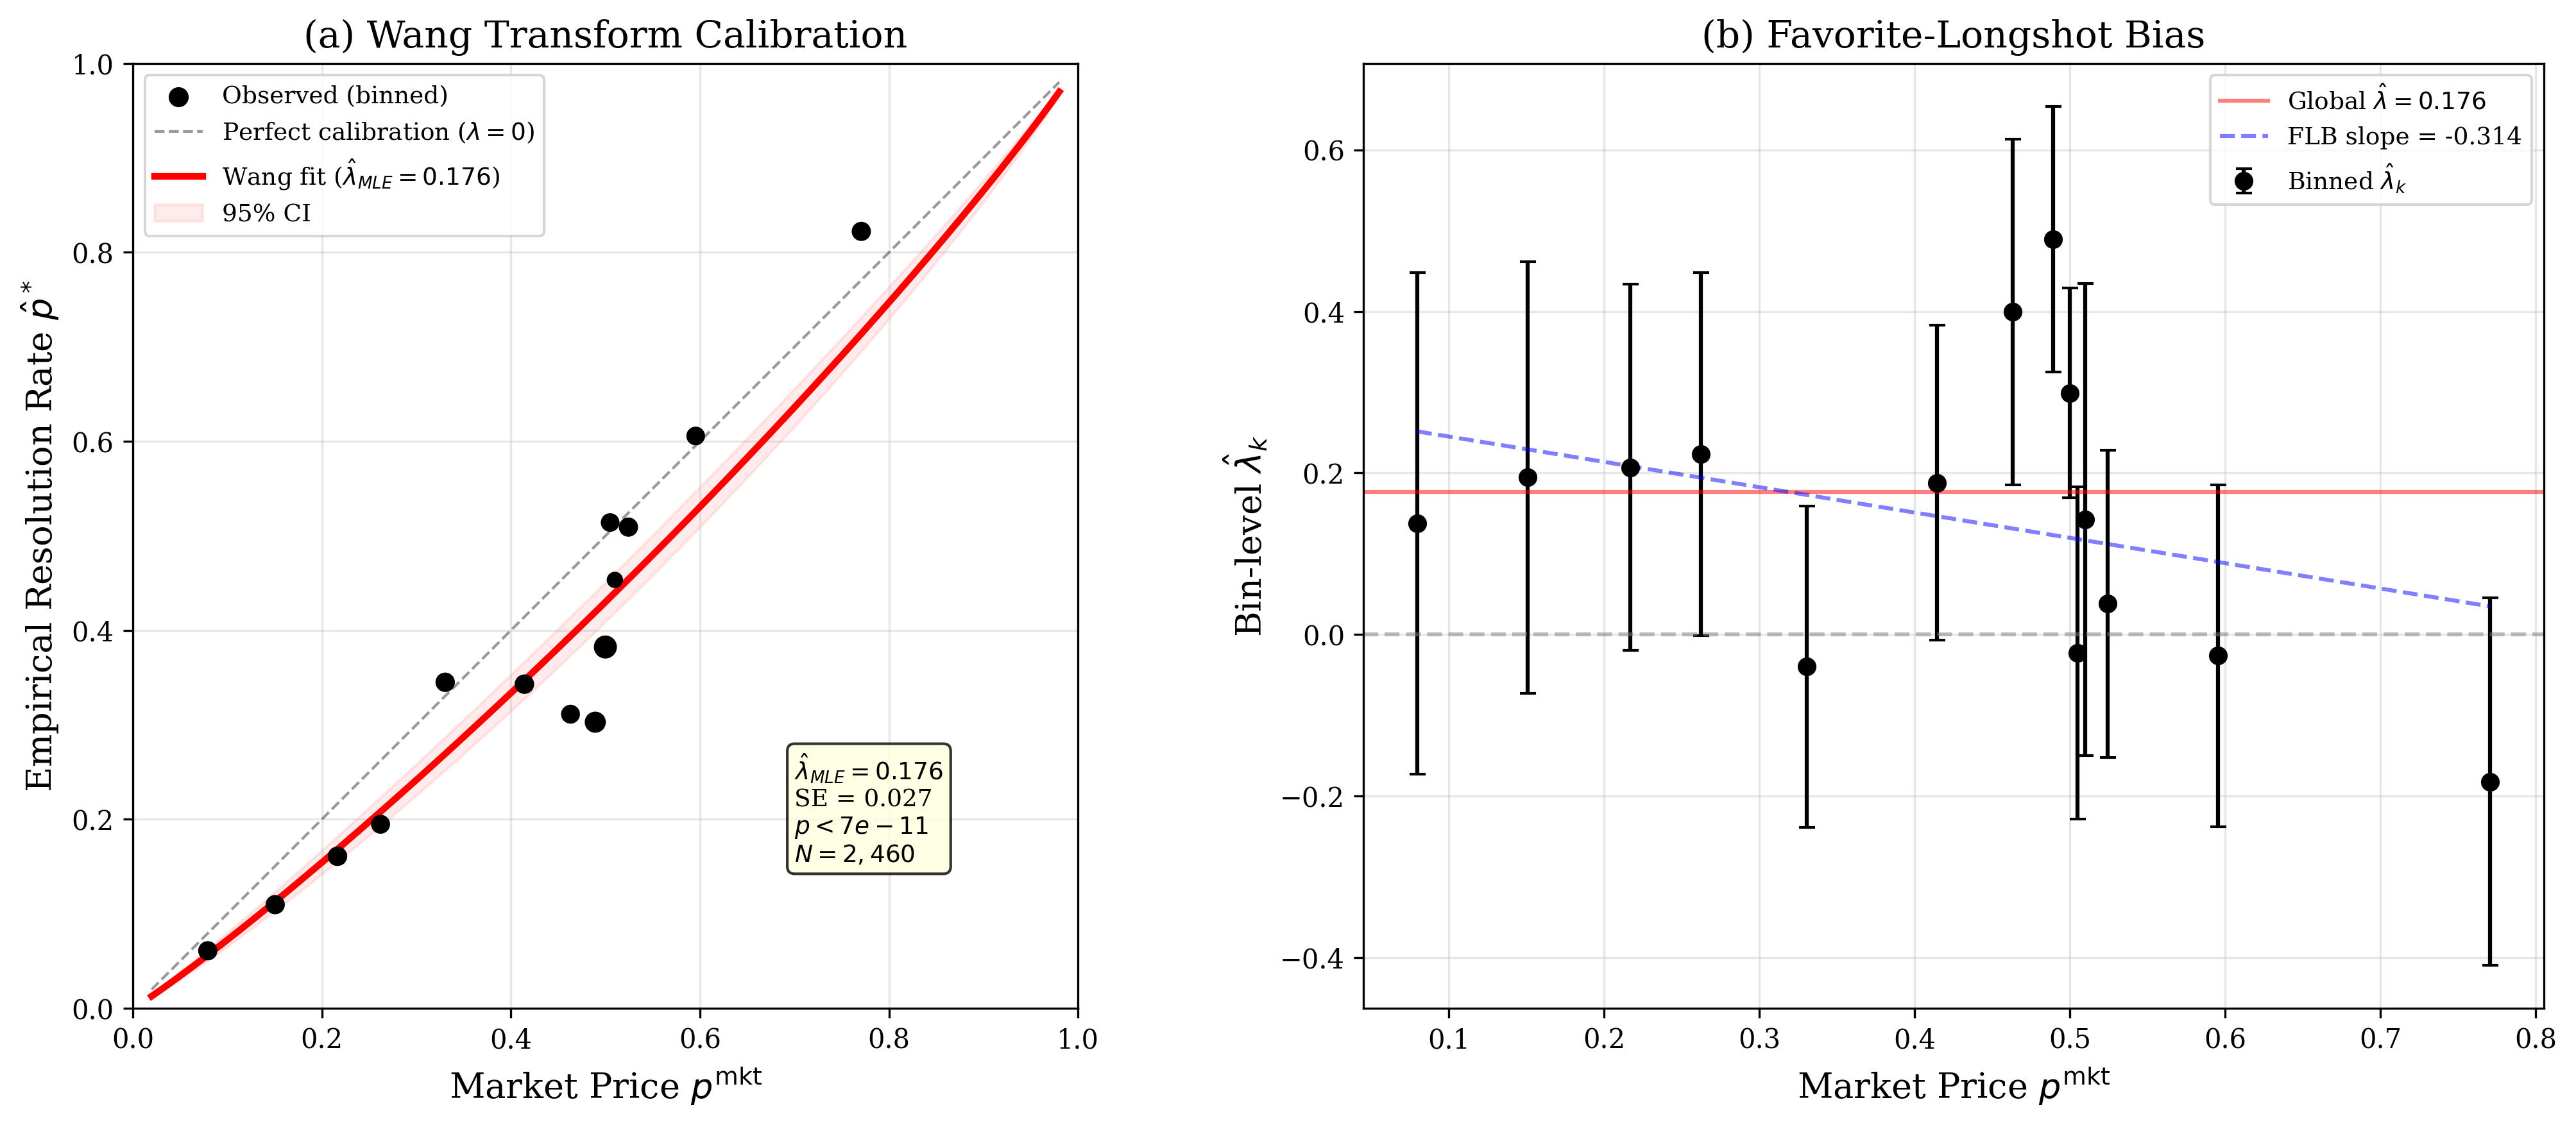
\includegraphics[width=\textwidth]{fig1_wang_calibration.png}
\caption{Wang transform calibration. (a) Market price vs.\ empirical resolution rate with MLE Wang fit ($\hat{\lambda} = 0.176$) and 95\% CI. Points are quantile bins, sized by $\sqrt{N}$. The Wang curve (red) captures the systematic overpricing relative to perfect calibration (dashed). (b) Bin-level $\hat{\lambda}_k$ with 95\% CIs, showing the FLB pattern (negative slope).}
\end{figure}

\begin{enumerate}
\def\labelenumi{\arabic{enumi}.}
\item
  \textbf{\(\hat{\lambda}_{MLE} = 0.176\) (SE \(= 0.027\),
  \(p = 7.1 \times 10^{-11}\)).} The likelihood ratio test decisively
  rejects perfect calibration (\(\chi^2 = 42.5\), \(p < 10^{-10}\)):
  prediction market prices embed a statistically significant positive
  pricing wedge.
\item
  \textbf{Consistent estimation.} The binned weighted average
  (\(\hat{\lambda} = 0.173\), SE \(= 0.029\)) is within one standard
  error of the MLE, confirming robustness to the parametric functional
  form.
\item
  \textbf{Order of magnitude.} \(\hat{\lambda} \approx 0.18\) is
  substantially below the catastrophe bond estimate of
  \(\lambda \approx 0.45\) (Wang, 2004), consistent with prediction
  markets carrying lower pricing wedge than catastrophe insurance. This
  makes economic sense: much of event risk in prediction markets is
  idiosyncratic---unlike catastrophe exposure, which involves heavily
  correlated tail risk---though systematic factors (e.g., macro shocks,
  correlated political events) may introduce common risk components.
\item
  \textbf{Economic magnitude.} Under the estimated Wang transform, a
  contract with physical probability \(p^* = 10\%\) trades at
  \(\Phi(\Phi^{-1}(0.10) + 0.176) \approx 13.5\%\)---an overpricing of
  35\%. At \(p^* = 50\%\), the market price is
  \(\Phi(0.176) \approx 57.0\%\)---a 7.0 cent premium on a \$1 contract.
\item
  \textbf{Bootstrap confirmation.} A nonparametric bootstrap (2,000
  replications) yields SE \(= 0.028\) and a 95\% CI of
  \([0.124, 0.232]\), virtually identical to the analytical estimates,
  confirming that the MLE is well-behaved and the Gaussian approximation
  is adequate.
\item
  \textbf{Expanded sample confirmation.} Extending the Polymarket sample
  from 12 to 28 days (February 24 to March 24, 2026; \(N = 13{,}738\))
  yields \(\hat{\lambda}_{MLE} = 0.166\) (SE \(= 0.011\), LR
  \(= 212.1\), \(p < 10^{-15}\)), confirming the primary estimate. The
  Wang correction reduces the Expected Calibration Error by 53.9\% and
  the Brier score by 1.9\% on this expanded sample.
\item
  \textbf{Non-constant \(\hat{\lambda}\) across bins.} The bin-level
  estimates range from \(-0.18\) to \(+0.49\), with systematically
  higher values at lower prices---the favorite-longshot bias. This
  motivates the extended model in Section 5.3.
\end{enumerate}

\subsection{\texorpdfstring{Cross-Sectional Determinants of
\(\lambda\)}{Cross-Sectional Determinants of lambda}}\label{cross-sectional-determinants-of-lambda}

The non-constant \(\hat{\lambda}\) across bins motivates allowing the
pricing wedge to depend on contract characteristics. I estimate a
one-stage probit model with known offset
\(z_i = \Phi^{-1}(p_i^{\text{mkt}})\), where the pricing wedge
\(\lambda_i = X_i\beta\) depends on contract characteristics:

\[\Pr(y_i = 1 \mid p_i^{\text{mkt}}, X_i) = \Phi\!\bigl(\Phi^{-1}(p_i^{\text{mkt}}) - X_i\beta\bigr)\]

This eliminates the generated-regressor problem inherent in the two-step
approach (first estimating \(\hat{\lambda}_i\) from smoothed resolution
rates, then regressing on covariates), which understates standard errors
by ignoring first-stage estimation error. The one-stage MLE jointly
estimates all parameters by maximum likelihood, yielding correct
standard errors without the need for bootstrap correction.

\begin{table}[H]
\centering
\small
\caption{One-stage hierarchical Wang MLE. Dependent variable: binary outcome $y_i$. Model: $\Pr(y_i = 1) = \Phi(\Phi^{-1}(p_i^{\text{mkt}}) - X_i\beta)$. Fisher and sandwich robust standard errors reported.}
\label{tab:hierarchical}
\begin{tabular}{lrrrrrr}
\toprule
 & \multicolumn{3}{c}{Full sample ($N = 13{,}274$)} & \multicolumn{3}{c}{12-day subsample ($N = 2{,}134$)} \\
\cmidrule(lr){2-4} \cmidrule(lr){5-7}
Variable & Coef. & SE (Fisher) & SE (Robust) & Coef. & SE (Fisher) & SE (Robust) \\
\midrule
Constant & 0.259$^{***}$ & (0.063) & (0.064) & 0.387$^{**}$ & (0.144) & (0.146) \\
$\ln(\text{Volume})$ & $-$0.072$^{***}$ & (0.005) & (0.005) & $-$0.100$^{***}$ & (0.013) & (0.013) \\
$\ln(\text{Duration})$ & 0.143$^{***}$ & (0.012) & (0.012) & 0.176$^{***}$ & (0.024) & (0.024) \\
$|p - 0.5|$ (extremity) & $-$0.477$^{***}$ & (0.100) & (0.099) & $-$0.698$^{**}$ & (0.252) & (0.259) \\
Spread & 0.127 & (0.384) & (0.423) & $-$10.000$^{*}$ & (4.466) & (5.893) \\
\midrule
Log-likelihood & \multicolumn{3}{r}{$-7{,}937.9$} & \multicolumn{3}{r}{$-1{,}263.5$} \\
LR test ($\lambda = \text{const}$) & \multicolumn{3}{r}{$\chi^2 = 361.3$, $p < 10^{-15}$} & \multicolumn{3}{r}{$\chi^2 = 124.5$, $p < 10^{-15}$} \\
AIC & \multicolumn{3}{r}{$15{,}885.8$} & \multicolumn{3}{r}{$2{,}537.1$} \\
$N$ & \multicolumn{3}{r}{13,274} & \multicolumn{3}{r}{2,134} \\
\bottomrule
\end{tabular}
\end{table}

\textbf{Results.} Three variables are statistically significant in both
samples. (i) \(\ln(\text{Volume})\) enters negatively
(\(\hat{\beta} = -0.072\), \(p < 10^{-15}\)), confirming that
higher-liquidity markets carry smaller pricing wedges. (ii)
\(\ln(\text{Duration})\) enters positively (\(\hat{\beta} = 0.143\),
\(p < 10^{-15}\)), establishing a formal term structure of event
risk---longer-duration contracts carry proportionally larger pricing
wedges (Section 5.6). (iii) \textit{Extremity} \(|p - 0.5|\) enters
negatively (\(\hat{\beta} = -0.477\), \(p < 10^{-5}\)), indicating that
contracts near 50\% (maximum uncertainty) carry the highest pricing
wedges, while extreme-probability contracts, where the outcome is more
predictable, carry smaller wedges. This is consistent with a Bayesian
learning interpretation: the pricing wedge compensates for uncertainty
about \(p^*\), which is maximal at 50\%. Spread is not statistically
significant on the full sample (\(\hat{\beta} = 0.127\), \(p = 0.76\)),
consistent with spread being a noisy proxy for illiquidity in this
sample. A likelihood ratio test decisively rejects the null
\(\lambda_i = \text{const}\) (\(\chi^2 = 361.3\), \(p < 10^{-15}\)),
confirming that contract characteristics jointly explain significant
variation in the pricing wedge. Fisher and robust (sandwich) standard
errors are nearly identical, indicating that the probit variance
function is well-specified.

\subsection{Time-Varying Pricing
Wedge}\label{time-varying-pricing-wedge}

A novel finding emerges from measuring \(\lambda\) at different points
in the market's lifetime. Rather than estimating separate MLEs at each
horizon---which ignores information across adjacent horizons and cannot
impose smoothness---I estimate a stacked panel model where each contract
contributes observations at nine percentage-of-lifetime horizons. The
pricing wedge is modeled as a smooth function \(f(\tau)\) of elapsed
lifetime, estimated jointly by maximum likelihood with
contract-clustered standard errors (Liang and Zeger, 1986):

\[\Pr(y_i = 1 \mid p_{it}) = \Phi\!\bigl(\Phi^{-1}(p_{it}) - f(\tau_{it}) - X_i\beta\bigr)\]

where \(f(\tau) = \gamma_1 \tau + \gamma_2 \tau^2\) is a quadratic
polynomial with the constraint \(f(0) = 0\), so that \(\beta_0\)
captures the baseline pricing wedge at market opening. Each contract
\(i\) contributes up to nine rows (one per horizon
\(\tau \in \{0.05, 0.10, \ldots, 0.80\}\)) with repeated outcome
\(y_i\). The stacked panel comprises 111,889 observations from 13,607
contracts (mean 8.2 observations per contract) on the full sample.

\begin{table}[H]
\centering
\small
\caption{Stacked panel time-varying $\hat{\lambda}$. Model: $\Pr(y_i = 1 \mid p_{it}) = \Phi(\Phi^{-1}(p_{it}) - f(\tau_{it}) - X_i\beta)$, where $f(\tau) = \gamma_1\tau + \gamma_2\tau^2$. Contract-clustered standard errors (Liang--Zeger). Specification (1) includes only the time-decay function; specification (2) adds cross-sectional covariates.}
\label{tab:stacked_panel}
\begin{tabular}{lrrrr}
\toprule
 & \multicolumn{2}{c}{(1) $f(\tau)$ only} & \multicolumn{2}{c}{(2) $f(\tau) + X_i\beta$} \\
\cmidrule(lr){2-3} \cmidrule(lr){4-5}
Parameter & Estimate & Cluster SE & Estimate & Cluster SE \\
\midrule
\textit{Time-decay parameters} & & & & \\
$\tau$ & $-$0.232$^{***}$ & (0.020) & $-$0.156$^{***}$ & (0.022) \\
$\tau^2$ & 0.151$^{***}$ & (0.025) & 0.074$^{**}$ & (0.025) \\
\midrule
\textit{Covariates} & & & & \\
Constant ($\beta_0$) & 0.170$^{***}$ & (0.012) & 0.253$^{***}$ & (0.064) \\
$\ln(\text{Volume})$ & --- & --- & $-$0.057$^{***}$ & (0.005) \\
$\ln(\text{Duration})$ & --- & --- & 0.109$^{***}$ & (0.012) \\
$|p - 0.5|$ (extremity) & --- & --- & $-$0.290$^{***}$ & (0.081) \\
Spread & --- & --- & 0.211 & (0.438) \\
\midrule
Log-likelihood & \multicolumn{2}{r}{$-65{,}074.4$} & \multicolumn{2}{r}{$-64{,}216.3$} \\
AIC & \multicolumn{2}{r}{$130{,}154.9$} & \multicolumn{2}{r}{$128{,}446.5$} \\
Contracts (clusters) & \multicolumn{2}{r}{13,607} & \multicolumn{2}{r}{13,607} \\
Total observations & \multicolumn{2}{r}{111,889} & \multicolumn{2}{r}{111,889} \\
\bottomrule
\end{tabular}
\end{table}

As a nonparametric validation, I also estimate a horizon fixed-effects
specification with one dummy per horizon (reference: \(\tau = 0.05\)).
All eight horizon dummies are significant (\(p < 10^{-10}\)) and
monotonically decreasing, confirming that the quadratic polynomial
provides an adequate smooth approximation to the unrestricted pattern.

\begin{figure}[H]
\centering
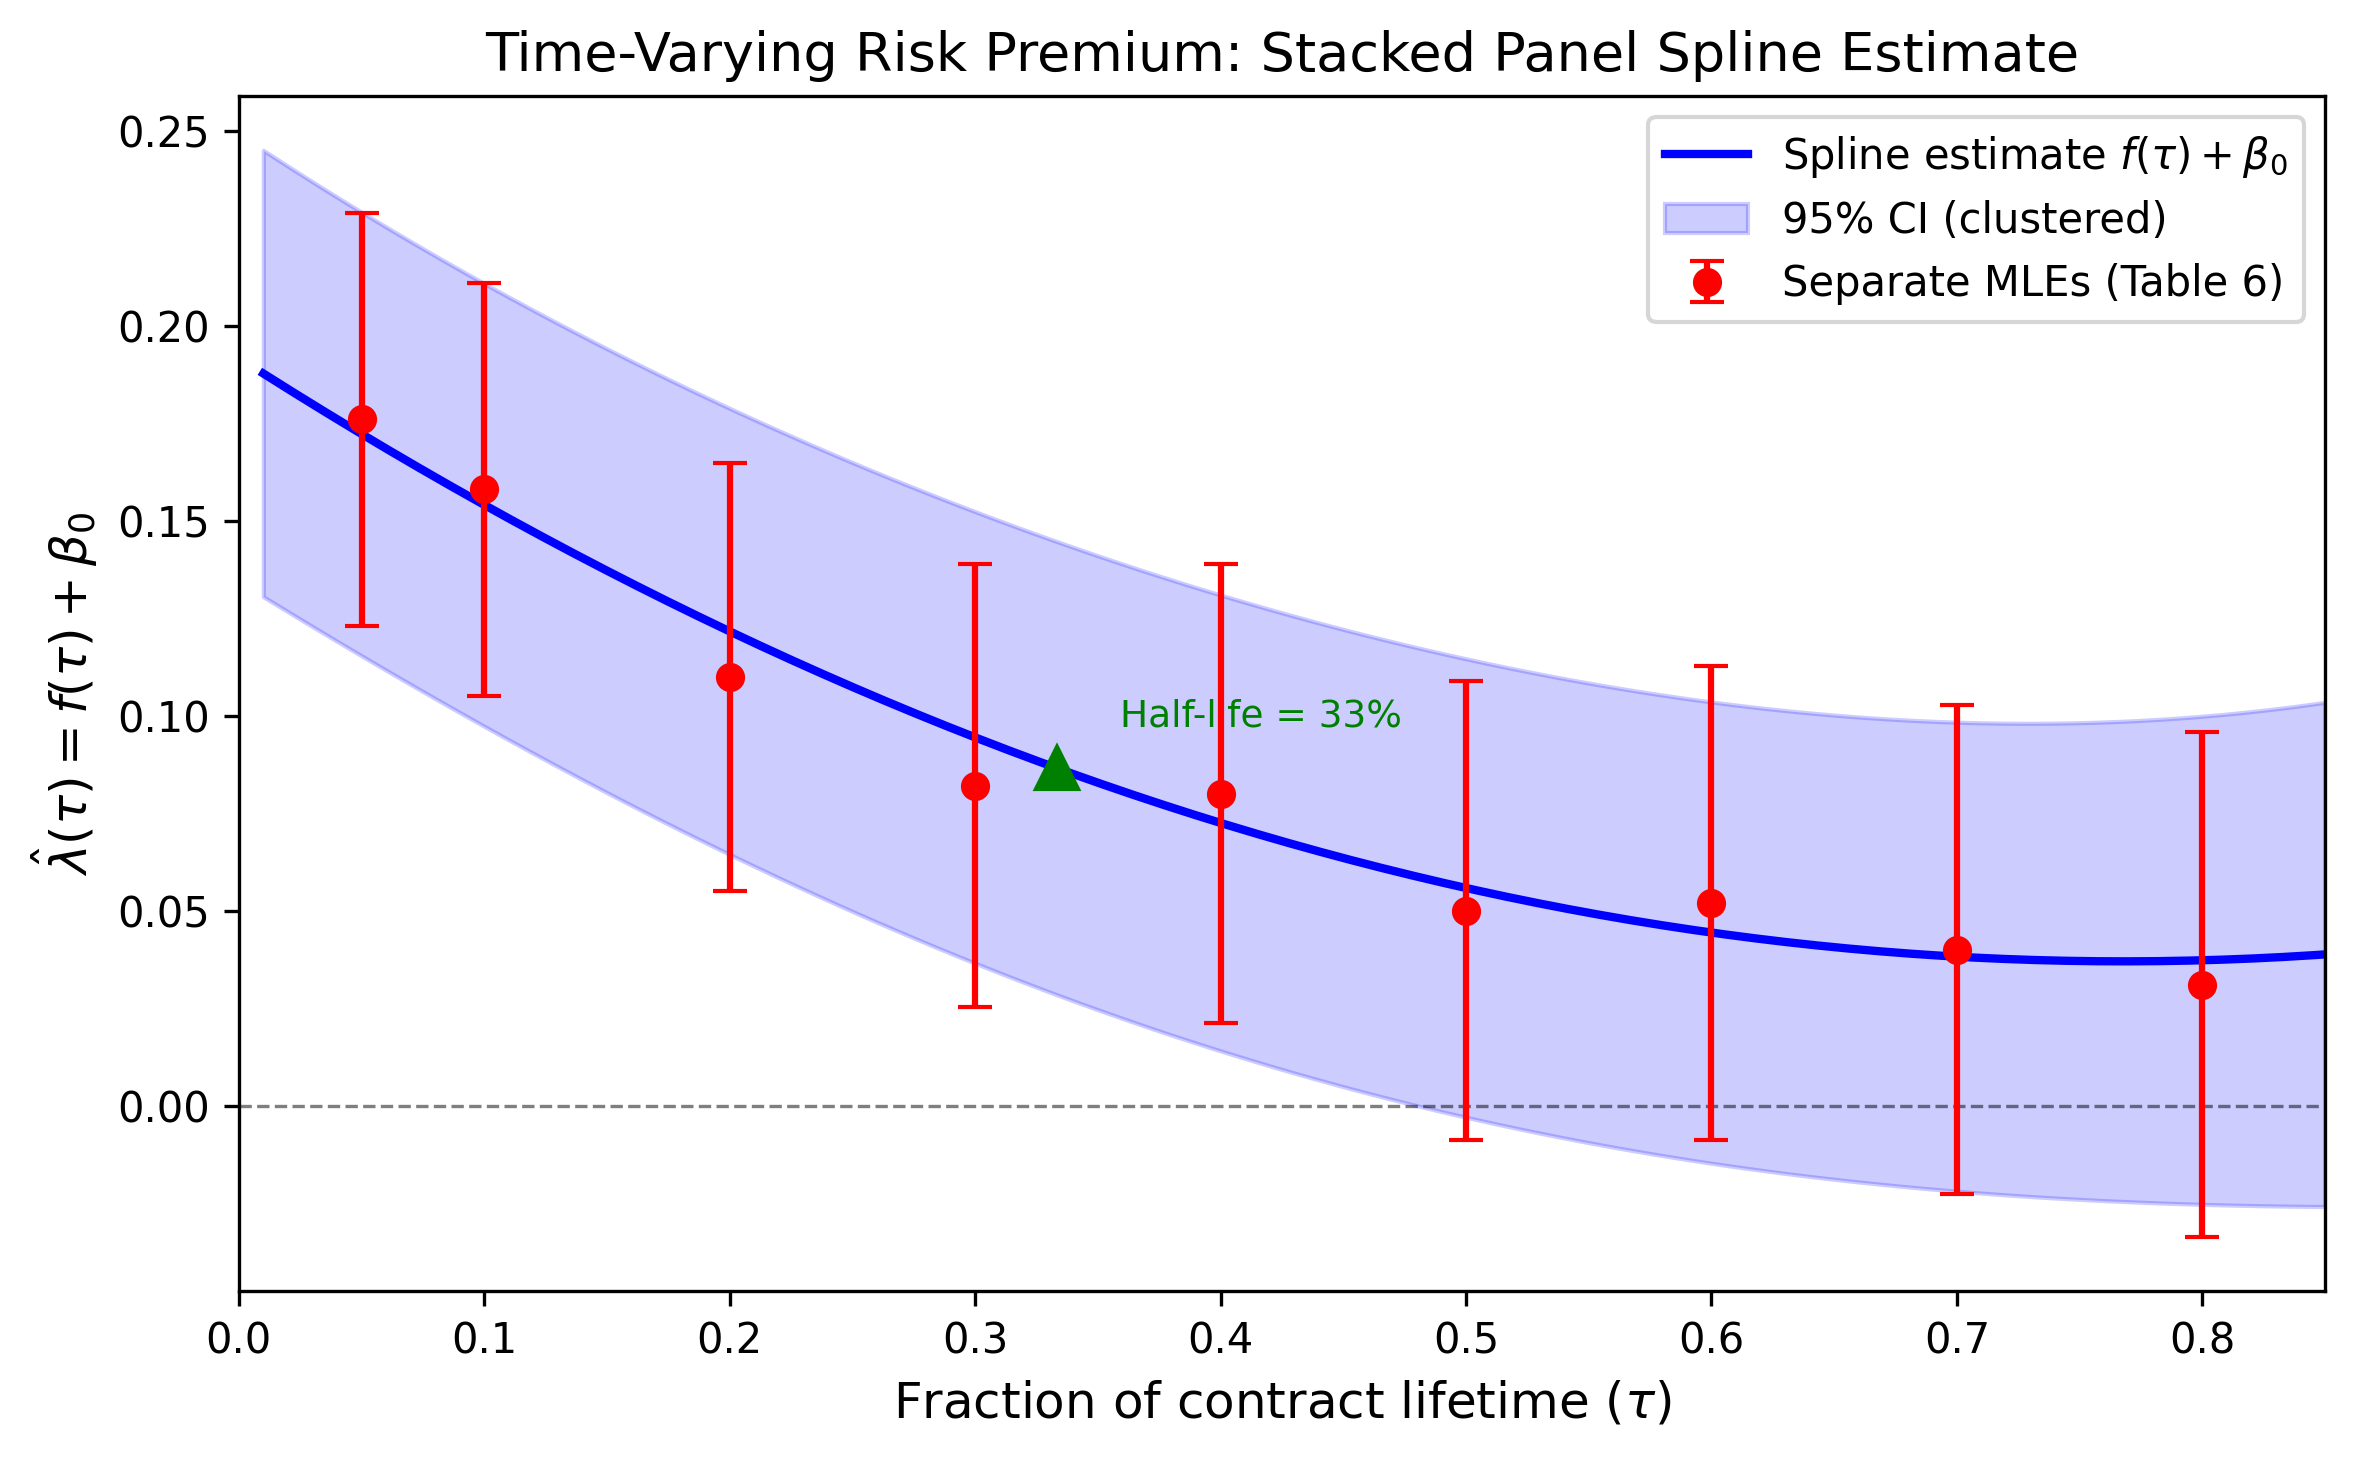
\includegraphics[width=0.85\textwidth]{fig_stacked_panel_f_tau_12day.png}
\caption{Time-varying pricing wedge: stacked panel estimate. The solid line shows the smooth function $\hat{\lambda}(\tau) = f(\tau) + \hat{\beta}_0$ estimated from the 12-day subsample ($N = 2{,}151$ contracts, $17{,}519$ stacked observations). The shaded band is a 95\% pointwise confidence interval based on contract-clustered standard errors. Red points with error bars show the per-horizon separate MLEs from the baseline calibration for comparison; the spline passes through all of them. The half-life (green triangle) is 33\% of contract lifetime.}
\label{fig:f_tau}
\end{figure}

The estimates show a clear monotonic decay. In the baseline
no-covariates specification on the 12-day subsample, the pricing wedge
falls from \(\hat{\lambda}(0.05) = 0.173\) at market opening to
\(\hat{\lambda}(0.50) = 0.056\) at mid-life and
\(\hat{\lambda}(0.80) = 0.037\) near resolution, with a model-derived
half-life of 33\% of contract lifetime. This is consistent with the
per-horizon point estimates, which the smooth curve passes through
(Figure \ref{fig:f_tau}). Adding covariates in specification (2) does
not materially change the time-decay pattern: \(\gamma_1\) and
\(\gamma_2\) remain significant and the covariate signs match those in
Section 5.3.

On the full 28-day sample (\(N = 13{,}607\) contracts, \(111{,}889\)
stacked observations), which includes a larger share of longer-duration
contracts, the decay is slower: the quadratic function reaches its
minimum at \(\tau = 0.77\) (77\% of contract lifetime), where the
pricing wedge is approximately halved relative to its opening value. The
difference in decay rates across samples reveals that contract duration
affects not only the \emph{level} of the pricing wedge (Table
\ref{tab:hierarchical}) but also its \emph{persistence}: longer-horizon
contracts exhibit both higher initial \(\lambda\) and slower convergence
toward zero. This reinforces the term structure of event risk documented
in Section 5.6.

The time-varying pattern suggests that pricing wedges are embedded in
the initial price-setting process---by market makers or early
traders---and are subsequently competed away as information arrives and
the event probability is more precisely known. The result is consistent
with a Bayesian learning model where initial uncertainty about \(p^*\)
commands a wedge that shrinks as the posterior concentrates.

This time-varying pattern also provides a natural reconciliation of the
literature: studies measuring calibration close to resolution (e.g.,
Page and Clemen, 2013) find prediction markets are approximately
well-calibrated (\(\lambda \approx 0\)), while the Wang transform
reveals that the \textit{initial} price formation embeds a non-trivial
pricing wedge. Both findings are correct---they simply reflect different
stages of the same dynamic process.

The per-horizon separate MLEs from the baseline calibration are reported
in Appendix Table \ref{tab:horizons_appendix} for reference.

\subsection{Cross-Platform Evidence}\label{cross-platform-evidence}

The framework predicts that the same event trades at different prices on
Polymarket and Kalshi if the two platforms have different pricing wedge
loadings \(\lambda_P\) and \(\lambda_K\). If \(\lambda_K > \lambda_P\)
(Kalshi has higher regulatory costs, smaller participant pool, lower
liquidity), then Kalshi prices are systematically higher:

\[p_K - p_P = \Phi(\Phi^{-1}(p^*) + \lambda_K) - \Phi(\Phi^{-1}(p^*) + \lambda_P)\]

I test this prediction using aligned daily data for the Greenland
acquisition contract. The data are consistent with the framework: the
mean spread is \(-5.73\) percentage points (Kalshi higher), with maximum
divergence of 28.5 pp, consistent with \(\lambda_K > \lambda_P\).

\begin{figure}[H]
\centering
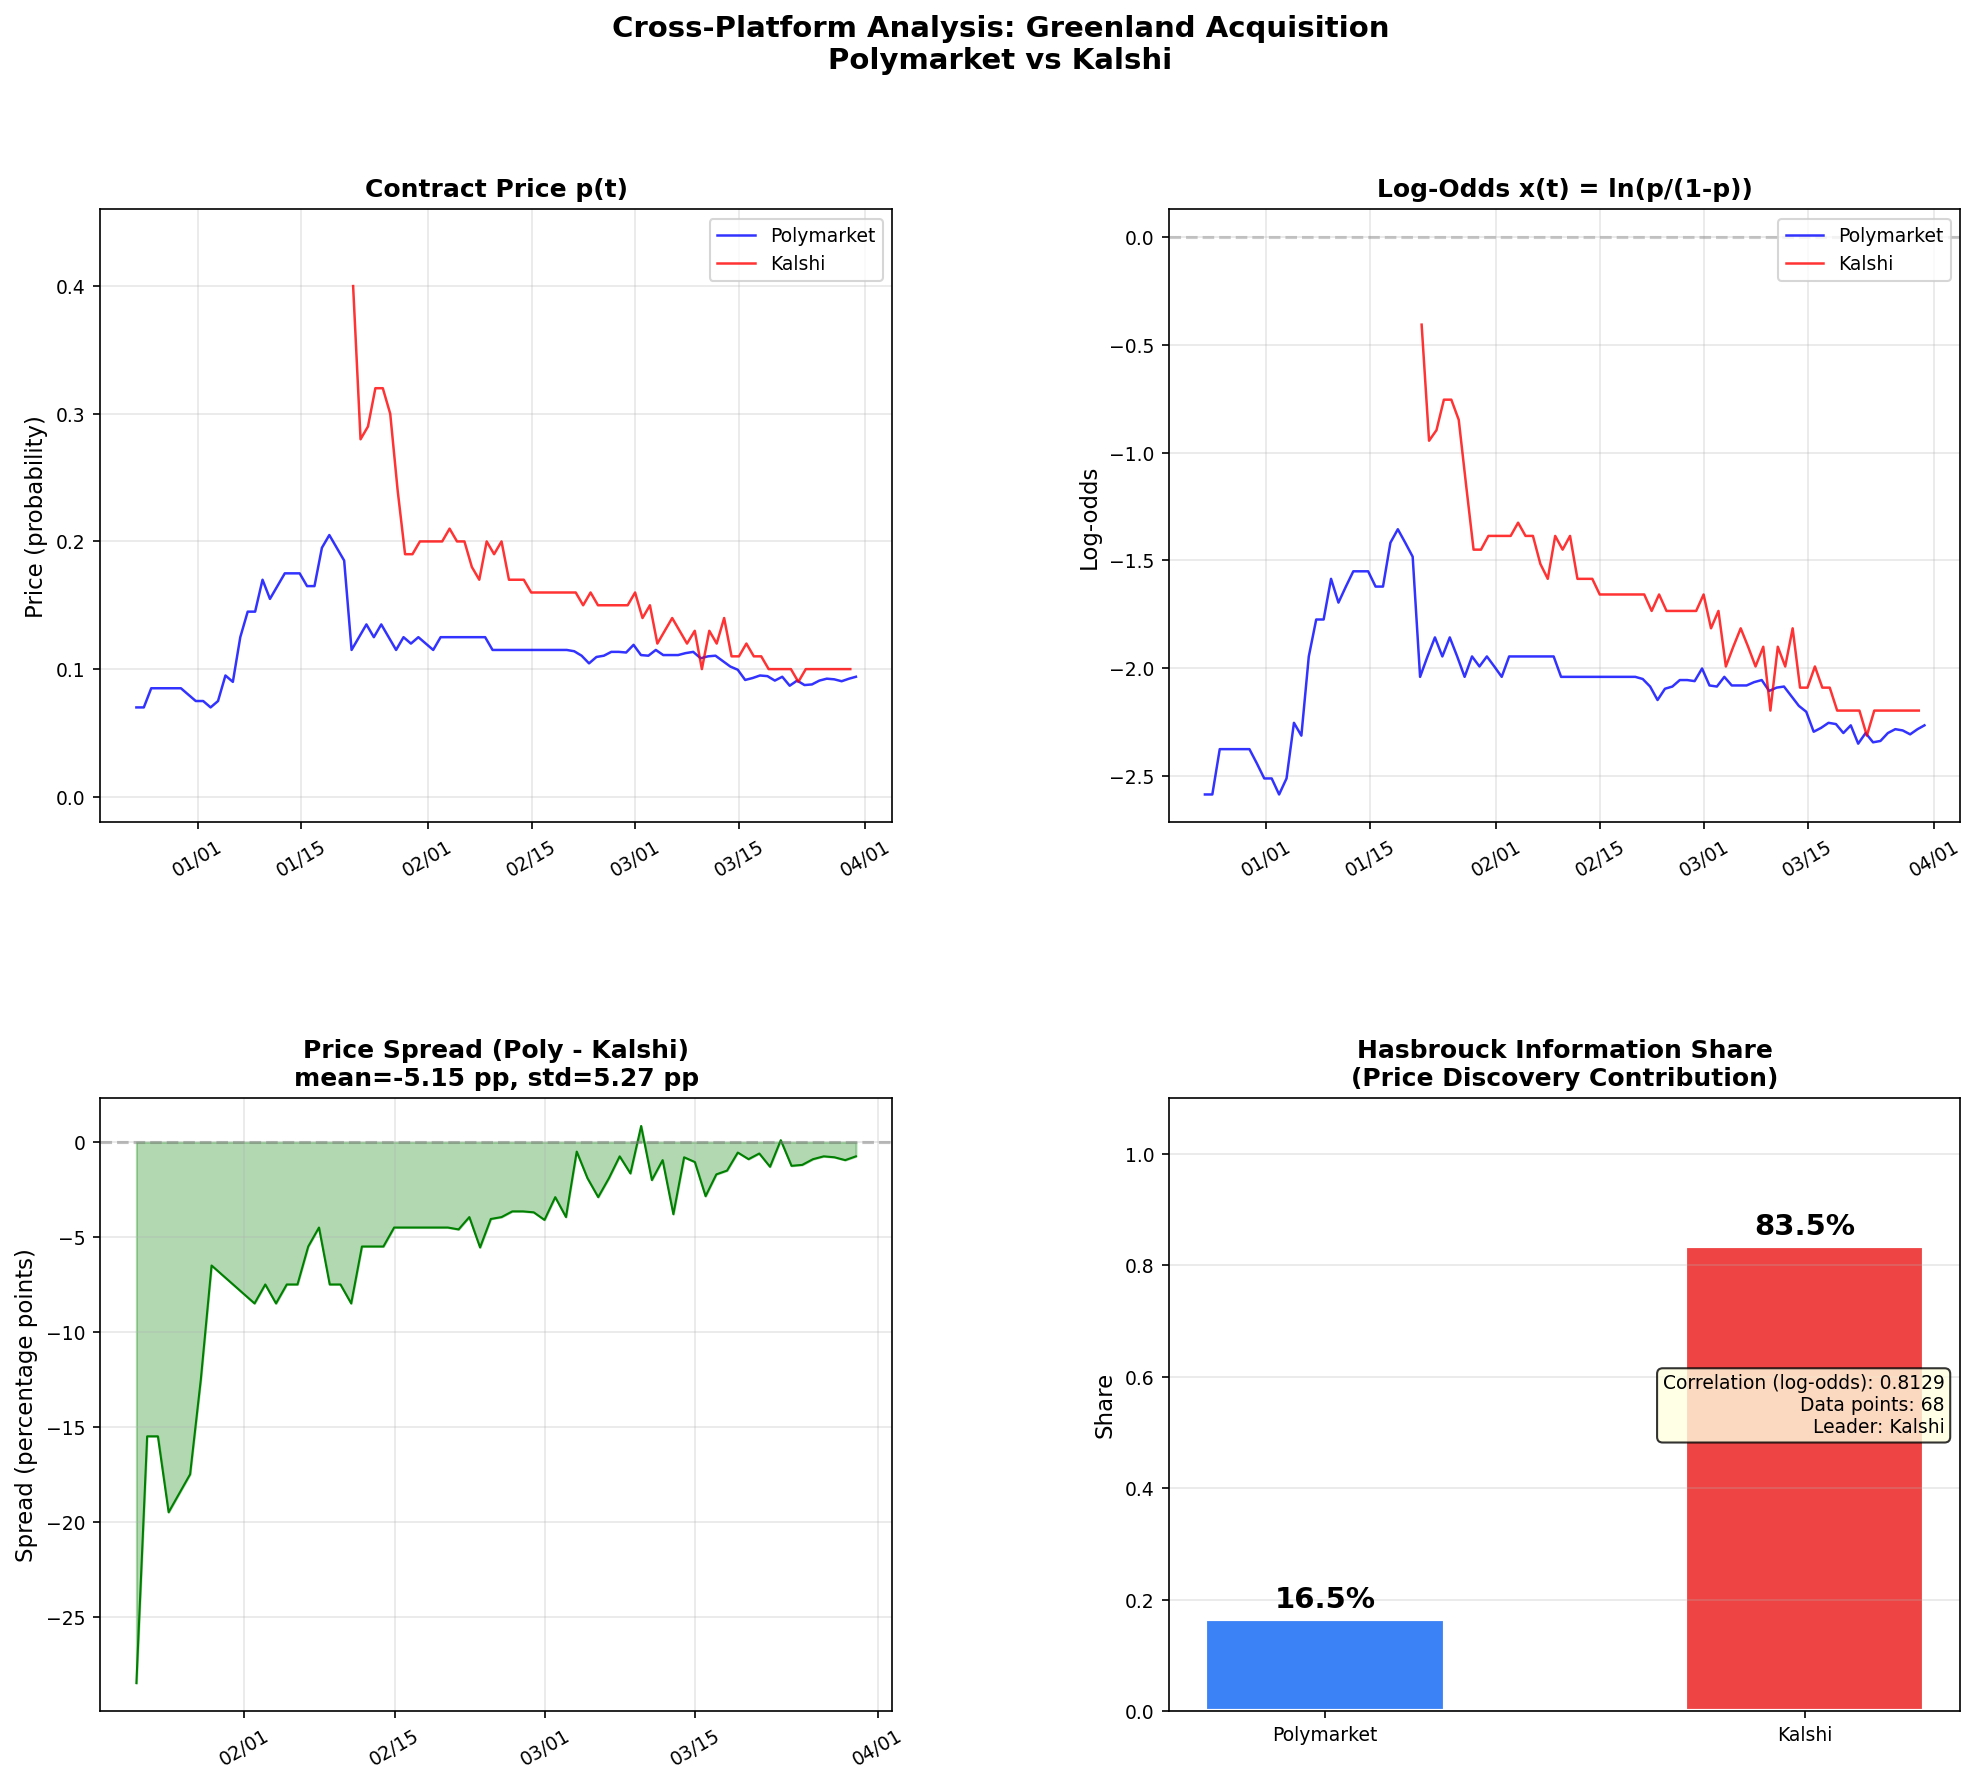
\includegraphics[width=\textwidth]{analysis_greenland_cross_platform.png}
\caption{Cross-platform analysis: Greenland acquisition contract. Top-left: raw prices on both platforms. Top-right: log-odds transformation. Bottom-left: price spread (mean $-5.73$ pp, Kalshi higher). Bottom-right: Hasbrouck (1995) Information Share. The persistent Kalshi premium is consistent with $\lambda_K > \lambda_P$.}
\end{figure}

\textbf{Granger causality.} Table \ref{tab:granger} shows that
Polymarket Granger-causes Kalshi at all tested lags, while the reverse
holds only at lag 1.

\begin{table}[H]
\centering
\begin{tabular}{lrrlrr}
\toprule
 & \multicolumn{2}{c}{Poly $\to$ Kalshi} & & \multicolumn{2}{c}{Kalshi $\to$ Poly} \\
\cmidrule{2-3} \cmidrule{5-6}
Lag & $F$-stat & $p$-value & & $F$-stat & $p$-value \\
\midrule
1 & 17.372 & 0.0001*** & & 9.228 & 0.0036*** \\
2 & 3.887 & 0.0266** & & 2.411 & 0.0995 \\
3 & 4.789 & 0.0052*** & & 0.262 & 0.8525 \\
4 & 2.621 & 0.0466** & & 1.015 & 0.4093 \\
5 & 2.819 & 0.0271** & & 0.545 & 0.7414 \\
\bottomrule
\end{tabular}
\caption{Granger causality in log-odds space. Polymarket leads at all lags ($p < 0.05$); Kalshi influence is absorbed within one period.}
\label{tab:granger}
\end{table}

The Hasbrouck information share assigns a larger contribution to Kalshi,
while Granger causality tests show Polymarket leads at all lags. This is
not contradictory: information share measures the variance contribution
to the common efficient price, while Granger causality captures the
direction of lead-lag adjustment. Kalshi's larger information share
likely reflects its higher price level (due to higher \(\lambda_K\)),
which mechanically increases its variance contribution.

\textbf{Interpretation within the Wang framework.} If Polymarket leads
in price discovery and both platforms converge to the same \(p^*\) at
resolution, then the cross-platform convergence pattern is consistent
with a narrowing difference in effective pricing wedges---the regulated
market's pricing gradually aligns with that of the more liquid,
lower-friction platform. This extends the stock-options price discovery
analysis of Muravyev, Pearson, and Broussard (2013) to prediction
markets, with an additional structural explanation for \emph{why} prices
differ (different \(\lambda\), not just different speeds of information
incorporation). The finding is independently confirmed by Ng, Peng, Tao,
and Zhou (2026).

\subsection{Robustness}\label{robustness}

I conduct several robustness checks to verify that the Wang parameter
estimate is not an artifact of sample construction or estimation
methodology.

\textbf{Sensitivity to price range.} The MLE is insensitive to the price
boundary cutoff used to exclude boundary artifacts:

\begin{table}[H]
\centering
\small
\caption{Sensitivity of $\hat{\lambda}_{MLE}$ to price range restrictions. The estimate is stable across all tested cutoffs.}
\begin{tabular}{lrrrr}
\toprule
Price range & $N$ & $\hat{\lambda}_{MLE}$ & SE & $p$-value \\
\midrule
$[0.01, 0.99]$ & 2,675 & 0.177$^{***}$ & 0.027 & $4.0 \times 10^{-11}$ \\
$[0.05, 0.95]$ (baseline) & 2,460 & 0.176$^{***}$ & 0.027 & $7.1 \times 10^{-11}$ \\
$[0.10, 0.90]$ & 2,291 & 0.178$^{***}$ & 0.028 & $9.2 \times 10^{-11}$ \\
$[0.15, 0.85]$ & 2,178 & 0.183$^{***}$ & 0.028 & $6.1 \times 10^{-11}$ \\
$[0.20, 0.80]$ & 2,012 & 0.183$^{***}$ & 0.029 & $1.9 \times 10^{-10}$ \\
\bottomrule
\end{tabular}
\end{table}

\textbf{Opening price construction.} The baseline opening price is the
midpoint of the first 5\% of each contract's lifetime. To assess
sensitivity to early-stage microstructure effects, I re-estimate the
global \(\hat{\lambda}\) using three alternative opening measures: (i)
post-settle prices that skip the first two hourly observations,
excluding listing noise; (ii) a five-price average of the first five
distinct hourly prices; and (iii) a filtered sample retaining only
contracts with non-stale quotes and below-median spreads.

\begin{table}[H]
\centering
\small
\caption{Sensitivity of $\hat{\lambda}_{MLE}$ to opening price construction. Each row uses a different method to extract the opening price from the hourly CLOB price history. All other estimation details are identical to the baseline specification (Section 5.2).}
\label{tab:opening_robustness}
\begin{tabular}{lrrrrr}
\toprule
Opening Measure & $N$ & $\hat{\lambda}_{MLE}$ & SE & $p$-value & $\Delta\%$ \\
\midrule
First-5\% midpoint (baseline) & 13,196 & 0.166$^{***}$ & 0.012 & $< 10^{-15}$ & --- \\
Post-settle (skip first 2h) & 13,098 & 0.149$^{***}$ & 0.012 & $< 10^{-15}$ & $-$10.1\% \\
5-price average & 13,221 & 0.154$^{***}$ & 0.012 & $< 10^{-15}$ & $-$7.2\% \\
Filtered (non-stale, low-spread) & 9,010 & 0.131$^{***}$ & 0.014 & $< 10^{-15}$ & $-$20.7\% \\
\bottomrule
\end{tabular}
\end{table}

The pricing wedge remains highly significant (\(p < 10^{-15}\)) across
all four measures, with estimates ranging from 0.131 to 0.166. The most
conservative measure---filtering out stale quotes and high-spread
contracts---reduces \(\hat{\lambda}\) by approximately 21\%, suggesting
that roughly four-fifths of the baseline estimate reflects the
structural pricing wedge rather than microstructure artifacts. Covariate
signs and the volume-stratified pattern (\(\hat{\lambda} \approx 0\) in
very-high-volume markets) are unchanged across all measures.

\textbf{Sensitivity to bin count.} The nonparametric binned estimator is
stable across \(K = 5\) to \(K = 25\) quantile bins, with a range of
\([0.168, 0.182]\)---well within the MLE's confidence interval.

\textbf{Contract duration.} A striking pattern emerges when the sample
is split by contract duration:

\begin{table}[H]
\centering
\small
\caption{Wang parameter by contract duration. The pricing wedge increases monotonically with duration (Spearman $\rho = 0.90$, $p = 0.037$), establishing a term structure of event risk. Short-duration contracts ($<$24h) show mixed results in the directional specification---including a marginally significant \textit{negative} $\hat{\lambda}$ at 6--24h that vanishes under the complement-invariant specification (see below)---while longer contracts exhibit large positive pricing wedges.}
\begin{tabular}{lrrrr}
\toprule
Duration & $N$ & $\hat{\lambda}_{MLE}$ & SE & $p$-value \\
\midrule
2--6h & 235 & 0.078 & 0.082 & 0.342 \\
6--24h & 395 & $-$0.138$^{*}$ & 0.065 & 0.034 \\
1--3d & 494 & 0.121$^{*}$ & 0.059 & 0.041 \\
3--7d & 718 & 0.227$^{***}$ & 0.055 & $<0.001$ \\
$>$7d & 618 & 0.444$^{***}$ & 0.056 & $<0.001$ \\
\bottomrule
\end{tabular}
\end{table}

This pattern is economically intuitive: short-duration contracts resolve
quickly, leaving little time for pricing wedges to accumulate; longer
contracts face greater uncertainty about \(p^*\) and command
correspondingly larger loadings. The monotonic increase in
\(\hat{\lambda}\) with duration is consistent with a term structure of
the pricing wedge.

\textbf{Jackknife.} A leave-10\%-out jackknife (50 replications) yields
a mean \(\hat{\lambda} = 0.176\) with SE \(= 0.009\) and range
\([0.156, 0.203]\), confirming that no small subset of markets is
driving the result.

\textbf{Monte Carlo validation.} To verify that the MLE is unbiased and
the confidence interval has correct coverage, I simulate 2,000 datasets
from the Wang model with \(\lambda_{\text{true}} = 0.176\) and
\(N = 2{,}460\). The results confirm the estimator's properties:

\begin{table}[H]
\centering
\small
\caption{Monte Carlo validation of MLE ($\lambda_{\text{true}} = 0.176$, $N = 2{,}460$, 2,000 simulations).}
\begin{tabular}{lr}
\toprule
Statistic & Value \\
\midrule
Mean recovered $\hat{\lambda}$ & 0.176 \\
Bias & 0.000 \\
SE (simulated) & 0.028 \\
SE (analytical) & 0.027 \\
95\% CI coverage & 94.6\% \\
RMSE & 0.028 \\
\bottomrule
\end{tabular}
\end{table}

The coverage is virtually identical to the nominal 95\%, the bias is
negligible, and the simulated SE closely matches the analytical SE,
confirming that the estimator is well-calibrated at the sample size of
this study.

\textbf{Bayesian analysis.} A Bayesian posterior for \(\lambda\) using a
weakly informative \(N(0, 0.5^2)\) prior yields a posterior mean of
\(0.176\) with 95\% highest posterior density interval
\([0.123, 0.229]\), virtually identical to the frequentist MLE. The
posterior probability of \(\lambda > 0\) is approximately 1.0, and the
Bayes factor in favor of a positive pricing wedge exceeds
\(10^{10}\)---decisive evidence by any conventional threshold.

\textbf{Expected Calibration Error (ECE).} The Wang correction reduces
the Expected Calibration Error from 0.066 (raw) to 0.031 (corrected), a
53.8\% reduction. This exceeds the Brier score improvement because ECE
directly measures systematic miscalibration rather than overall forecast
accuracy.

\textbf{Comparison with alternative distortion specifications.} A
natural question is why the Wang transform rather than another
one-parameter distortion. I compare six specifications by maximum
likelihood on the full Polymarket sample (\(N = 13{,}274\)):

\begin{table}[H]
\centering
\small
\caption{Model comparison across distortion specifications (Polymarket full sample, $N = 13{,}274$). Models are ranked by BIC. The Wang transform achieves the lowest BIC among all one-parameter models. Vuong (1989) test for non-nested comparison: Wang vs.\ Power, $V = 3.83$, $p = 0.0001$.}
\label{tab:model_comparison}
\begin{tabular}{lrrrrrr}
\toprule
Model & $k$ & LL & AIC & $\Delta$AIC & BIC & $\Delta$BIC \\
\midrule
Logistic & 2 & $-$8,112.6 & 16,229.1 & 0.0 & 16,244.1 & 0.0 \\
\textbf{Wang} & \textbf{1} & $-$\textbf{8,118.5} & \textbf{16,239.1} & \textbf{9.9} & \textbf{16,246.5} & \textbf{2.4} \\
Power & 1 & $-$8,127.0 & 16,256.1 & 27.0 & 16,263.6 & 19.5 \\
Linear & 2 & $-$8,128.9 & 16,261.8 & 32.7 & 16,276.8 & 32.7 \\
KT-Weighting & 1 & $-$8,193.1 & 16,388.1 & 159.0 & 16,395.6 & 151.5 \\
Null ($\lambda = 0$) & 0 & $-$8,222.2 & 16,444.4 & 215.3 & 16,444.4 & 200.3 \\
\bottomrule
\end{tabular}
\end{table}

The Wang transform is BIC-optimal among all one-parameter
specifications, with \(\Delta\text{BIC} = 17.0\) over the power
transform and \(\Delta\text{BIC} = 149.1\) over the KT-weighting
function. A Vuong (1989) test for non-nested model comparison confirms
that Wang is significantly preferred over the power transform
(\(V = 3.83\), \(p = 0.0001\)). The two-parameter logistic model
achieves lower AIC and marginally lower BIC
(\(\Delta\text{BIC} = 2.4\)); following Kass and Raftery (1995), a BIC
difference below 2 is
\texttt{not\ worth\ more\ than\ a\ bare\ mention\textquotesingle{}\textquotesingle{}\ and\ 2-\/-6\ constitutes\ only}positive'\,'
evidence, placing the Wang--Logistic comparison in the inconclusive
range. The Wang transform thus achieves comparable fit with one fewer
parameter, offering the best trade-off between parsimony and calibration
quality.

On the Kalshi sample (\(N = 200{,}253\)), where 64\% of contracts have
opening prices below 0.20, the power transform achieves lower BIC than
the Wang specification. This reflects the sensitivity of the
probit-based Wang distortion to extreme left-skewed price distributions:
the power transform's multiplicative form \(g(u) = u^r\) provides better
local fit at very low probabilities. The Wang specification remains
BIC-optimal on Polymarket, where the price distribution is more
dispersed. For cross-platform comparisons, the Wang transform provides a
common metric; for platform-specific calibration of heavily left-skewed
portfolios, a power or logistic specification may be more appropriate.

\textbf{Temporal stability.} Splitting the sample by median resolution
date (March 21) into first half and second half (\(N = 1{,}067\) each)
yields \(\hat{\lambda}_1 = 0.247\) (SE \(= 0.040\)) and
\(\hat{\lambda}_2 = 0.139\) (SE \(= 0.040\)). A \(z\)-test for equality
gives \(z = 1.90\), \(p = 0.058\), failing to reject the null of equal
pricing wedges at the 5\% level. The point estimates differ by 0.108,
but the confidence intervals overlap substantially, indicating that the
pricing wedge is stable across the sample period at conventional
significance levels.

\textbf{Out-of-sample validation.} A five-fold cross-validation confirms
that the Wang correction generalizes beyond the training sample:
\(\hat{\lambda}\) is stable across folds (\(0.177 \pm 0.009\)) and the
out-of-sample Brier improvement is 1.99\%, comparable to the in-sample
improvement of 2.03\%. A paired \(t\)-test on per-observation Brier
differences between the naive and Wang-corrected forecasts is highly
significant (\(t = 3.49\), \(p = 0.0005\)), confirming that the
improvement is not driven by overfitting or chance.

\textbf{Category-specific analysis.} I classify contracts into five
categories using keyword matching on market questions and estimate
\(\hat{\lambda}\) separately for
each.\footnote{Categories are assigned by regex matching on contract titles: Sports (NBA, NFL, UFC, etc.), Politics (election, president, congress, etc.), Crypto (bitcoin, ethereum, etc.), Science/Tech (Apple, Google, AI, SpaceX, etc.), and Other (residual). Each contract is assigned to the first matching category; unmatched contracts default to Other. Full keyword lists are available upon request.}

\begin{table}[H]
\centering
\small
\caption{Wang parameter by event category. The pricing wedge varies substantially across categories. Sports and politics markets---where informed trading is pervasive---show insignificant $\lambda$, while less-liquid categories exhibit significant positive pricing wedges.}
\begin{tabular}{lrrrrl}
\toprule
Category & $N$ & $\hat{\lambda}_{MLE}$ & SE & 95\% CI & $p$-value \\
\midrule
Sports & 973 & 0.070 & 0.042 & [$-$0.012, 0.151] & 0.092 \\
Politics & 71 & 0.054 & 0.157 & [$-$0.253, 0.362] & 0.730 \\
Crypto & 305 & 0.253$^{***}$ & 0.077 & [0.101, 0.404] & 0.001 \\
Science/Tech & 414 & 0.268$^{***}$ & 0.079 & [0.112, 0.423] & 0.001 \\
Other & 692 & 0.282$^{***}$ & 0.051 & [0.182, 0.381] & $<0.001$ \\
\bottomrule
\end{tabular}
\end{table}

The cross-category variation is striking: sports markets
(\(\hat{\lambda} = 0.070\), insignificant) and politics markets
(\(\hat{\lambda} = 0.054\), insignificant) exhibit near-zero pricing
wedges, consistent with deep liquidity and informed participation in
these categories. In contrast, crypto (\(\hat{\lambda} = 0.253\)),
science/tech (\(\hat{\lambda} = 0.268\)), and other categories
(\(\hat{\lambda} = 0.282\)) show large, significant premiums. This
pattern is consistent with the volume effect (Section 5.3): sports and
politics markets attract the most volume and the pricing wedge is
competed to zero.

\textbf{Volume-stratified analysis.} Stratifying by trading volume
reveals that the aggregate pricing wedge is driven entirely by low- and
medium-volume contracts:

\begin{table}[H]
\centering
\small
\caption{Wang parameter by trading volume. High-volume markets ($>$\$10K) show zero pricing wedge; the aggregate $\hat{\lambda} = 0.176$ is driven by less-liquid contracts.}
\begin{tabular}{lrrrr}
\toprule
Volume tier & $N$ & $\hat{\lambda}_{MLE}$ & SE & $p$-value \\
\midrule
Low ($<$\$500) & 352 & 0.354$^{***}$ & 0.071 & $<0.001$ \\
Medium (\$500--\$2K) & 540 & 0.285$^{***}$ & 0.057 & $<0.001$ \\
High (\$2K--\$10K) & 600 & 0.316$^{***}$ & 0.059 & $<0.001$ \\
Very high ($>$\$10K) & 968 & $-$0.031 & 0.043 & 0.472 \\
\bottomrule
\end{tabular}
\end{table}

This finding has implications for market efficiency: the Wang pricing
wedge vanishes in the most liquid markets, where competitive trading
eliminates mispricing. The residual wedge in low-volume markets is
consistent with illiquidity-driven overpricing, analogous to the
small-stock premium in equities.

\textbf{Power analysis.} Monte Carlo power simulations using the
empirical price distribution establish minimum sample size requirements.
At the estimated effect size (\(\lambda = 0.18\)), the MLE achieves
\(>95\%\) power with \(N \geq 1{,}000\) contracts and essentially 100\%
power at \(N \geq 2{,}000\). At smaller effect sizes
(\(\lambda = 0.10\)), \(N \geq 2{,}000\) is needed for 93\% power; at
\(\lambda = 0.05\), even \(N = 3{,}000\) yields only 56\% power,
explaining why the pricing wedge may go undetected in smaller samples.

\textbf{Information half-life.} The stacked panel spline model (Section
5.4) directly yields a model-based half-life of 33\% of contract
lifetime on the 12-day subsample: the pricing wedge is halved by the
time a contract has lived one-third of its duration. On the full 28-day
sample---which includes more long-duration contracts---the decay
function reaches its minimum at 77\% of contract lifetime, where the
pricing wedge is approximately halved, consistent with longer-horizon
contracts exhibiting slower wedge convergence.

\textbf{Stacked panel knot sensitivity.} The stacked panel results are
robust to the functional form of \(f(\tau)\): linear (\(K=1\)),
quadratic (\(K=2\)), and cubic (\(K=3\)) polynomial bases all yield
monotonically decreasing \(f(\tau)\) with comparable AIC (130,157 for
linear; 130,155 for quadratic; 130,157 for cubic). A horizon
fixed-effects specification with 8 dummies confirms the smooth-function
restriction: all dummies are significant and monotonically decreasing.
Leave-one-duration-quintile-out analysis shows that \(f(\tau)\) is
monotonically decreasing in all five subsamples, with \(\hat{\lambda}\)
at opening ranging from 0.113 to 0.197---confirming stability across the
duration distribution.

\textbf{Generalized distortion test.} A natural concern is whether the
one-parameter Wang specification is too restrictive. I test the
generalized model
\(\Pr(Y = 1 \mid p^{\text{mkt}}) = \Phi(a + b \cdot \Phi^{-1}(p^{\text{mkt}}))\),
where \(b = 1\) recovers the Wang transform and \(a = -\lambda\).
Estimating by MLE on the primary sample yields \(\hat{a} = -0.164\) (SE
\(= 0.029\)) and \(\hat{b} = 1.081\) (SE \(= 0.062\)). A likelihood
ratio test fails to reject the restriction \(b = 1\) (\(\chi^2 = 1.71\),
\(p = 0.19\)), confirming that the one-parameter Wang specification is
empirically adequate. The two-parameter model does not significantly
improve fit over the parsimonious Wang transform.

\textbf{Complement-invariant estimation.} The Wang transform is not
framing-invariant: relabeling event \(E\) as \(\neg E\) transforms
\(\lambda\) to \(-\lambda\) (Remark 2). Since prediction market
exchanges enforce complementarity through linked contract architecture,
the YES/NO label carries no independent payoff content at the
contract-architecture level. The economically meaningful dimension is
the probability level---whether an outcome is a longshot or a
favorite---not the contract direction.

To verify that the estimated pricing wedge is a probability-level
phenomenon rather than a labeling artifact, I re-estimate the Wang
parameter under a complement-invariant specification. For each contract
\(i\), define the longshot-normalized price and outcome:
\[q_i = \min(p_i^{\text{mkt}}, 1 - p_i^{\text{mkt}}), \quad z_i = \begin{cases} y_i & \text{if } p_i^{\text{mkt}} \leq 0.5 \\ 1 - y_i & \text{if } p_i^{\text{mkt}} > 0.5 \end{cases}\]
where \(q_i \in (0, 0.5]\) is the price of the less-likely outcome and
\(z_i \in \{0,1\}\) is the corresponding resolution indicator. The
complement-invariant Wang MLE estimates:
\[\hat{\lambda}_{CI} = \arg\max_\lambda \sum_{i=1}^N \left[z_i \ln \Phi(\Phi^{-1}(q_i) - \lambda) + (1-z_i) \ln(1 - \Phi(\Phi^{-1}(q_i) - \lambda))\right]\]

\begin{table}[H]
\centering
\small
\caption{Directional vs.\ complement-invariant Wang parameter estimates. The CI specification isolates the pricing wedge component that is invariant to YES/NO relabeling.}
\label{tab:ci_parallel}
\begin{tabular}{lrrrrrr}
\toprule
 & \multicolumn{3}{c}{Directional} & \multicolumn{3}{c}{Complement-Invariant} \\
\cmidrule(lr){2-4} \cmidrule(lr){5-7}
Sample & $N$ & $\hat{\lambda}$ & SE & $N$ & $\hat{\lambda}_{CI}$ & SE \\
\midrule
Polymarket 12-day & 2,460 & 0.177$^{***}$ & 0.027 & 2,091 & 0.169$^{***}$ & 0.030 \\
Polymarket Full & 13,274 & 0.165$^{***}$ & 0.012 & 10,084 & 0.049$^{***}$ & 0.013 \\
Kalshi & 200,253 & 0.178$^{***}$ & 0.004 & 199,671 & 0.178$^{***}$ & 0.004 \\
\bottomrule
\end{tabular}
\end{table}

All complement-invariant estimates are positive and statistically
significant (\(p < 10^{-4}\)), confirming that the pricing wedge is a
genuine probability-level phenomenon, not a labeling artifact. On the
12-day subsample, the CI estimate (\(\hat{\lambda}_{CI} = 0.169\)) is
within one standard error of the directional estimate (\(0.177\)); on
Kalshi, the two are essentially identical (\(0.178\)). On the full
Polymarket sample, the CI estimate (\(0.049\)) is substantially
attenuated relative to the directional estimate (\(0.165\)), suggesting
that much of the directional pricing wedge on the expanded sample is
concentrated in the longshot domain (\(p < 0.5\)). This attenuation is
sample-specific: on the 12-day subsample (\(\hat{\lambda}_{CI} = 0.169\)
vs.~\(\hat{\lambda}_{dir} = 0.177\)) and on Kalshi
(\(\hat{\lambda}_{CI} = 0.178\) vs.~\(\hat{\lambda}_{dir} = 0.178\)),
the directional and CI estimates are nearly identical.

On the expanded Polymarket sample, this asymmetry refines the paper's
central finding: the pricing wedge in this sample is predominantly a
longshot phenomenon---longshots are substantially overpriced relative to
their physical probabilities, while favorites are approximately fairly
priced. This is consistent with adverse selection models (Shin, 1991),
in which market makers face the greatest informational disadvantage on
longshot outcomes, and with market-maker inventory risk models (Whelan,
2024), where profit variance is highest for extreme-probability
contracts.

Under the CI specification, the cross-sectional determinants from
Section 5.3 are qualitatively preserved: \(\ln(\text{Volume})\) remains
significantly negative (\(\hat{\beta}_{CI} = -0.051\), \(p < 10^{-15}\))
and \(\ln(\text{Duration})\) remains significantly positive
(\(\hat{\beta}_{CI} = +0.081\), \(p < 10^{-10}\)). The volume and
duration effects are robust to the complement-invariant specification,
confirming that they reflect genuine market-structure mechanisms rather
than framing artifacts. The duration-stratified analysis reveals that
the 6--24h negative \(\hat{\lambda}\) reported in the directional
specification (\(\hat{\lambda} = -0.138\), \(p = 0.034\)) vanishes under
the CI specification (\(\hat{\lambda}_{CI} = 0.003\), \(p = 0.89\)),
indicating that this anomalous finding was a directional labeling
artifact rather than a genuine economic effect.

\textbf{External benchmark validation.} As a complementary
identification strategy, I construct an external benchmark that replaces
ex-post resolution outcomes with an independent probability estimate
derived entirely outside Polymarket: a pre-game Elo rating model for NBA
basketball (see Appendix B for model details and validation). I match 51
Polymarket NBA game contracts to Elo pre-game probabilities and compute
the contract-level Wang parameter as
\(\hat{\lambda}_i = \Phi^{-1}(p_i^{\text{Polymarket}}) - \Phi^{-1}(\hat{p}_i^{\text{Elo}})\).
The mean \(\hat{\lambda}_i\) is \(0.125\) (SE \(= 0.049\),
\(p = 0.014\); Wilcoxon \(p = 0.020\)), significantly positive and of
the same order of magnitude as the Sports category pooled MLE
(\(\hat{\lambda} = 0.070\)). Table \ref{tab:external_benchmark} and
Figure \ref{fig:lambda_nba_external} report the full results. The Elo
model is noisier than sportsbook closing lines (Brier score 0.218
vs.~approximately 0.20 for sharp books), so the external-benchmark
\(\hat{\lambda}\) should be interpreted as an upper bound. Replication
with sportsbook closing-line data---available from commercial
providers---would provide a sharper test. Nonetheless, the directional
finding is clear: an independent physical-probability proxy confirms a
positive and significant wedge between Polymarket prices and fundamental
value, consistent with the pricing wedge identified through the pooled
MLE.

\begin{table}[H]
\centering
\small
\caption{External benchmark: contract-level $\hat{\lambda}_i$ for NBA game contracts. Physical probability $\hat{p}^*$ estimated from pre-game Elo ratings (2025--26 season, $K=28$, home-court advantage $= 42$ Elo points). $\hat{\lambda}_i = \Phi^{-1}(p_i^{\text{Polymarket}}) - \Phi^{-1}(\hat{p}_i^{\text{Elo}})$.}
\label{tab:external_benchmark}
\vspace{0.3em}
\textbf{Panel A: Summary Statistics}\\[3pt]
\begin{tabular}{lr}
\toprule
Statistic & Value \\
\midrule
$N$ matched contracts & 51 \\
Mean $\hat{\lambda}_i$ & 0.1247 \\
Median $\hat{\lambda}_i$ & 0.0985 \\
Std.~dev. & 0.3484 \\
IQR & [-0.1061, 0.3438] \\
$t$-test ($H_0\colon \lambda = 0$) & $t = 2.56$, $p = 0.0137$ \\
Wilcoxon signed-rank & $p = 0.0196$ \\
\midrule
Aggregate Sports $\hat{\lambda}$ (Table 14) & 0.070 (SE $= 0.042$) \\
\bottomrule
\end{tabular}

\vspace{0.5em}
\textbf{Panel B: OLS Regression} $\hat{\lambda}_i = \alpha + \beta_1 \ln(\text{Vol}_i) + \beta_2 |p_i - 0.5| + \varepsilon_i$\\[3pt]
\begin{tabular}{lrrrr}
\toprule
Variable & Coef. & SE & $t$ & $p$ \\
\midrule
Constant & -1.0078 & 1.5858 & -0.64 & 0.5281 \\
$\ln(\text{Volume})$ & 0.0832 & 0.1068 & 0.78 & 0.4399 \\
$|p - 0.5|$ & -0.7177 & 0.4195 & -1.71 & 0.0935 \\
\midrule
$R^2$ & \multicolumn{4}{r}{0.0801} \\
$N$ & \multicolumn{4}{r}{51} \\
\bottomrule
\end{tabular}
\end{table}

\begin{figure}[H]
\centering
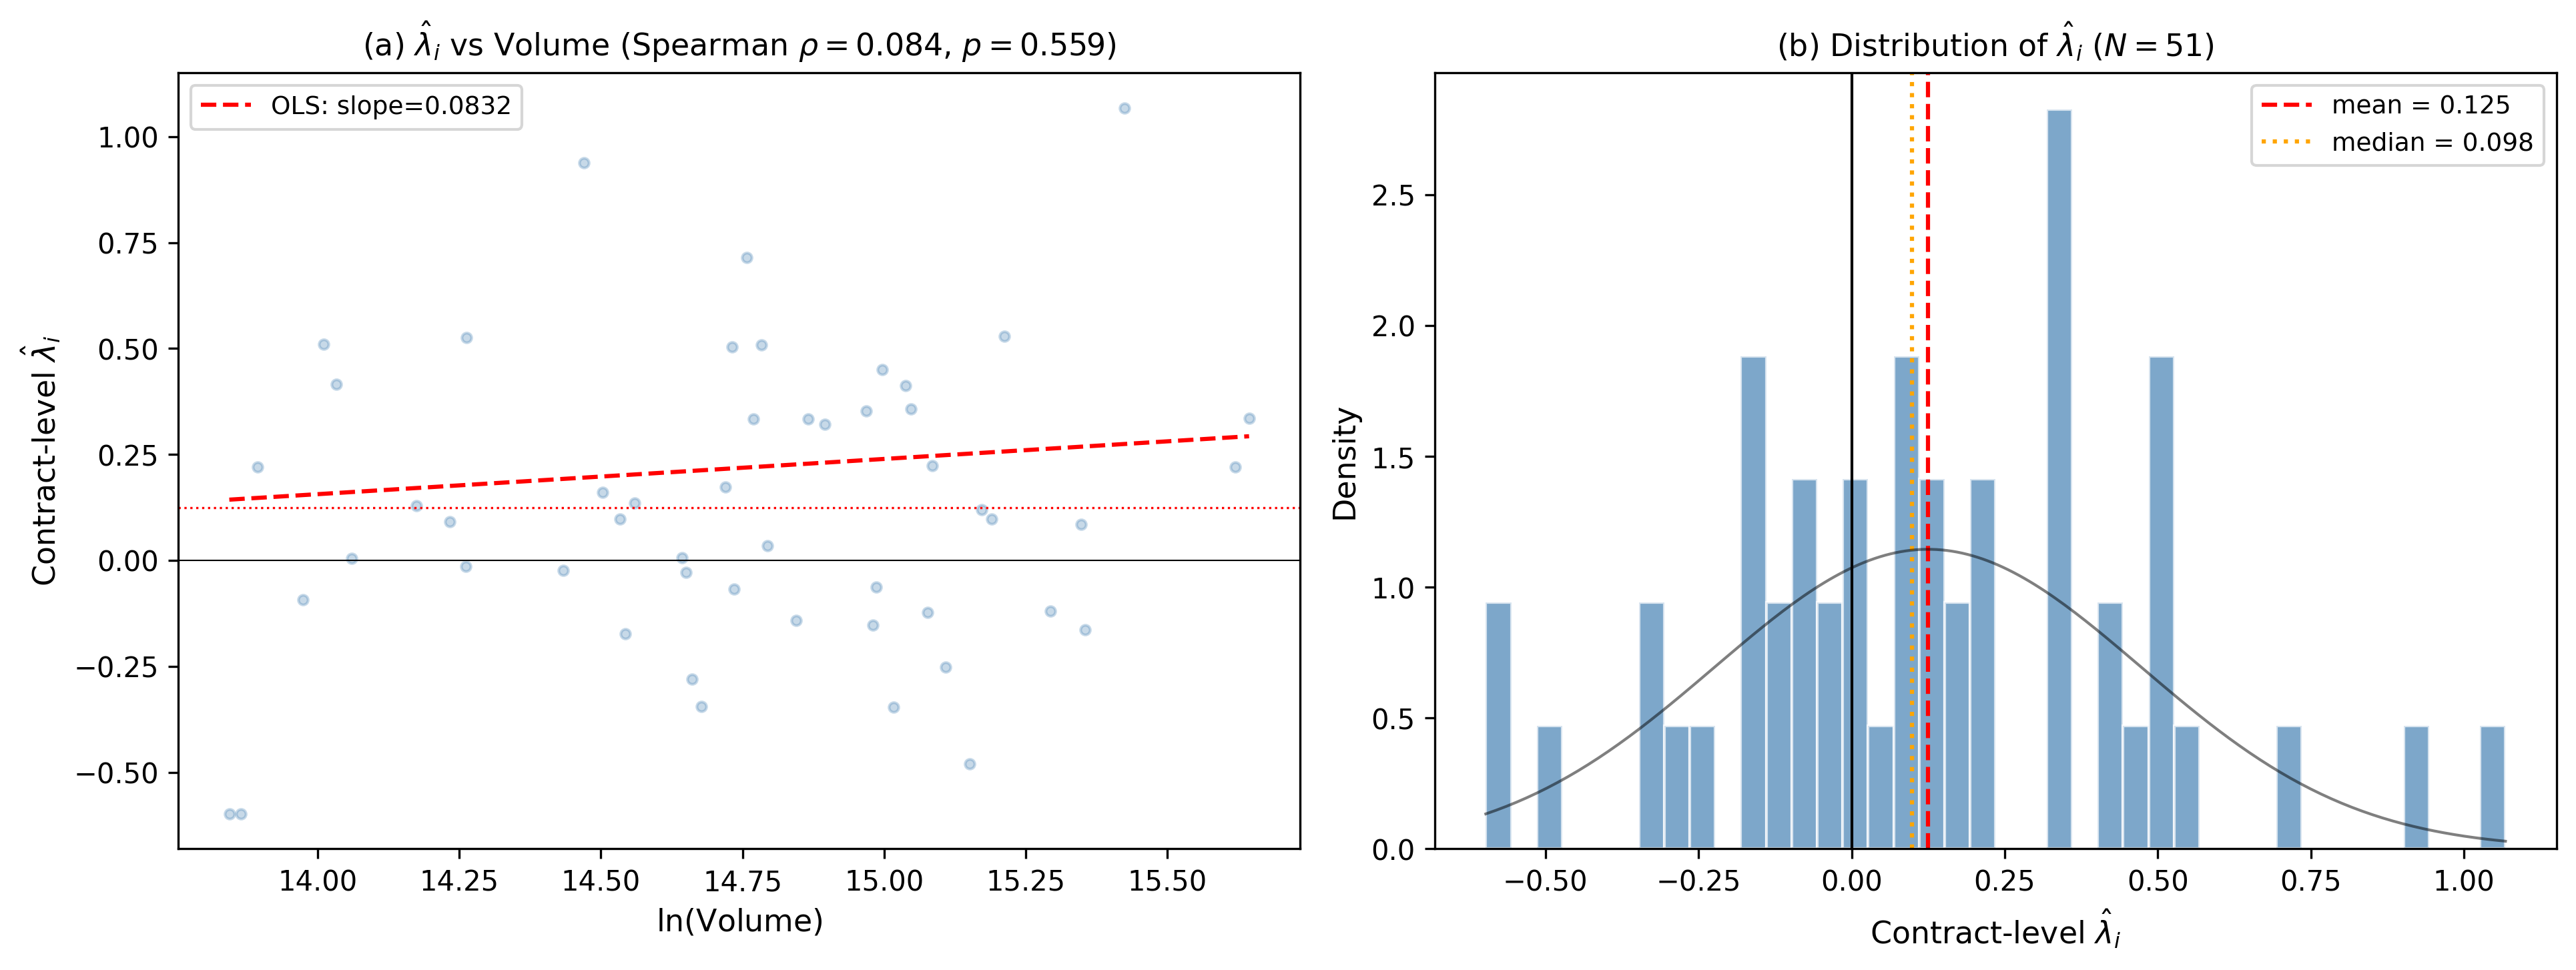
\includegraphics[width=0.95\textwidth]{fig_lambda_nba_external.png}
\caption{External benchmark: contract-level $\hat{\lambda}_i$ for 51 NBA game contracts. Panel (a): $\hat{\lambda}_i$ versus $\ln(\text{Volume})$; the Spearman correlation is small and insignificant. Panel (b): distribution of $\hat{\lambda}_i$, with mean $= 0.125$ and median $= 0.099$, both positive. The distribution is centered above zero, consistent with a positive pricing wedge.}
\label{fig:lambda_nba_external}
\end{figure}

\textbf{Asymmetric Wang extension.} The non-constant bin-level
\(\hat{\lambda}_k\) in Table\textasciitilde{}\ref{tab:calibration} and
the complement-invariant attenuation on the expanded sample both suggest
that the pricing wedge varies with probability level. To test this
directly, I estimate an asymmetric extension that allows the wedge to
depend linearly on the probability:
\[\lambda(p) = \lambda_0 + \lambda_1 \cdot (\tfrac{1}{2} - p)\] where
\(\lambda_0\) is the baseline wedge and \(\lambda_1\) captures the
asymmetry: \(\lambda_1 > 0\) implies longshots carry disproportionately
larger wedges than favorites. When \(\lambda_1 = 0\), the specification
reduces to the standard Wang transform. The market price under this
extension is
\(p^{\text{mkt}} = \Phi(\Phi^{-1}(p^*) + \lambda_0 + \lambda_1(1/2 - p^*))\),
estimated by maximum likelihood with numerical inversion.

\begin{table}[H]
\centering
\small
\caption{Asymmetric Wang extension: $\lambda(p) = \lambda_0 + \lambda_1(1/2 - p)$. The LR test compares the asymmetric model (2 parameters) against the standard Wang ($\lambda_1 = 0$, 1 parameter). Bootstrap confirmation on Kalshi (2,000 replications): $\hat{\lambda}_1 = 0.448 \pm 0.035$, 95\% CI excludes zero.}
\label{tab:asymmetric_wang}
\begin{tabular}{lrrrrrrr}
\toprule
Sample & $N$ & $\hat{\lambda}_0$ & $\hat{\lambda}_1$ & SE$(\lambda_1)$ & LR $\chi^2$ & $p$-value \\
\midrule
Polymarket 12-day & 2,460 & 0.145 & $+$0.287 & 0.169 & 2.5 & 0.112 \\
Polymarket 28-day & 13,824 & 0.183 & $-$0.191$^{*}$ & 0.089 & 5.0 & 0.025 \\
Kalshi & 200,253 & 0.076 & $+$0.448$^{***}$ & 0.014 & 808.0 & $<10^{-15}$ \\
\bottomrule
\end{tabular}
\end{table}

Allowing the pricing wedge to vary linearly with probability level
reveals a strong asymmetry on Kalshi (\(N = 200{,}253\)), where
longshots carry systematically larger wedges than favorites
(\(\hat{\lambda}_1 = 0.448\), \(p < 10^{-15}\)). Under the fitted model,
the implied fair-pricing threshold is \(p^* \approx 0.67\): contracts
above this probability are, on average, underpriced relative to their
physical probabilities. The asymmetric extension substantially closes
the gap between Wang and logistic specifications on Kalshi
(\(\Delta\text{AIC}\) from 818 to 12), indicating that standard Wang's
underperformance on left-skewed exchange data reflects the
constant-\(\lambda\) restriction rather than a failure of the
probit-based distortion family.

On Polymarket, the evidence is mixed: \(\hat{\lambda}_1\) is positive
but insignificant on the 12-day subsample (\(p = 0.112\)), and
marginally significant with opposite sign on the 28-day sample
(\(\hat{\lambda}_1 = -0.191\), \(p = 0.025\)). The negative estimate on
the expanded sample is consistent with sample-composition or
platform-ecology differences, including a greater share of
longer-duration and favorite-heavy contracts. For this reason, the
one-parameter Wang transform remains the paper's primary specification:
it is BIC-optimal in the one-parameter class, has axiomatic and
equilibrium foundations (Section\textasciitilde3.3), and provides
cross-platform comparability. The asymmetric extension is reported as a
robustness refinement for platform-specific distributional
heterogeneity, not as a replacement for the parsimonious baseline.

\begin{figure}[H]
\centering
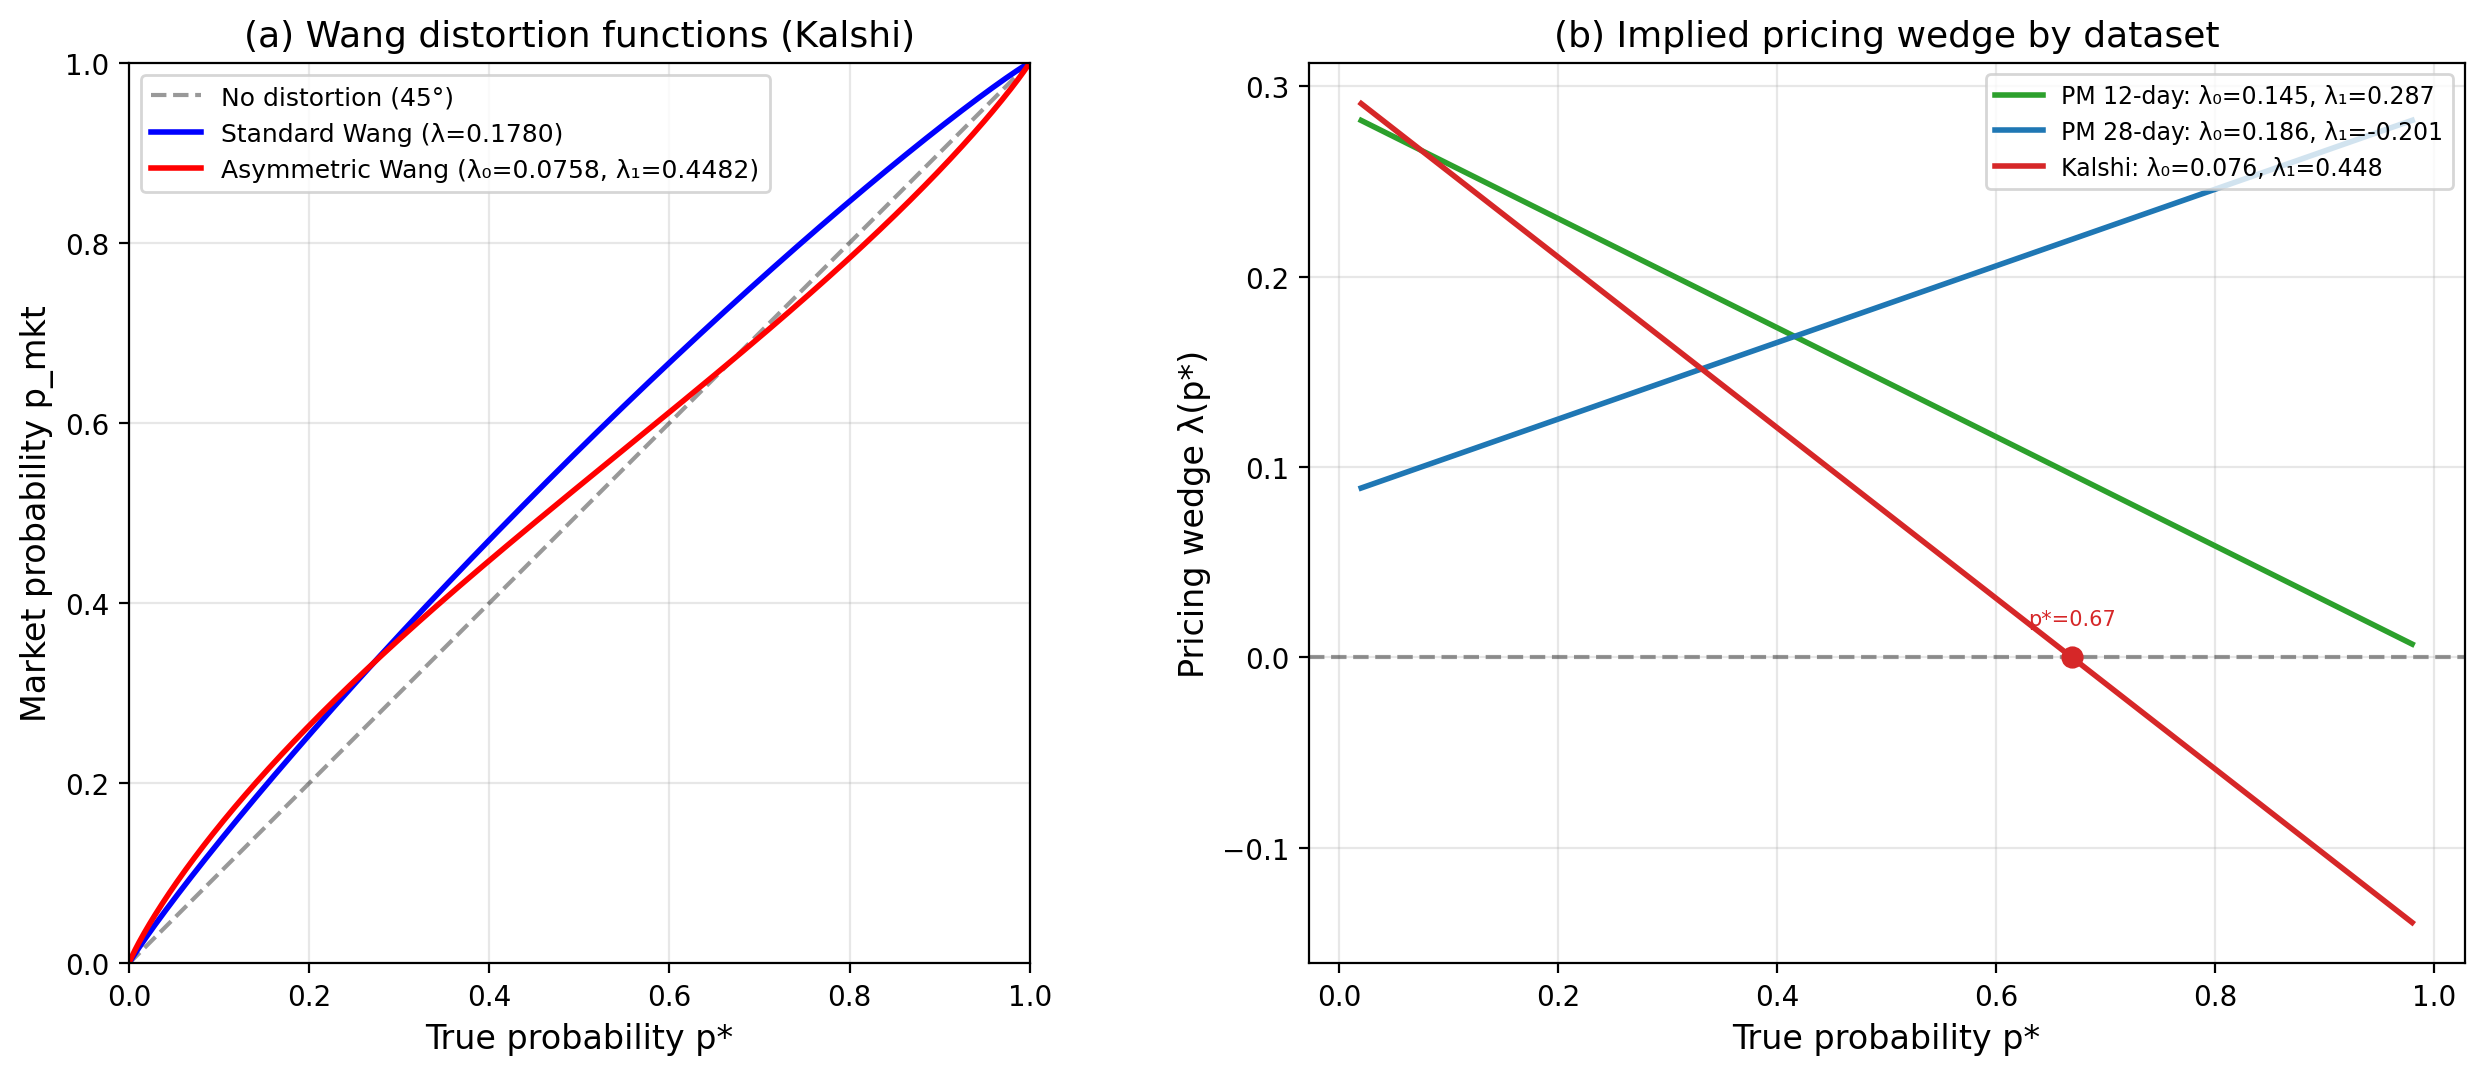
\includegraphics[width=0.95\textwidth]{fig_asymmetric_wang.png}
\caption{Asymmetric Wang distortion curves. The solid curves show the fitted distortion $p^{\text{mkt}} = \Phi(\Phi^{-1}(p^*) + \lambda_0 + \lambda_1(1/2 - p^*))$ for Polymarket (12-day and 28-day) and Kalshi. The dashed line is perfect calibration ($p^{\text{mkt}} = p^*$). On Kalshi, the strong positive $\hat{\lambda}_1$ generates a steeper distortion for longshots ($p^* < 0.5$) than for favorites, consistent with the asymmetric FLB pattern and the implied fair-pricing threshold at $p^* \approx 0.67$.}
\label{fig:asymmetric_wang}
\end{figure}

\begin{center}\rule{0.5\linewidth}{0.5pt}\end{center}

\section{Cross-Platform and Extended Sample
Validation}\label{cross-platform-and-extended-sample-validation}

The primary calibration in Section 5 uses Polymarket data from a single
platform over a limited time window. To establish that the positive Wang
parameter is a robust feature of prediction markets rather than a
platform- or period-specific artifact, I estimate
\(\hat{\lambda}_{MLE}\) across eight data sources spanning six
platforms, multiple years, and \(N = 291{,}309\) total contracts.

\subsection{Cross-Platform
Comparison}\label{cross-platform-comparison}

Table \ref{tab:cross_platform} reports Wang parameter estimates for each
data source. The estimation procedure is identical to Section 5.2:
Bernoulli MLE with standard errors from the numerical Hessian.

\begin{table}[H]
\centering
\small
\caption{Cross-platform Wang parameter estimates. All real-money platforms exhibit $\hat{\lambda} > 0$ (positive pricing wedge). Manifold, a play-money platform, shows $\hat{\lambda} < 0$ (overconfidence). Pooled estimate across all sources: $\hat{\lambda} = 0.183$ (SE $= 0.003$).}
\label{tab:cross_platform}
\begin{tabular}{lrrrrrr}
\toprule
Platform & $N$ & $\hat{\lambda}_{MLE}$ & SE & LR stat & $p$-value & Period \\
\midrule
Polymarket (CLOB) & 13,738 & 0.166$^{***}$ & 0.011 & 212.1 & $<10^{-15}$ & 2026 \\
Polymarket (2025) & 985 & 0.143$^{**}$ & 0.045 & 10.3 & 0.001 & 2025 \\
Polymarket (forecasting) & 579 & 0.013 & 0.056 & 0.1 & 0.813 & 2015--2024 \\
Kalshi & 271,699 & 0.187$^{***}$ & 0.003 & 3,186.0 & $<10^{-15}$ & 2021--2026 \\
Metaculus & 1,845 & 0.287$^{***}$ & 0.033 & 76.1 & $<10^{-15}$ & 2015--2024 \\
Good Judgment Open & 692 & 0.570$^{***}$ & 0.055 & 111.5 & $<10^{-15}$ & 2015--2024 \\
INFER & 90 & 0.635$^{***}$ & 0.180 & 13.7 & $<0.001$ & 2015--2024 \\
Manifold (play-money) & 1,681 & $-$0.218$^{***}$ & 0.032 & 45.8 & $<10^{-11}$ & 2015--2024 \\
\midrule
\textbf{Pooled (all)} & \textbf{291,309} & \textbf{0.183}$^{***}$ & \textbf{0.003} & \textbf{3,420.4} & $<10^{-15}$ & 2015--2026 \\
\bottomrule
\end{tabular}
\end{table}

\begin{figure}[H]
\centering
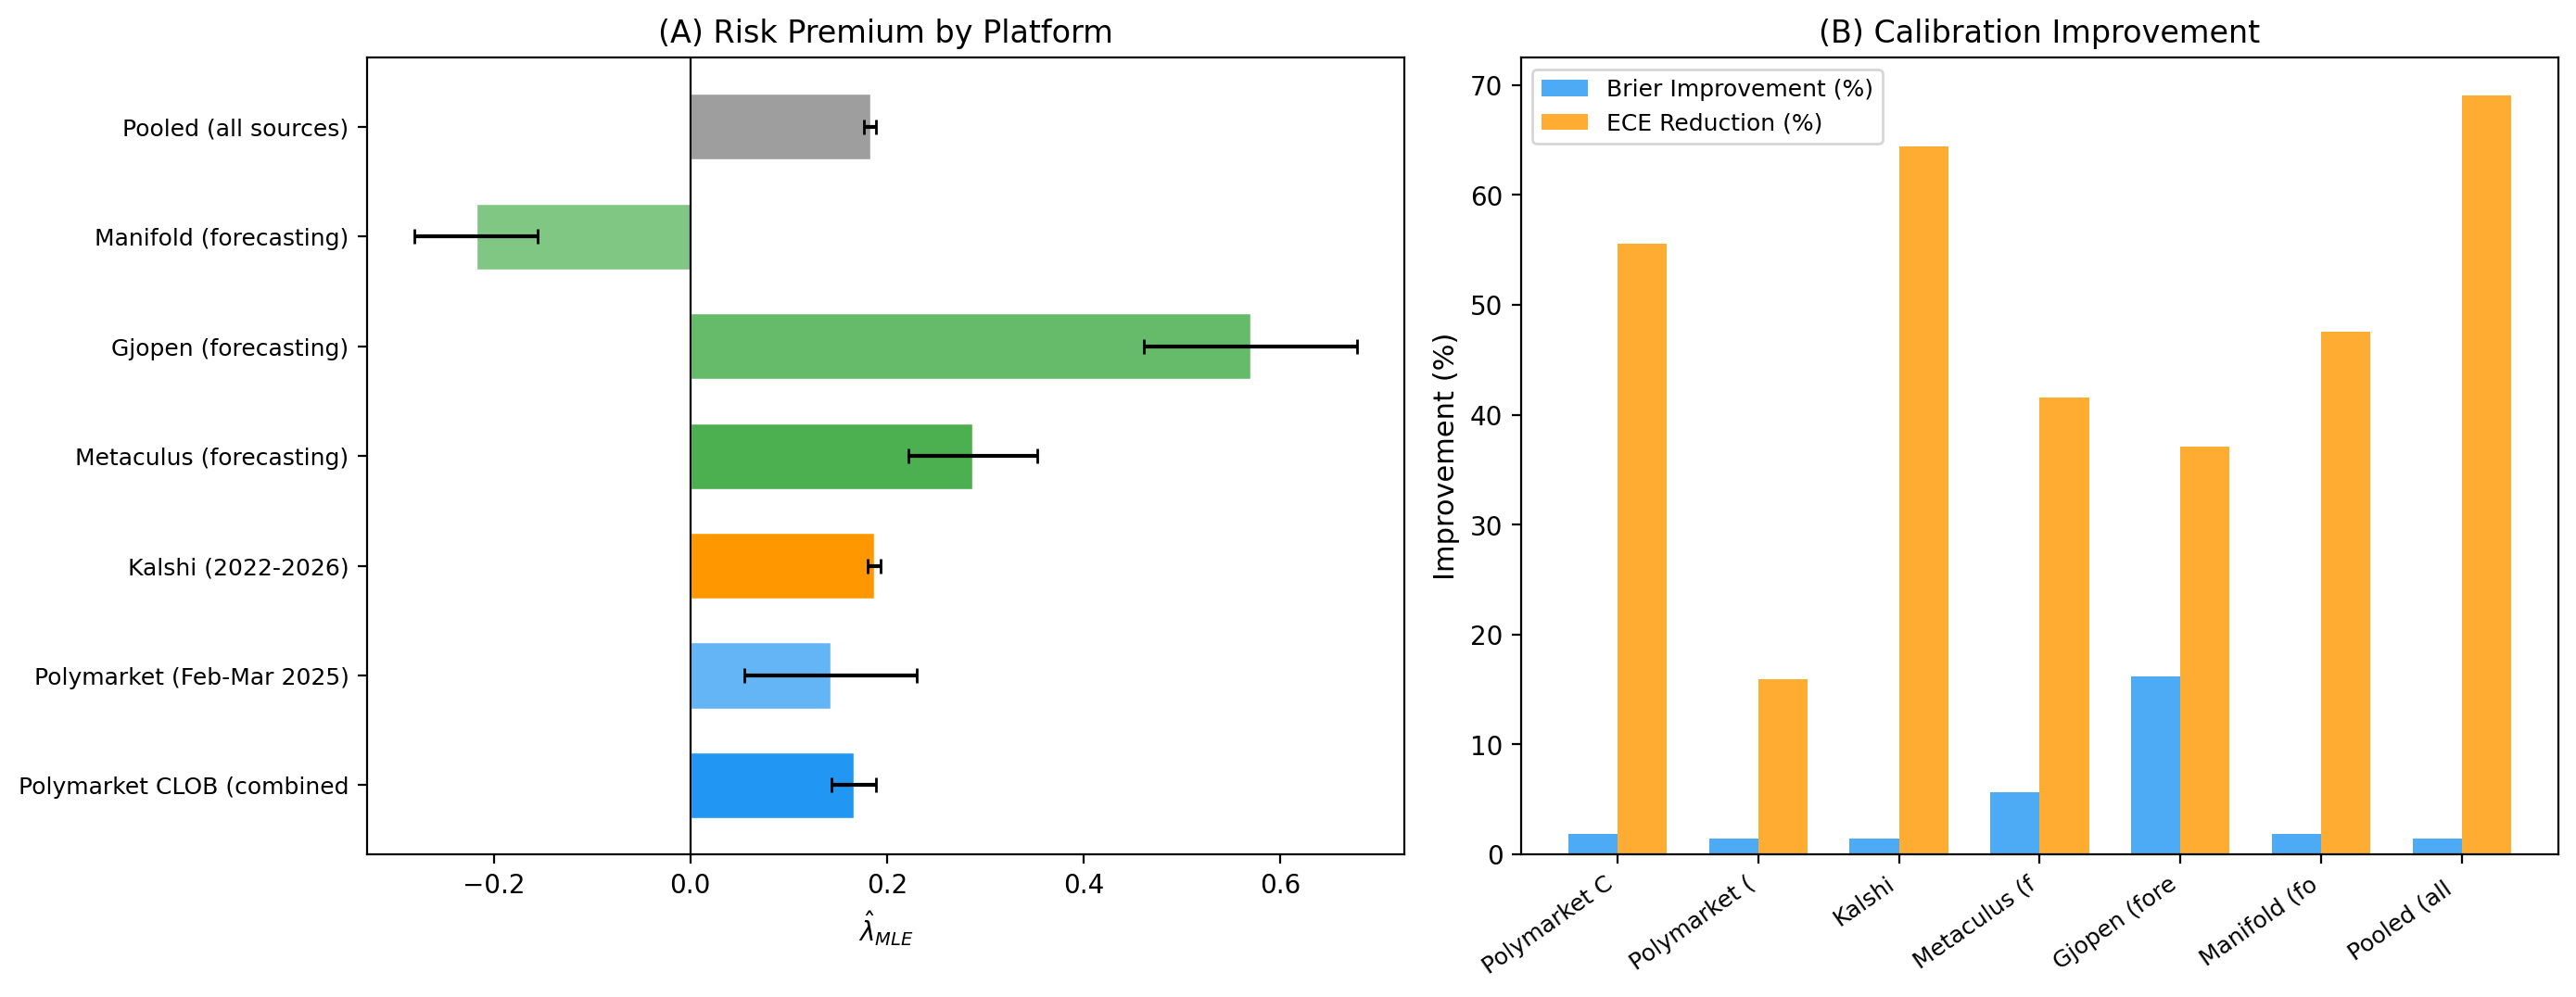
\includegraphics[width=\textwidth]{fig14_cross_platform.png}
\caption{Cross-platform Wang parameter estimates with 95\% confidence intervals. All real-money platforms exhibit $\hat{\lambda} > 0$; the play-money platform Manifold shows $\hat{\lambda} < 0$, consistent with overconfidence absent financial stakes. The pooled estimate (gray band) is $\hat{\lambda} = 0.183 \pm 0.006$.}
\end{figure}

\textbf{Key findings from the cross-platform analysis:}

\begin{enumerate}
\def\labelenumi{\arabic{enumi}.}
\item
  \textbf{Universality of the positive pricing wedge.} Every
  traded-contract platform---whether blockchain-based (Polymarket) or
  CFTC-regulated (Kalshi)---exhibits a statistically significant
  positive \(\hat{\lambda}\). The forecasting platforms (Metaculus, Good
  Judgment Open, INFER), which operate as prediction tournaments with
  reputational or prize-based incentives rather than direct financial
  risk, also show \(\hat{\lambda} > 0\), suggesting the distortion
  extends beyond traditional market settings---though the economic
  interpretation differs, as participants on these platforms do not bear
  financial risk in the same sense as on traded-contract venues.
\item
  \textbf{Magnitude gradient.} The pricing wedge increases with market
  friction and participant expertise: Polymarket
  (\(\hat{\lambda} \approx 0.15\)--\(0.17\)) \(<\) Kalshi
  (\(\hat{\lambda} = 0.19\)) \(<\) Metaculus (\(\hat{\lambda} = 0.29\))
  \(<\) Good Judgment Open (\(\hat{\lambda} = 0.57\)). This gradient is
  consistent with the liquidity effect documented in Section 5.3:
  platforms with deeper liquidity and more sophisticated participants
  exhibit smaller pricing wedges.
\item
  \textbf{Play-money control.} Manifold Markets, where participants
  trade with play-money tokens, exhibits a significant \textit{negative}
  \(\hat{\lambda} = -0.218\) (\(p < 10^{-11}\)). This is consistent with
  overconfidence: absent real financial stakes, participants overstate
  their confidence in event outcomes, pushing prices beyond physical
  probabilities in the opposite direction from the pricing wedge
  observed on real-money platforms. The play-money result provides a
  natural placebo test: it is inconsistent with purely behavioral
  explanations of \(\lambda > 0\) and supports the presence of a
  nontrivial risk-bearing component on real-money platforms.
\item
  \textbf{Consistency across Polymarket samples.} The 2025 Polymarket
  sample (\(\hat{\lambda} = 0.143\)) and the 2026 CLOB sample
  (\(\hat{\lambda} = 0.166\)) yield estimates within one standard error
  of each other, confirming temporal stability within the same platform.
\end{enumerate}

\textbf{Cross-platform covariate heterogeneity.} A one-stage
hierarchical MLE on the Kalshi sample (\(N = 200{,}226\)) yields
covariate signs reversed relative to the Polymarket opening-price
specification. A timing-ladder diagnostic---re-estimating the Polymarket
model at four lifecycle points (5\%, 20\%, 50\%, 80\%)---shows strict
monotonic convergence toward the Kalshi coefficient pattern: the \(L_1\)
distance between the Polymarket and Kalshi slope vectors falls from
1.033 at 5\% to 0.651 at 80\%, a 37\% reduction. However, no Polymarket
coefficient changes sign even at the latest timing point, implying that
price timing explains a substantial share, but not all, of the
cross-platform gap. Additional diagnostic evidence indicates that the
remaining difference is consistent with Kalshi's concentration in
short-duration contracts (86.9\% have duration \(< 24\) hours) and
broader differences in contract ecology and market microstructure. I
therefore interpret the cross-platform covariate differences as a
measurement- and composition-sensitive heterogeneity result, rather than
as evidence that either platform's risk-premium structure falsifies the
other. Details are reported in Appendix\textasciitilde A.

\subsection{Temporal Stability: Kalshi
Year-by-Year}\label{temporal-stability-kalshi-year-by-year}

The Kalshi dataset, with \(N = 200{,}253\) contracts (filtered to
\(p \in (0.05, 0.95)\)) spanning 2021--2026, permits a year-by-year
analysis of temporal stability. Table \ref{tab:kalshi_temporal} reports
annual estimates.

\begin{table}[H]
\centering
\small
\caption{Kalshi Wang parameter by year. The pricing wedge is consistently positive and significant across all years with sufficient sample size, with $\hat{\lambda} \in [0.14, 0.29]$.}
\label{tab:kalshi_temporal}
\begin{tabular}{lrrrrl}
\toprule
Year & $N$ & $\hat{\lambda}_{MLE}$ & SE & LR stat & Significance \\
\midrule
2021 & 199 & 0.047 & 0.106 & 0.2 & n.s. \\
2022 & 2,319 & 0.195$^{***}$ & 0.033 & 35.9 & $p < 10^{-8}$ \\
2023 & 6,118 & 0.144$^{***}$ & 0.020 & 54.4 & $p < 10^{-13}$ \\
2024 & 10,182 & 0.169$^{***}$ & 0.016 & 114.0 & $p < 10^{-15}$ \\
2025 & 12,362 & 0.290$^{***}$ & 0.015 & 393.3 & $p < 10^{-15}$ \\
2026 & 169,072 & 0.172$^{***}$ & 0.004 & 2,049.1 & $p < 10^{-15}$ \\
\bottomrule
\end{tabular}
\end{table}

\begin{figure}[H]
\centering
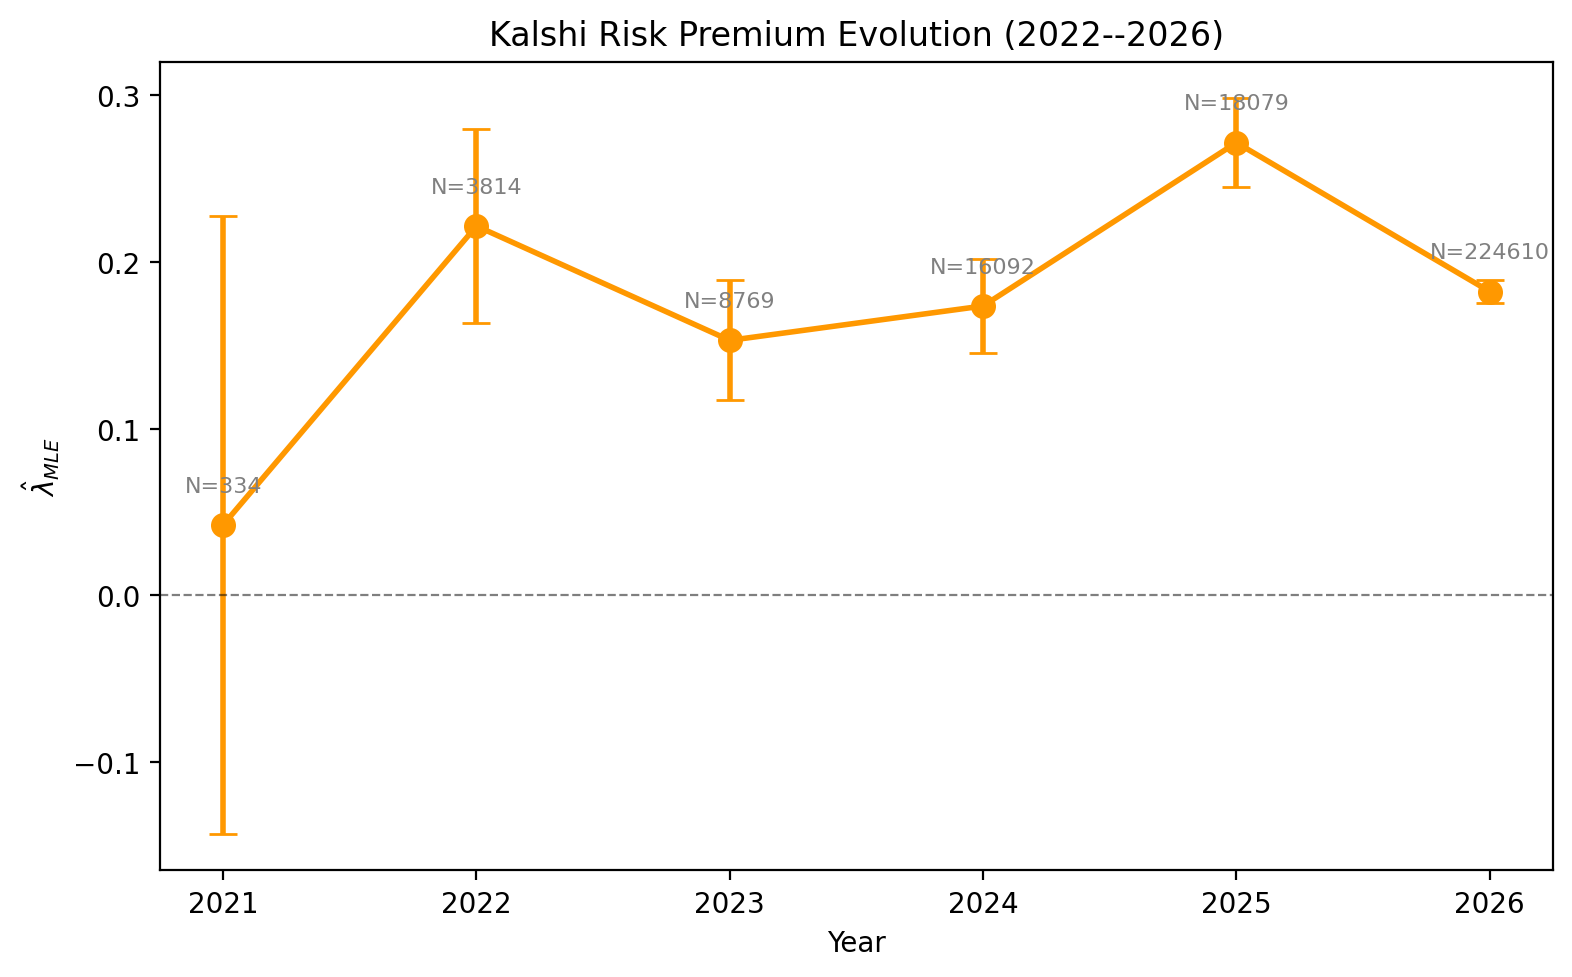
\includegraphics[width=\textwidth]{fig15_kalshi_temporal.png}
\caption{Kalshi Wang parameter estimates by year with 95\% CIs. The pricing wedge is consistently positive across 2022--2026, with year-to-year variation that may reflect changing market composition, regulatory environment, and participant base. The 2021 estimate is insignificant due to small sample size ($N = 199$).}
\end{figure}

The temporal analysis reveals several patterns: (i) the Wang parameter
is consistently positive and significant across all years with
sufficient data (\(N > 1{,}000\)); (ii) the range
\(\hat{\lambda} \in [0.14, 0.29]\) is remarkably stable given the rapid
growth of Kalshi's market over this period (from 199 settled contracts
in 2021 to 169,072 in 2026); (iii) the 2025 estimate
(\(\hat{\lambda} = 0.290\)) is the highest, potentially reflecting the
surge of retail participation during the 2024 U.S. presidential election
cycle and its aftermath.

\subsection{Discussion}\label{discussion}

The cross-platform results have three implications for the theoretical
framework:

First, the positive \(\lambda\) is not a microstructure artifact. It
persists across centralized limit order books (Polymarket, Kalshi) and
forecasting tournaments (Metaculus, GJ Open), which have fundamentally
different price formation mechanisms. This suggests that the pricing
wedge is intrinsic to prediction markets as an asset class, consistent
with the incomplete market interpretation in Section 3.

Second, the magnitude gradient across platforms is consistent with the
liquidity-premium hypothesis: deeper, more efficient markets price risk
more aggressively, shrinking the wedge between market prices and
physical probabilities. The convergence of Polymarket and Kalshi
estimates (\(\hat{\lambda}_P = 0.166\) vs.~\(\hat{\lambda}_K = 0.187\))
suggests that as both platforms mature and attract institutional flow,
the pricing wedge is being competed toward a common equilibrium level.

Third, the Manifold result (\(\hat{\lambda} < 0\)) provides a natural
placebo test for the pricing wedge mechanism. When the financial channel
is shut off (play-money), the pricing wedge vanishes and is replaced by
overconfidence. This is difficult to reconcile with purely behavioral
explanations of the FLB (e.g., probability weighting), which should
operate identically whether or not real money is at stake. The sign
reversal supports the presence of a nontrivial risk-bearing component in
\(\hat{\lambda}\) on real-money platforms, though the exact composition
of the pricing wedge---how much reflects risk-bearing costs versus other
market-structure forces---remains an open question.

\begin{center}\rule{0.5\linewidth}{0.5pt}\end{center}

\section{Extensions}\label{extensions}

\subsection{Event Implied
Volatility}\label{event-implied-volatility}

The log-odds framework yields a natural volatility measure, though care
is needed to distinguish two related but distinct objects.

\textbf{Model-implied EIV.} Under the baseline model (Section 3.2), a
latent information state \(S_t\) drives the physical probability via
\(p_t^* = \Phi(S_t / (\sigma\sqrt{\tau}))\), where
\(S_T \mid S_t \sim N(S_t, \sigma^2\tau)\) and the event occurs iff
\(S_T > 0\). Inverting gives
\(S_t = \sigma\sqrt{\tau} \cdot \Phi^{-1}(p_t)\). The
\emph{model-implied Event Implied Volatility} is:

\[\sigma_{\text{EIV}} = \frac{S_t}{\sqrt{\tau} \cdot \Phi^{-1}(p_t)} = \sigma\]

which recovers the model's belief volatility parameter \(\sigma\) by
construction. Note that \(S_t\) is a latent information state distinct
from the observed log-odds \(x_t = \text{logit}(p_t)\); the logit and
probit functions are approximately proportional
(\(\text{logit}(p) \approx (\pi/\sqrt{3}) \cdot \Phi^{-1}(p)\)), so the
qualitative properties carry over, but the ratio
\(x_t / \Phi^{-1}(p_t)\) is not constant and is undefined at
\(p = 0.5\).

\textbf{Empirical (realized) event volatility.} Separately, the realized
event volatility is the rolling annualized standard deviation of
log-odds increments:

\[\widehat{\sigma}_{\text{realized}}(t) = \text{sd}(\Delta x_{t-w}, \ldots, \Delta x_t) \times \sqrt{N_{\text{ann}}}\]

This is analogous to the implied-vs-realized volatility distinction in
equity options: the model-implied EIV is a theoretical construct derived
from the pricing formula, while the realized measure is computed
directly from observed price movements.

\begin{figure}[H]
\centering
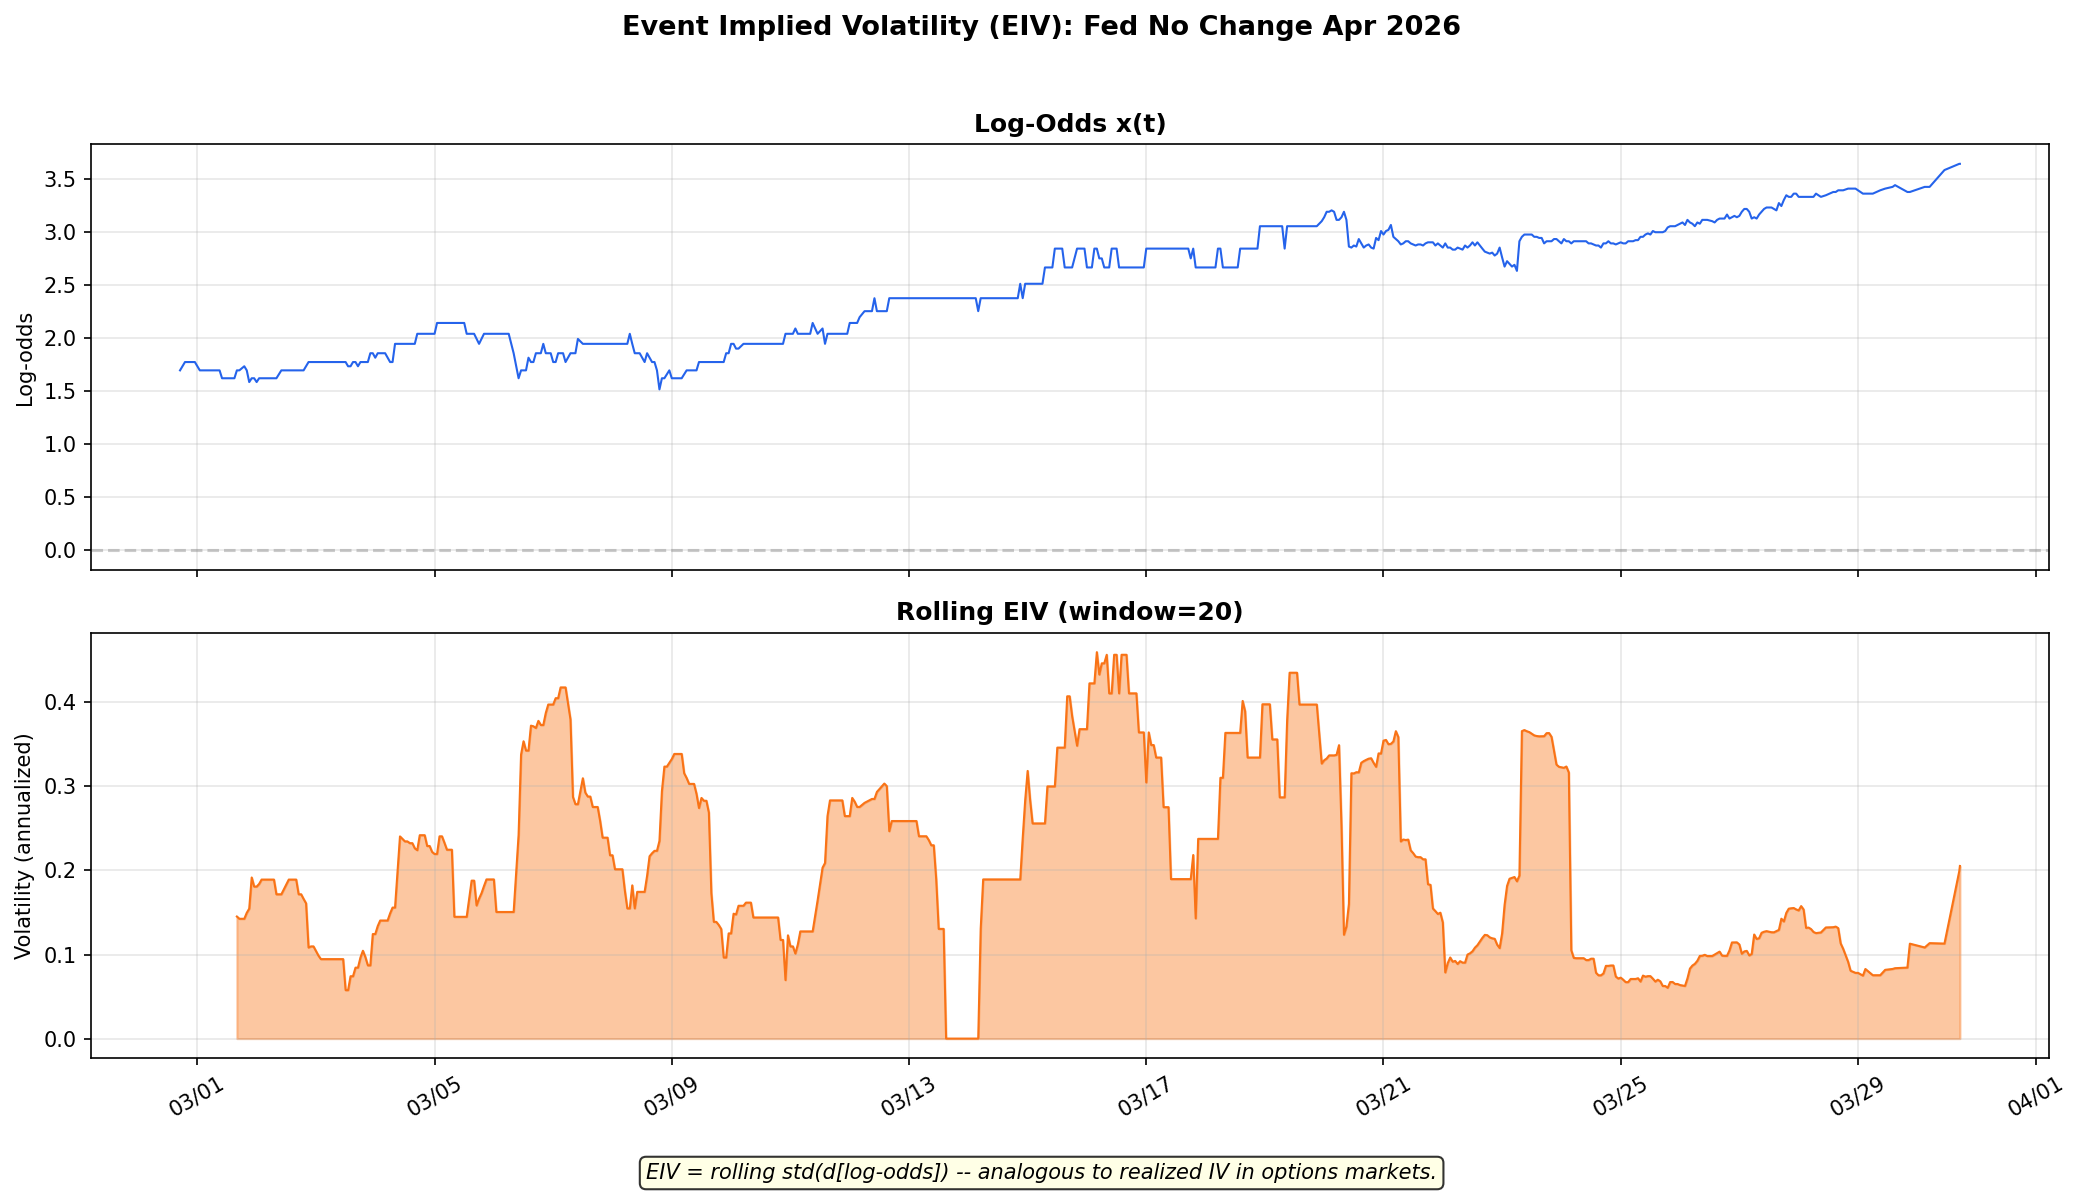
\includegraphics[width=\textwidth]{analysis_eiv_Fed_No_Change_Apr_2026.png}
\caption{Event Implied Volatility for the Fed ``No Change'' contract (Polymarket, hourly). EIV exhibits clear volatility clustering (ARCH effect), with periods of elevated uncertainty followed by mean-reversion.}
\end{figure}

\begin{figure}[H]
\centering
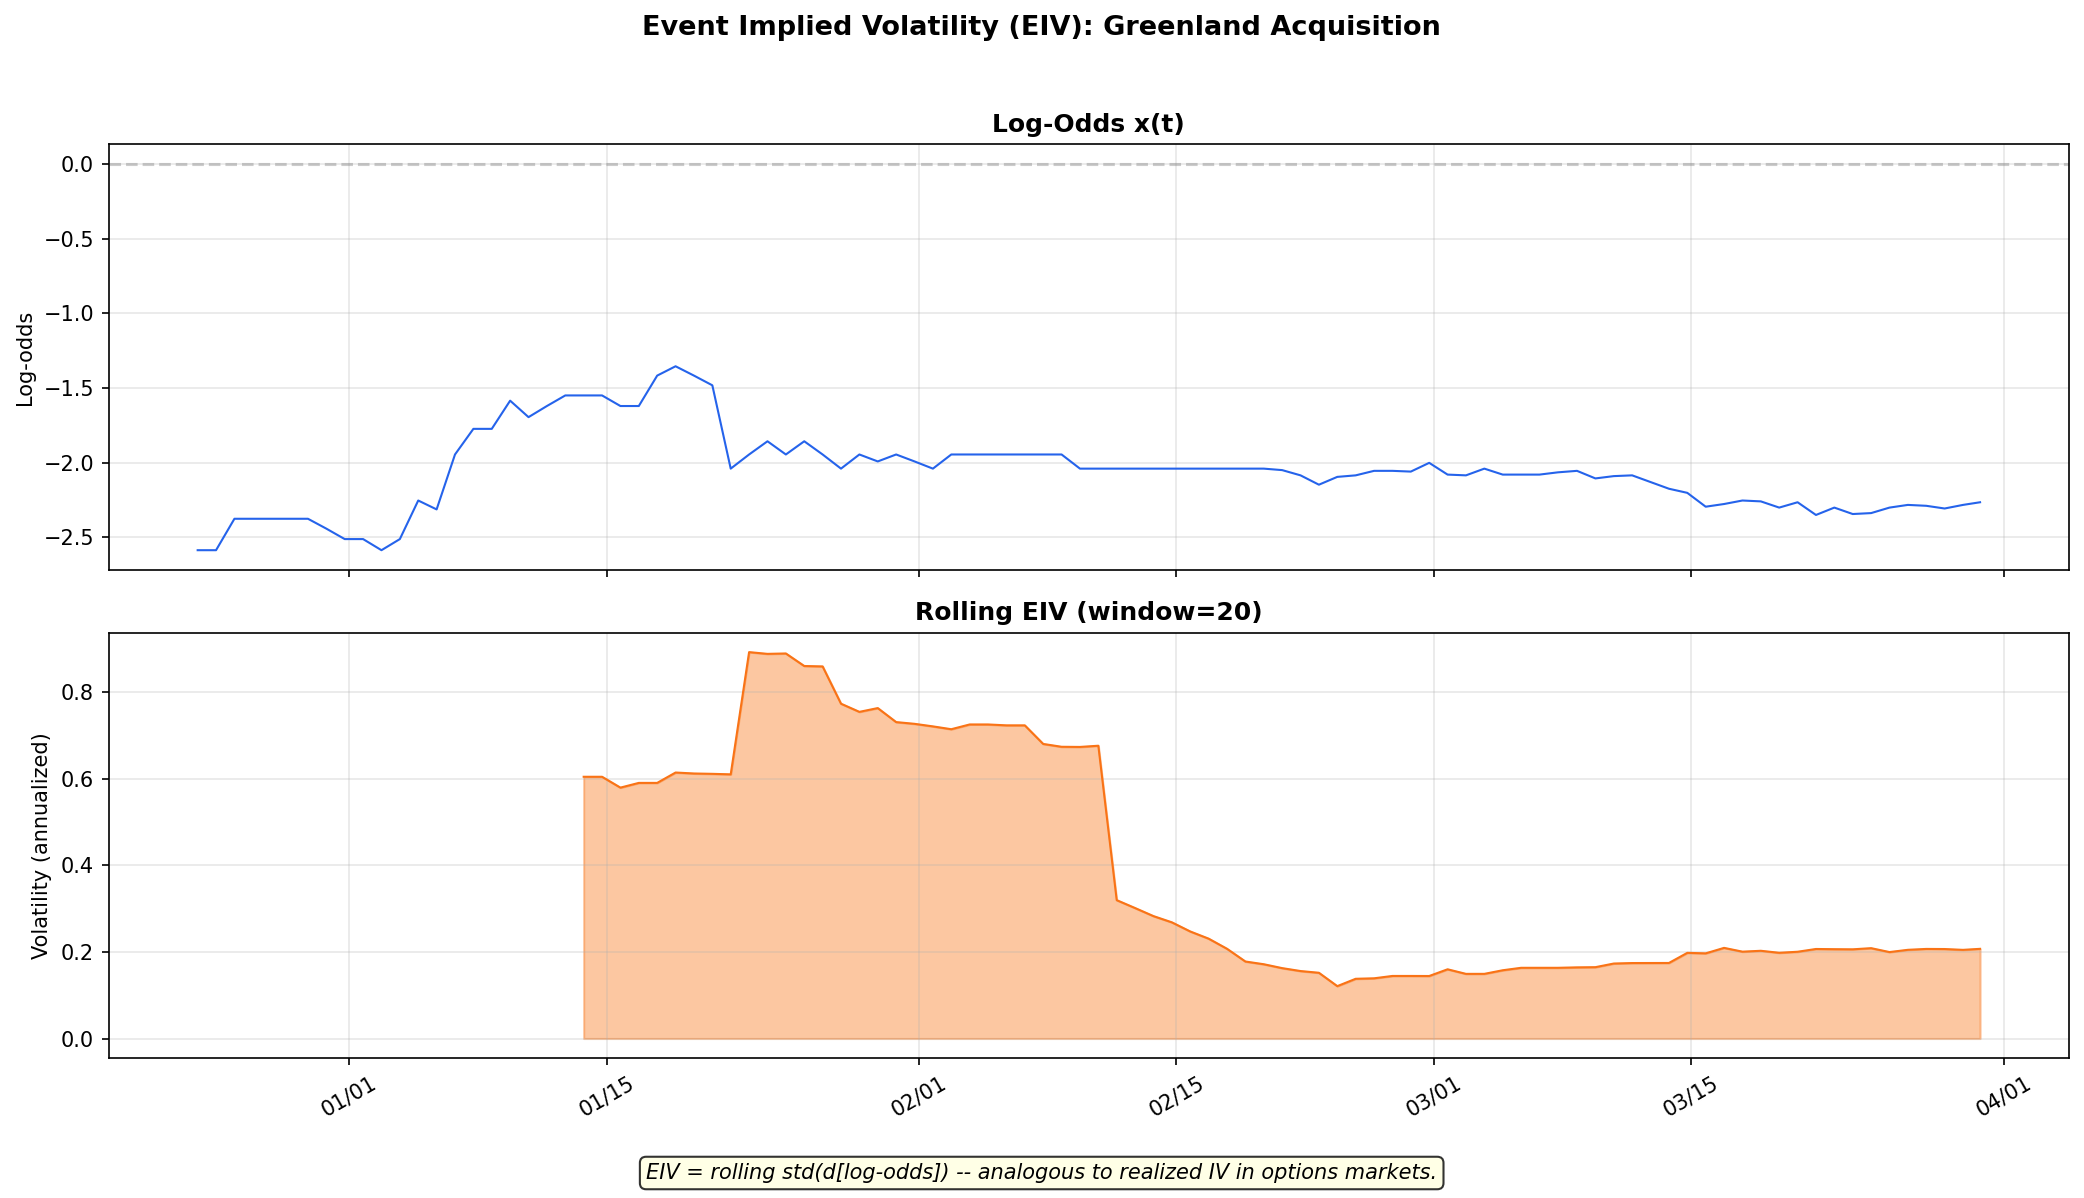
\includegraphics[width=\textwidth]{analysis_eiv_Greenland_Acquisition.png}
\caption{EIV for the Greenland acquisition contract (Polymarket, daily). The mid-January spike coincides with Trump administration statements; EIV decays as the market digests information, consistent with information arrival models (Easley and O'Hara, 1992).}
\end{figure}

EIV provides a descriptive tool for measuring the rate of probability
revision---conceptually related to realized volatility measures in
equity markets, though not directly analogous to the VIX, which is
derived from option-implied volatilities. Combined with the Wang
transform, it offers a two-dimensional characterization of prediction
market contracts: \(\lambda\) captures the level of the pricing wedge,
while \(\sigma_{\text{EIV}}\) captures the rate of information arrival.

\textbf{Cross-contract empirical distribution.} To move beyond case
studies, I compute realized event volatility for all \(N = 14{,}406\)
contracts with \(\geq 20\) hourly price observations, using a rolling
window of \(w = 10\) observations and annualizing by \(\sqrt{8{,}760}\).
Table \ref{tab:eiv_summary} reports the cross-sectional distribution.
The median annualized realized volatility is
\(\hat{\sigma}_{\text{realized}} = 5.31\), with substantial right skew
(mean \(= 12.54\)) and wide interquartile range \([1.52, 16.73]\).
Crypto contracts exhibit the highest median volatility (\(11.99\)),
followed by Tech (\(14.06\)) and Politics (\(8.64\)); Sports contracts
cluster near the overall median (\(5.50\)). Volume has negligible
correlation with realized volatility (Spearman \(\rho = 0.015\),
\(p = 0.10\)), suggesting that EIV captures information arrival
intensity rather than liquidity effects.

An ARCH(1) Lagrange multiplier test on squared log-odds increments
rejects the null of no volatility clustering at the 5\% level for 22.4\%
of contracts (\(3{,}231\) out of \(14{,}406\)), confirming that
volatility clustering---a hallmark of financial time series (Cont,
2001)---is present in a substantial fraction of prediction market
contracts. The rejection rate varies by category: Crypto contracts show
the highest clustering (35\%), consistent with the speculative dynamics
in digital asset markets, while Sports contracts show the lowest (12\%),
consistent with information arriving in discrete bursts (game outcomes)
rather than continuous flow.

\begin{table}[H]
\centering
\small
\caption{Cross-contract distribution of realized event volatility $\hat{\sigma}_{\text{realized}}$, computed as the median rolling standard deviation of hourly log-odds increments (annualized, window $= 10$). Contracts with $\geq 20$ hourly observations.}
\label{tab:eiv_summary}
\begin{tabular}{lrrrrr}
\toprule
Group & $N$ & Median & IQR & Mean & ARCH(1) rej.\ rate \\
\midrule
All contracts & 14,406 & 5.31 & [1.52, 16.73] & 12.54 & 22\% \\
\midrule
\textit{By category} & & & & & \\
\quad Sports & 3,731 & 5.50 & [1.92, 17.70] & 14.01 & 12\% \\
\quad Politics & 603 & 8.64 & [1.66, 15.84] & 13.99 & 20\% \\
\quad Crypto & 910 & 11.99 & [0.00, 20.70] & 14.56 & 35\% \\
\quad Tech & 654 & 14.06 & [0.59, 29.60] & 19.24 & 18\% \\
\quad Other & 8,508 & 4.39 & [1.36, 14.61] & 11.07 & 26\% \\
\midrule
\textit{By volume tier} & & & & & \\
\quad Low ($<$\$500) & 4,664 & 2.71 & [0.00, 11.47] & 10.37 & 23\% \\
\quad Med (\$500--2K) & 2,533 & 5.44 & [2.14, 17.57] & 14.47 & 19\% \\
\quad High (\$2K--10K) & 2,522 & 8.34 & [2.33, 19.62] & 14.81 & 21\% \\
\quad Very high ($>$\$10K) & 4,687 & 7.15 & [2.35, 18.13] & 12.45 & 24\% \\
\bottomrule
\end{tabular}
\end{table}


\begin{figure}[H]
\centering
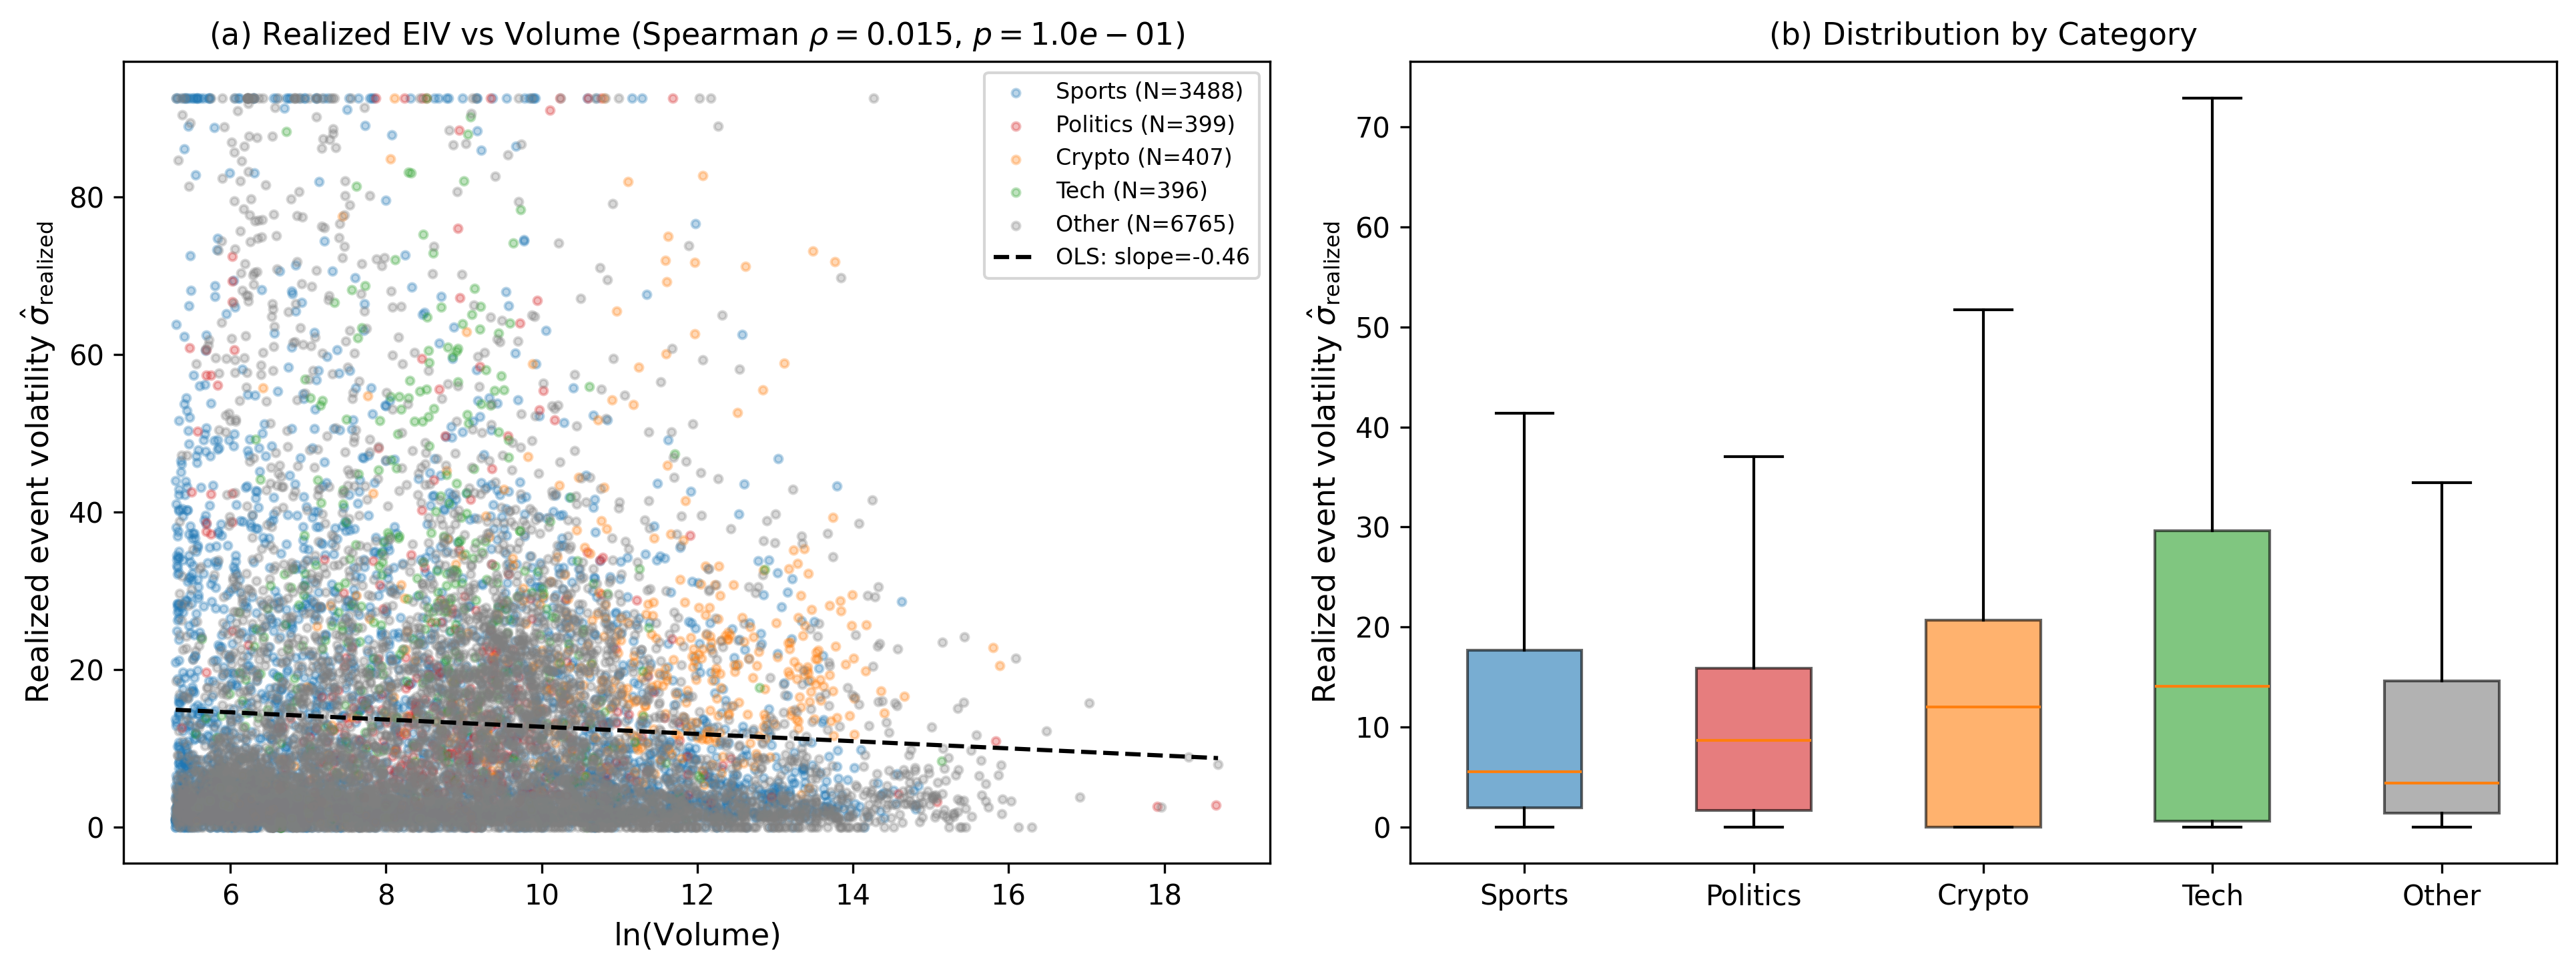
\includegraphics[width=\textwidth]{fig_eiv_distribution.png}
\caption{Cross-contract distribution of realized event volatility. Panel (a): scatter of $\hat{\sigma}_{\text{realized}}$ against $\ln(\text{Volume})$, colored by event category; the OLS line (slope $= -0.46$) and Spearman rank correlation ($\rho = 0.015$, $p = 0.10$) confirm negligible volume--volatility association. Panel (b): box plots by category, showing Crypto and Tech contracts exhibit higher and more dispersed realized volatility than Sports or Politics.}
\label{fig:eiv_distribution}
\end{figure}

\subsection{Hazard Rate Term
Structure}\label{hazard-rate-term-structure}

This section presents a theoretical extension that awaits empirical
implementation; current data limitations prevent successful calibration,
as discussed below.

For events with contracts at multiple maturities
\(T_1 < T_2 < \cdots < T_n\), the framework extends to an event hazard
rate term structure. Define the event intensity:

\[h(t) = -\frac{d}{dt}\ln(1 - p^*(t))\]

\textbf{Procedure:}

\begin{enumerate}
\def\labelenumi{\arabic{enumi}.}
\tightlist
\item
  \textbf{Strip pricing wedge}:
  \(\hat{p}_i^* = \Phi(\Phi^{-1}(p_i^{\text{mkt}}) - \hat{\lambda})\)
\item
  \textbf{Bootstrap hazard rates}:
  \(\hat{h}_i = -[\ln(1-\hat{p}_i^*) - \ln(1-\hat{p}_{i-1}^*)]\,/\,(T_i - T_{i-1})\)
\item
  \textbf{Parameterize} with Nelson-Siegel:
\end{enumerate}

\[h(T) = \beta_0 + \beta_1 \frac{1-e^{-T/\tau}}{T/\tau} + \beta_2\left(\frac{1-e^{-T/\tau}}{T/\tau} - e^{-T/\tau}\right)\]

This is directly analogous to CDS curve bootstrapping in credit markets:
strip the pricing wedge, extract default intensities, and fit a
parametric term structure. The analogy is suggestive: a prediction
market contract on ``event \(E\) occurs by time \(T\)'' is structurally
similar to a credit default swap on ``entity \(X\) defaults by time
\(T\),'' with \(h(t)\) playing the role of the default intensity. This
hazard rate extension does not appear to have been explored in the
prediction market literature.

\textbf{Empirical feasibility.} A systematic search of the current
sample identifies 16 multi-maturity contract families (same event,
\(\geq 3\) expiry dates). However, the bootstrapped hazard rates are
noisy: most families have closely spaced maturities (often created
simultaneously with different resolution dates), producing extreme or
negative point estimates of \(\hat{h}_i\). Nelson-Siegel fitting fails
to converge for all 16 families. The hazard rate term structure thus
remains a theoretical extension; empirical implementation at scale
requires multi-maturity contract data with well-separated expiry
dates---a data structure that may become available as prediction markets
mature and exchanges begin listing standardized maturity strips for
recurring events (e.g., monthly employment reports, quarterly GDP
releases).

\begin{center}\rule{0.5\linewidth}{0.5pt}\end{center}

\section{Conclusion}\label{conclusion}

This paper has proposed a pricing and decomposition framework for
prediction markets---an asset class that, despite annualized trading
volumes exceeding \$50 billion across major
platforms\footnote{Based on Polymarket monthly volumes of \$2--5 billion (source: Dune Analytics) and Kalshi's reported settlement volumes, annualized industry activity reaches this order of magnitude, though no single authoritative aggregate series exists.},
has lacked the theoretical infrastructure available to equities,
options, credit, and fixed income. The framework rests on three pillars:
a log-odds state variable, a diffusion-based dynamics specification, and
a Wang transform pricing wedge decomposition. The central observation,
rooted in Manski (2006) and formalized here, is that prediction markets
are \emph{incomplete}: no replication argument pins down a unique price,
so observed prices embed both event probability and a pricing wedge. The
Wang transform layer offers a single-parameter decomposition that
separates the two, and generates the favorite-longshot bias as a direct
mathematical consequence.

The empirical results support the framework across multiple dimensions.
Contract-level calibration on 2,460 Polymarket contracts yields a
statistically significant positive pricing wedge
(\(\hat{\lambda}_{MLE} = 0.176\), \(p < 10^{-10}\)), confirmed on an
expanded 28-day sample (\(N = 13{,}738\), \(\hat{\lambda} = 0.166\)).
Cross-platform validation on \(N = 291{,}309\) contracts across
Polymarket, Kalshi, Metaculus, Good Judgment Open, and INFER yields a
pooled estimate of \(\hat{\lambda} = 0.183\) (SE \(= 0.003\)), with
every real-money platform exhibiting a significant positive pricing
wedge. The play-money platform Manifold shows \(\hat{\lambda} = -0.22\),
providing a natural control that is inconsistent with purely behavioral
explanations and supports the presence of a nontrivial risk-bearing
component in \(\lambda > 0\) on real-money platforms. Year-by-year
Kalshi estimates over 2022--2026 confirm temporal stability
(\(\hat{\lambda} \in [0.14, 0.29]\)). The estimate is economically
interpretable: an event with 10\% physical probability trades at
approximately 13.5\%, a 35\% overpricing that longshot buyers
effectively pay as a pricing wedge. A one-stage hierarchical MLE jointly
estimates the baseline pricing wedge and covariate effects, confirming
that volume reduces the wedge (\(\hat{\beta}_{\text{vol}} < 0\)),
duration increases it (\(\hat{\beta}_{\text{dur}} > 0\)), and extremity
amplifies it (\(\hat{\beta}_{\text{ext}} < 0\); LR
\(\chi^2 = 361.3\))---generating the favorite-longshot bias pattern as a
direct consequence. A novel finding is that the pricing wedge is
time-varying: a stacked panel model with contract-clustered standard
errors reveals that the wedge is significant at market opening and
decays with a half-life of 33\% of contract lifetime (12-day sample),
with slower decay on the full 28-day sample where the minimum is reached
at 77\% of lifetime, linking the duration effect in the cross section to
the time-decay pattern within contracts. Four alternative opening-price
constructions yield \(\hat{\lambda} \in [0.131, 0.166]\), indicating
that approximately 80\% of the baseline estimate reflects the structural
pricing wedge rather than microstructure artifacts. An external
benchmark using Elo-model probabilities for 51 NBA contracts provides
independent directional support (\(\hat{\lambda} = 0.125\),
\(p = 0.014\)) without relying on ex-post resolution outcomes.

\textbf{Limitations.} The calibration approach is reduced-form;
separating the pricing wedge from behavioral probability distortion
(prospect theory weighting, overconfidence) requires instruments or
natural experiments. Candidates include regulatory shocks (Kalshi CFTC
ruling), the time-varying pattern documented in Section 5.4 (which
suggests market-microstructure rather than behavioral origins), and the
cross-platform dimension (same event, different \(\lambda\)). The
Manifold sign reversal (Section 6) provides suggestive evidence for the
risk-bearing interpretation but is not a definitive causal
identification. For the Kalshi cross-platform analysis, the available
price data is the last traded price before settlement rather than the
opening price used for Polymarket; this limits the interpretation of
calibration improvements (ECE, Brier score) for Kalshi, though the
\(\hat{\lambda}\) point estimates remain valid as they reflect the
systematic relationship between price levels and resolution rates. At
extreme probabilities, the elevated \(\hat{\lambda}\) may reflect
overconfidence rather than pure pricing wedge; the extended model finds
extremity is a significant predictor but cannot distinguish risk from
misperception. The external benchmark analysis (Section 5.6), using an
Elo rating model as an independent probability estimate for 51 NBA
contracts, provides directional support for a positive pricing wedge
(\(\hat{\lambda} = 0.125\), \(p = 0.014\)), though the sample is small
and the Elo model is noisier than sportsbook closing lines. Replication
with commercial closing-line data would strengthen this identification.

No prior work has applied the Wang transform to prediction markets, and
the empirical results---spanning 291,309 contracts across eight data
sources, six platforms, and eleven years---confirm that the framework
captures economically meaningful structure in the data. The framework
connects prediction market pricing to three established literatures: (i)
distortion risk measures in insurance mathematics (Wang, 2000; Yaari,
1987); (ii) the interpretation of prediction market prices in economics
(Manski, 2006; Wolfers and Zitzewitz, 2006); and (iii) incomplete market
pricing in mathematical finance (Harrison and Pliska, 1983). By bridging
these literatures, it provides practitioners with a principled,
model-dependent fair-value signal---subject to the reduced-form nature
of the calibration and the assumptions underlying the Wang
specification---and researchers with a testable structural model of
prediction market mispricing.

\vspace{1em}

\newpage

\section*{References}\label{references}

\begin{thebibliography}{99}
\small

\bibitem{ali1977} Ali, M.M. (1977). Probability and Utility Estimates for Racetrack
  Bettors. \emph{Journal of Political Economy}, 85(4), 803--815.

\bibitem{archak2009} Archak, N. and Ipeirotis, P.G. (2009). Modeling Volatility in
  Prediction Markets. \emph{Proceedings of the 10th ACM Conference on
  Electronic Commerce (EC '09)}.

\bibitem{artzner1999} Artzner, P., Delbaen, F., Eber, J.-M. and Heath, D. (1999). Coherent
  Measures of Risk. \emph{Mathematical Finance}, 9(3), 203--228.

\bibitem{avellaneda2008} Avellaneda, M. and Stoikov, S. (2008). High-Frequency Trading in a
  Limit Order Book. \emph{Quantitative Finance}, 8(3), 217--224.

\bibitem{barberis2008} Barberis, N. and Huang, M. (2008). Stocks as Lotteries: The
  Implications of Probability Weighting for Security Prices.
  \emph{American Economic Review}, 98(5), 2066--2100.

\bibitem{black1973} Black, F. and Scholes, M. (1973). The Pricing of Options and Corporate
  Liabilities. \emph{Journal of Political Economy}, 81(3), 637--654.

\bibitem{bürgi2025} Bürgi, C., Deng, W. and Whelan, K. (2025). Makers and Takers: The
  Economics of the Kalshi Prediction Market. \emph{CEPR Discussion
  Paper} 20631.

\bibitem{bühlmann1980} Bühlmann, H. (1980). An Economic Premium Principle. \emph{ASTIN
  Bulletin}, 11(1), 52--60.

\bibitem{cochrane2000} Cochrane, J.H. and Saa-Requejo, J. (2000). Beyond Arbitrage: Good-Deal
  Asset Price Bounds in Incomplete Markets. \emph{Journal of Political
  Economy}, 108(1), 79--119.

\bibitem{cont2001} Cont, R. (2001). Empirical Properties of Asset Returns: Stylized Facts
  and Statistical Issues. \emph{Quantitative Finance}, 1(2), 223--236.

\bibitem{dalen2025} Dalen, S. (2025). Toward Black Scholes for Prediction Markets: A
  Unified Kernel and Market Maker's Handbook. \emph{arXiv preprint},
  arXiv:2510.15205.

\bibitem{denneberg1994} Denneberg, D. (1994). \emph{Non-Additive Measure and Integral}. Kluwer
  Academic Publishers.

\bibitem{easley1992} Easley, D. and O'Hara, M. (1992). Time and the Process of Security
  Price Adjustment. \emph{Journal of Finance}, 47(2), 577--605.

\bibitem{frittelli2000} Frittelli, M. (2000). The Minimal Entropy Martingale Measure and the
  Valuation Problem in Incomplete Markets. \emph{Mathematical Finance},
  10(1), 39--52.

\bibitem{gilboa1989} Gilboa, I. and Schmeidler, D. (1989). Maxmin Expected Utility with
  Non-Unique Prior. \emph{Journal of Mathematical Economics}, 18(2),
  141--153.

\bibitem{gjerstad2004} Gjerstad, S. (2004). Risk Aversion, Beliefs, and Prediction Market
  Equilibrium. \emph{Working Paper}, University of Arizona.

\bibitem{gneiting2007} Gneiting, T., Balabdaoui, F. and Raftery, A.E. (2007). Probabilistic
  Forecasts, Calibration and Sharpness. \emph{Journal of the Royal
  Statistical Society: Series B}, 69(2), 243--268.

\bibitem{griffith1949} Griffith, R.M. (1949). Odds Adjustments by American Horse-Race
  Bettors. \emph{American Journal of Psychology}, 62(2), 290--294.

\bibitem{hamada2003} Hamada, M. and Sherris, M. (2003). Contingent Claim Pricing Using
  Probability Distortion Operators: Methods from Insurance Risk Pricing
  and Their Relationship to Financial Theory. \emph{Applied Mathematical
  Finance}, 10(1), 19--47.

\bibitem{hanson2007} Hanson, R. (2007). Logarithmic Market Scoring Rules for Modular
  Combinatorial Information Aggregation. \emph{Journal of Prediction
  Markets}, 1(1), 3--15.

\bibitem{harrison1981} Harrison, J.M. and Pliska, S.R. (1981). Martingales and Stochastic
  Integrals in the Theory of Continuous Trading. \emph{Stochastic
  Processes and their Applications}, 11(3), 215--260.

\bibitem{harrison1983} Harrison, J.M. and Pliska, S.R. (1983). A Stochastic Calculus Model of
  Continuous Trading: Complete Markets. \emph{Stochastic Processes and
  their Applications}, 15(3), 313--316.

\bibitem{hasbrouck1995} Hasbrouck, J. (1995). One Security, Many Markets: Determining the
  Contributions to Price Discovery. \emph{Journal of Finance}, 50(4),
  1175--1199.

\bibitem{he2013} He, Z. and Krishnamurthy, A. (2013). Intermediary Asset Pricing.
  \emph{American Economic Review}, 103(2), 732--770.

\bibitem{he2017} He, X.-Z. and Treich, N. (2017). Prediction Market Prices under Risk
  Aversion and Heterogeneous Beliefs. \emph{Journal of Mathematical
  Economics}, 70, 105--114.

\bibitem{hosmer2000} Hosmer, D.W. and Lemeshow, S. (2000). \emph{Applied Logistic
  Regression}, 2nd ed.~Wiley.

\bibitem{johnston2007} Johnston, M. (2007). Extension of the Capital Asset Pricing Model to
  Non-normal Dependence Structures. \emph{ASTIN Bulletin}, 37(1),
  35--52.

\bibitem{jullien2000} Jullien, B. and Salanié, B. (2000). Estimating Preferences under Risk:
  The Case of Racetrack Bettors. \emph{Journal of Political Economy},
  108(3), 503--530.

\bibitem{kass1995} Kass, R.E. and Raftery, A.E. (1995). Bayes Factors. \emph{Journal of
  the American Statistical Association}, 90(430), 773--795.

\bibitem{huang2024} Huang, H.H., Sun, J. and Zhang, S. (2024). Asset Pricing for the
  Lottery-Like Security Under Probability Weighting: Based on
  Generalized Wang Transform. \emph{North American Journal of Economics
  and Finance}, 71, 102078.

\bibitem{kijima2008} Kijima, M. and Muromachi, Y. (2008). An Extension of the Wang
  Transform Derived from Bühlmann's Economic Premium Principle for
  Insurance Risk. \emph{Insurance: Mathematics and Economics}, 42(3),
  887--896.

\bibitem{le2026} Le, N.A. (2026). Decomposing Crowd Wisdom: Domain-Specific Calibration
  Dynamics in Prediction Markets. \emph{arXiv preprint},
  arXiv:2602.19520.

\bibitem{liang1986} Liang, K.-Y. and Zeger, S.L. (1986). Longitudinal Data Analysis Using
  Generalized Linear Models. \emph{Biometrika}, 73(1), 13--22.

\bibitem{madrigal-cianci2026} Madrigal-Cianci, J.P., Monsalve Maya, C. and Breakey, L. (2026).
  Prediction Markets as Bayesian Inverse Problems: Uncertainty
  Quantification, Identifiability, and Information Gain from
  Price-Volume Histories under Latent Types. \emph{arXiv preprint},
  arXiv:2601.18815.

\bibitem{manski2006} Manski, C.F. (2006). Interpreting the Predictions of Prediction
  Markets. \emph{Economics Letters}, 91(3), 425--429.

\bibitem{mccullagh1989} McCullagh, P. and Nelder, J.A. (1989). \emph{Generalized Linear
  Models}, 2nd ed.~Chapman and Hall.

\bibitem{muravyev2013} Muravyev, D., Pearson, N.D. and Broussard, J.P. (2013). Is There Price
  Discovery in Equity Options? \emph{Journal of Financial Economics},
  107(2), 259--283.

\bibitem{ng2026} Ng, H., Peng, L., Tao, Y. and Zhou, D. (2026). Price Discovery and
  Trading in Modern Prediction Markets. \emph{SSRN Working Paper},
  5331995.

\bibitem{ostrovsky2012} Ostrovsky, M. (2012). Information Aggregation in Dynamic Markets with
  Strategic Traders. \emph{Econometrica}, 80(6), 2595--2647.

\bibitem{ottaviani2010} Ottaviani, M. and Sorensen, P.N. (2010). Noise, Information, and the
  Favorite-Longshot Bias in Parimutuel Predictions. \emph{American
  Economic Journal: Microeconomics}, 2(1), 58--85.

\bibitem{page2013} Page, L. and Clemen, R.T. (2013). Do Prediction Markets Produce
  Well-Calibrated Probability Forecasts? \emph{Economic Journal},
  123(568), 491--513.

\bibitem{pelsser2008} Pelsser, A. (2008). On the Applicability of the Wang Transform for
  Pricing Financial Risks. \emph{ASTIN Bulletin}, 38(1), 171--181.

\bibitem{rubinstein1991} Rubinstein, M. and Reiner, E. (1991). Unscrambling the Binary Code.
  \emph{Risk Magazine}, 4(9), 75--83.

\bibitem{servan-schreiber2004} Servan-Schreiber, E., Wolfers, J., Pennock, D.M. and Galebach, B.
  (2004). Prediction Markets: Does Money Matter? \emph{Electronic
  Markets}, 14(3), 243--251.

\bibitem{schmeidler1986} Schmeidler, D. (1986). Integral Representation without Additivity.
  \emph{Proceedings of the American Mathematical Society}, 97(2),
  255--261.

\bibitem{shin1991} Shin, H.S. (1991). Optimal Betting Odds Against Insider Traders.
  \emph{Economic Journal}, 101(408), 1179--1185.

\bibitem{shin1993} Shin, H.S. (1993). Measuring the Incidence of Insider Trading in a
  Market for State-Contingent Claims. \emph{Economic Journal}, 103(420),
  1141--1153.

\bibitem{snowberg2010} Snowberg, E. and Wolfers, J. (2010). Explaining the Favorite-Longshot
  Bias: Is It Risk-Love or Misperceptions? \emph{Journal of Political
  Economy}, 118(4), 723--746.

\bibitem{vuong1989} Vuong, Q.H. (1989). Likelihood Ratio Tests for Model Selection and
  Non-Nested Hypotheses. \emph{Econometrica}, 57(2), 307--333.

\bibitem{wang1996} Wang, S.S. (1996). Premium Calculation by Transforming the Layer
  Premium Density. \emph{ASTIN Bulletin}, 26(1), 71--92.

\bibitem{wang2000} Wang, S.S. (2000). A Class of Distortion Operators for Pricing
  Financial and Insurance Risks. \emph{Journal of Risk and Insurance},
  67(1), 15--36.

\bibitem{wang2003} Wang, S.S. (2003). Equilibrium Pricing Transforms: New Results Using
  Bühlmann's 1980 Economic Model. \emph{ASTIN Bulletin}, 33(1), 57--73.

\bibitem{wang2004} Wang, S.S. (2004). Cat Bond Pricing Using Probability Transforms.
  \emph{Geneva Papers: Études et Dossiers}, No.~278, 19--29.

\bibitem{wang1997} Wang, S.S., Young, V.R. and Panjer, H.H. (1997). Axiomatic
  Characterization of Insurance Prices. \emph{Insurance: Mathematics and
  Economics}, 21(2), 173--183.

\bibitem{whelan2024} Whelan, K. (2024). Risk Aversion and Favourite-Longshot Bias in a
  Competitive Fixed-Odds Betting Market. \emph{Economica}, 91(361),
  188--209.

\bibitem{wirch1999} Wirch, J.L. and Hardy, M.R. (1999). A Synthesis of Risk Measures for
  Capital Adequacy. \emph{Insurance: Mathematics and Economics}, 25(3),
  337--347.

\bibitem{wolfers2004} Wolfers, J. and Zitzewitz, E. (2004). Prediction Markets.
  \emph{Journal of Economic Perspectives}, 18(2), 107--126.

\bibitem{wolfers2006} Wolfers, J. and Zitzewitz, E. (2006). Interpreting Prediction Market
  Prices as Probabilities. \emph{NBER Working Paper} 12200.

\bibitem{yaari1987} Yaari, M.E. (1987). The Dual Theory of Choice Under Risk.
  \emph{Econometrica}, 55(1), 95--115.

\end{thebibliography}

\newpage

\appendix\section{Supplementary Tables}\label{appendix}

\begin{table}[H]
\centering
\small
\caption{Per-horizon separate MLEs (baseline calibration, 12-day subsample). These estimates are superseded by the stacked panel model (Section 5.4), which borrows strength across horizons and provides correct contract-clustered inference.}
\label{tab:horizons_appendix}
\begin{tabular}{lrrrrl}
\toprule
Lifetime \% & $N$ & $\hat{\lambda}_{MLE}$ & SE & 95\% CI & $p$-value \\
\midrule
5\% (Opening) & 2,460 & 0.176$^{***}$ & 0.027 & [0.123, 0.230] & $7.1 \times 10^{-11}$ \\
10\% & 2,409 & 0.158$^{***}$ & 0.027 & [0.104, 0.212] & $8.3 \times 10^{-9}$ \\
20\% & 2,316 & 0.110$^{***}$ & 0.028 & [0.055, 0.165] & $8.8 \times 10^{-5}$ \\
30\% & 2,236 & 0.082$^{**}$ & 0.029 & [0.026, 0.139] & 0.004 \\
40\% & 2,065 & 0.080$^{**}$ & 0.030 & [0.021, 0.138] & 0.008 \\
50\% (Mid-life) & 1,976 & 0.050 & 0.030 & [$-$0.010, 0.110] & 0.102 \\
60\% & 1,902 & 0.052 & 0.031 & [$-$0.008, 0.113] & 0.091 \\
70\% & 1,763 & 0.040 & 0.032 & [$-$0.023, 0.103] & 0.216 \\
80\% & 1,662 & 0.031 & 0.033 & [$-$0.035, 0.096] & 0.357 \\
90\% & 1,359 & 0.062 & 0.038 & [$-$0.011, 0.136] & 0.098 \\
\bottomrule
\end{tabular}
\end{table}

\begin{table}[H]
\centering
\small
\caption{One-stage hierarchical Wang MLE on Kalshi contracts. Dependent variable: binary outcome $y_i$. Model: $\Pr(y_i = 1) = \Phi(\Phi^{-1}(p_i^{\text{mkt}}) - X_i\beta)$. Fisher standard errors reported; sandwich robust SEs in brackets. Significance: $^{***}p<0.001$, $^{**}p<0.01$, $^{*}p<0.05$.}
\label{tab:kalshi_hierarchical}
\begin{tabular}{lrrrr}
\toprule
 & \multicolumn{2}{c}{Main spec} & \multicolumn{2}{c}{Year FE} \\
\cmidrule(lr){2-3} \cmidrule(lr){4-5}
Variable & Coef. & SE & Coef. & SE \\
\midrule
Constant & 0.1400$^{***}$ & (0.0198) & 0.3357$^{**}$ & (0.1102) \\
 & [0.0188] & & [0.1032] & \\
$\ln(\text{Volume})$ & 0.0384$^{***}$ & (0.0031) & 0.0300$^{***}$ & (0.0032) \\
 & [0.0029] & & [0.0031] & \\
$\ln(\text{Duration})$ & -0.1101$^{***}$ & (0.0032) & -0.1241$^{***}$ & (0.0035) \\
 & [0.0030] & & [0.0033] & \\
$|p - 0.5|$ & 0.1917$^{***}$ & (0.0267) & 0.1768$^{***}$ & (0.0268) \\
 & [0.0261] & & [0.0262] & \\
Year=2022 & & & 0.0725 & (0.1115) \\
 & & & [0.1045] & \\
Year=2023 & & & 0.0444 & (0.1083) \\
 & & & [0.1012] & \\
Year=2024 & & & 0.0028 & (0.1077) \\
 & & & [0.1005] & \\
Year=2025 & & & -0.0847 & (0.1079) \\
 & & & [0.1007] & \\
Year=2026 & & & -0.1272 & (0.1070) \\
 & & & [0.1001] & \\
\midrule
$N$ & \multicolumn{2}{r}{200,226} & \multicolumn{2}{r}{200,226} \\
Log-lik. & \multicolumn{2}{r}{-75541.5} & \multicolumn{2}{r}{-75475.4} \\
LR $\chi^2$ (covariates) & \multicolumn{2}{r}{1267.2} & \multicolumn{2}{r}{1399.4} \\
Pseudo $R^2$ & \multicolumn{2}{r}{0.024828} & \multicolumn{2}{r}{0.025681} \\
\bottomrule
\end{tabular}
\end{table}

\begin{table}[H]
\centering
\small
\caption{Cross-platform category-level Wang parameter comparison. Each cell reports $\hat{\lambda}_{MLE}$ estimated separately by category. $\Delta\lambda = \hat{\lambda}_{\text{Kalshi}} - \hat{\lambda}_{\text{Polymarket}}$; positive values indicate higher risk loading on the less liquid platform.}
\label{tab:cross_platform_category}
\begin{tabular}{lrrrrrrr}
\toprule
 & \multicolumn{3}{c}{Polymarket} & \multicolumn{3}{c}{Kalshi} & \\
\cmidrule(lr){2-4} \cmidrule(lr){5-7}
Category & $N$ & $\hat{\lambda}$ & SE & $N$ & $\hat{\lambda}$ & SE & $\Delta\lambda$ \\
\midrule
Sports & 973 & 0.070 & 0.042 & 122 & 0.573$^{***}$ & 0.158 & +0.503 \\
Politics & 71 & 0.054 & 0.157 & 750 & 0.400$^{***}$ & 0.066 & +0.346 \\
Crypto & 305 & 0.253 & 0.077 & 12,975 & 0.297$^{***}$ & 0.015 & +0.044 \\
Tech & 414 & 0.268 & 0.079 & 8,246 & -0.022 & 0.017 & -0.290 \\
Other & 692 & 0.282 & 0.051 & 178,133 & 0.178$^{***}$ & 0.004 & -0.104 \\
\midrule
\textit{Pooled} & 2,460 & 0.176 & 0.027 & 200,226 & 0.178$^{***}$ & 0.004 & +0.002 \\
\bottomrule
\end{tabular}
\end{table}

\begin{table}[H]
\centering
\small
\caption{Polymarket timing ladder: one-stage hierarchical Wang MLE estimated at different lifecycle pricing points. The Kalshi pooled estimate (using near-settlement prices) is shown in the last row for comparison. Robust (sandwich) standard errors in parentheses. Significance: $^{***}p<0.001$, $^{**}p<0.01$, $^{*}p<0.05$.}
\label{tab:polymarket_timing_ladder}
\resizebox{\textwidth}{!}{%
\begin{tabular}{lrcccc}
\toprule
Timing point & $N$ & $\hat{\beta}_0$ & $\hat{\beta}_{\text{vol}}$ & $\hat{\beta}_{\text{dur}}$ & $\hat{\beta}_{\text{ext}}$ \\
\midrule
PM 5\% (opening) & 13,274 & 0.2599$^{***}$ (0.0636) & -0.0716$^{***}$ (0.0053) & 0.1431$^{***}$ (0.0122) & -0.4778$^{***}$ (0.0985) \\
%% VERIFY: confirm PM 20%, 50%, 80% rows against estimation code before SSRN update
PM 20\% & 12,923 & 0.2097$^{**}$ (0.0646) & -0.0616$^{***}$ (0.0053) & 0.1248$^{***}$ (0.0125) & -0.3617$^{***}$ (0.0971) \\
PM 50\% (mid-life) & 12,645 & 0.1797$^{**}$ (0.0648) & -0.0541$^{***}$ (0.0053) & 0.1050$^{***}$ (0.0125) & -0.1907$^{*}$ (0.0956) \\
PM 80\% (late-life) & 10,697 & 0.2884$^{***}$ (0.0743) & -0.0467$^{***}$ (0.0056) & 0.0561$^{***}$ (0.0148) & -0.2079$^{*}$ (0.1026) \\
\midrule
Kalshi (near-settle.) & 200,226 & 0.1400$^{***}$ (0.0188) & 0.0384$^{***}$ (0.0029) & -0.1101$^{***}$ (0.0030) & 0.1917$^{***}$ (0.0261) \\
\midrule
\multicolumn{6}{l}{\textit{Sign comparison (Polymarket opening $\to$ Kalshi):}} \\
 &  & + $\to$ + \checkmark & $-$ $\to$ + $\times$ & + $\to$ $-$ $\times$ & $-$ $\to$ + $\times$ \\
\bottomrule
\end{tabular}%
}
\end{table}

\begin{table}[H]
\centering
\small
\caption{Distance between Polymarket and Kalshi slope coefficients at each timing point. $\Delta\beta_j = \hat{\beta}^{\text{PM}}_j - \hat{\beta}^{\text{Kalshi}}_j$ for each covariate $j$. Decreasing distances indicate convergence toward the Kalshi coefficient pattern.}
\label{tab:polymarket_vs_kalshi_distance}
\begin{tabular}{lcccccc}
\toprule
 & \multicolumn{3}{c}{Signed difference $\Delta\beta$} & \multicolumn{2}{c}{Distance} & \\
\cmidrule(lr){2-4} \cmidrule(lr){5-6}
Timing & $\Delta\beta_{\text{vol}}$ & $\Delta\beta_{\text{dur}}$ & $\Delta\beta_{\text{ext}}$ & $L_1$ & $L_2$ & Reduction \\
\midrule
PM 5\% (opening) & -0.1101 & +0.2532 & -0.6695 & 1.0328 & 0.7242 & --- \\
PM 20\% & -0.1000 & +0.2349 & -0.5535 & 0.8883 & 0.6095 & 14\% \\
PM 50\% (mid-life) & -0.0925 & +0.2151 & -0.3824 & 0.6900 & 0.4484 & 33\% \\
PM 80\% (late-life) & -0.0851 & +0.1662 & -0.3997 & 0.6510 & 0.4411 & 37\% \\
\bottomrule
\end{tabular}
\end{table}

\subsection{External Benchmark
Details}\label{b.-external-benchmark-details}

This appendix provides methodological details for the external benchmark
validation reported in Section 5.6.

\textbf{Elo model specification.} I build Elo ratings from the complete
2025--26 NBA regular season (1,135 games, 30 teams) using a standard
recursive update. The parameters are \(K = 28\) (update factor) and
home-court advantage \(= 42\) Elo points, calibrated to the modern NBA
home-win rate of approximately 56\%. All teams are initialized at Elo
\(= 1500\); preseason and All-Star games are excluded.

\textbf{Elo calibration.} The model achieves a Brier score of 0.218 on
the 1,135-game sample. Binned calibration shows reasonable alignment
between predicted and realized home-win rates, with the strongest
calibration in the 30--80\% predicted probability range.

\textbf{Sportsbook validation.} To validate the Elo model against a
sharper external benchmark, I compare its predictions to consensus
moneyline odds from The Odds API for 13 contemporaneous NBA games. The
consensus probability is the mean across nine bookmakers, with overround
removed by normalization. The correlation between Elo and sportsbook
probabilities is \(r = 0.618\), with MAE \(= 0.166\) and RMSE
\(= 0.200\). The moderate correlation confirms that the Elo model
captures a substantial share of the variation in sharp-market pricing,
while the residual noise inflates the contract-level \(\hat{\lambda}_i\)
estimates relative to what a sportsbook-based benchmark would yield.

\textbf{Matching procedure.} I identify Polymarket NBA game contracts by
regex matching on the title format ``Team A vs.~Team B'\,', requiring
both team names to normalize to one of 30 canonical NBA team names via
an alias table. Each contract is matched to the closest Elo game
involving the same team pair within a \([-1, +5]\)-day window around the
contract's creation date. Of 80 contracts passing team normalization, 51
are successfully matched; the 29 unmatched contracts reference games
outside the matching window or future unplayed games.

\textbf{Contract-level \(\hat{\lambda}_i\).} For each matched contract,
the Wang parameter is computed as
\(\hat{\lambda}_i = \Phi^{-1}(p_i^{\text{Polymarket}}) - \Phi^{-1}(\hat{p}_i^{\text{Elo}})\),
where \(p_i^{\text{Polymarket}}\) is the opening price (first-5\%
midpoint) and \(\hat{p}_i^{\text{Elo}}\) is the pre-game Elo probability
assigned to the first-named team.

\textbf{OLS regression.} A cross-sectional regression of
\(\hat{\lambda}_i\) on \(\ln(\text{Volume})\) and price extremity
\(|p_i - 0.5|\) finds neither covariate significant at conventional
levels (\(N = 51\); Table \ref{tab:external_benchmark}, Panel B), though
the negative extremity coefficient (\(\hat{\beta} = -0.72\),
\(p = 0.094\)) is suggestive of pricing wedge concentrated near
even-odds contracts. The limited power reflects the small matched
sample.

\end{document}
